\documentclass[a4paper,11pt,final]{report}

\usepackage[francais]{babel}
\usepackage[utf8]{inputenc}
\usepackage[T1]{fontenc}
\usepackage[pdftex]{graphicx}
\usepackage{setspace}
\usepackage{color}
\usepackage{makeidx}
\usepackage{blkarray}
\usepackage{verbatim}
\usepackage[final]{pdfpages} 
\usepackage{hyperref}
\usepackage{moreverb}
\usepackage{fancyvrb}
\usepackage{fancyhdr} %pour header
\usepackage[Lenny]{fncychap}
\usepackage[french]{varioref}
\usepackage [paper=a4paper,tmargin=2cm,bmargin=2.5cm,lmargin=3cm,rmargin=3cm]{geometry}
\usepackage{caption}
\usepackage{amsmath}% http://ctan.org/pkg/amsmath
\pagestyle{fancy}
\fancyhf{}
\renewcommand{\headrulewidth}{1pt} %barre header et foot
\renewcommand{\footrulewidth}{1pt}

\makeindex
\newcommand{\reporttitle}{\Huge{Interface Cerveau - Ordinateur à partir d'EEG}}    % Titre
\newcommand{\reportauthor}{
	\Large{Romain \textsc{Richard}}\\
	\Large{Florian \textsc{Lepont}}
	}% Auteur
\newcommand{\reportsubject}{\huge{GIN 956 : Rapport de Projet de Recherche et Développement }} % Sujet
\newcommand{\HRule}{\rule{\linewidth}{1.5mm}}

\setlength{\parskip}{1ex} % Espace entre les paragraphes

%entete et pied de page
\chead{Interface Cerveau - Ordinateur à partir d'EEG}
\lfoot{Faculté de Génie, UdeS}
\rfoot{\thepage}

\begin{document}
  \renewcommand{\contentsname}{Sommaire}  %change table des matiere en sommaire
  \begin{center}

\begin{minipage}[t]{1.1\textwidth}
  \begin{flushright}
    
\includegraphics [width=80mm,height=25mm]{images/logo_udes.png} \\[0.5cm]
  \end{flushright}
\end{minipage} \\[6cm]

\textsc{\Large \reportsubject}\\[1cm]
\HRule \\[0.25cm]
\textsc{\Large \reporttitle}
{
\HRule \\[4cm]
\begin{figure}[h]
	%\centering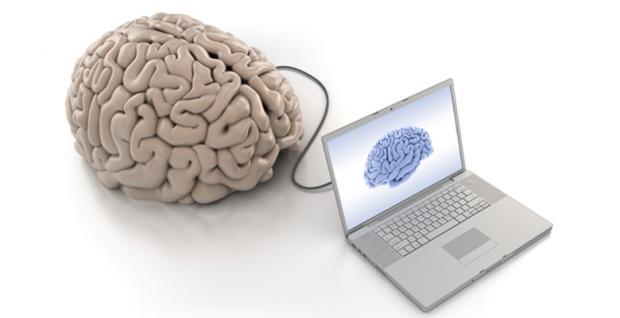
\includegraphics[width=14cm,height=7cm]{images/mainImage.jpg}
\end{figure}
\bigbreak\bigbreak\bigbreak\bigbreak
\begin{minipage}[t]{0.3\textwidth}
  \begin{flushleft} \large
    \emph{\Large{Étudiants :}}\\ 
    \reportauthor
  \end{flushleft}
\end{minipage}
\begin{minipage}[ht]{0.6\textwidth}
  \begin{flushright} \large
    \emph{\Large{Professeur responsable :}} \\
    \Large{M.~Jean \textsc{Rouat}}
  \end{flushright}
\end{minipage}
}
\vfill

{\large Hiver 2015}

\thispagestyle{empty} %pas afficher num page

\end{center}


  %\newpage\null\newpage
  \chapter*{Remerciements}
\thispagestyle{fancy}

Nous tenons tout d'abord à remercier l'université de Sherbrooke de nous avoir offert l'opportunité de réaliser ce projet lors de notre session de mobilité internationale.

Nous remercions tout particulièrement Jean Rouat de nous avoir encadré tout au long de ce projet, nous ayant permis d'étoffer nos connaissances dans le domaine des neurosciences et des interfaces cerveau-ordinateur.

Nous remercions également Alison Cellard pour le soutien technique qu'elle nous a apporté, ainsi que l'ensemble des membres du laboratoire NECOTIS pour leur accueil et leur sympathie au quotidien. 
  \tableofcontents % Table des matieres
  \thispagestyle{fancy}
  \listoffigures
  \thispagestyle{fancy}
  \chapter* {Introduction}
\addcontentsline{toc}{chapter}{Introduction} % Ajout dans la table des matieres
\thispagestyle{fancy}

Une interface Cerveau-Ordinateur ou BCI (Brain Computer Interface) permet de réaliser une communication allant du cerveau vers un système numérique (ordinateur par exemple). Pour cela, on s'appuie sur une étude de l'activité neuronale du cerveau grâce à un système électroencéphalographique (EEG) équipé d'électrodes. Celles-ci sont placées à la surface du crâne afin de capter l'activité électrique du cerveau. Un traitement et une analyse des signaux électriques saisis sont réalisés afin de les traduire en informations exploitables par les systèmes numériques. 

Il existe de nombreuses applications possibles pour ce type de technologie : 

\smallbreak

\begin{itemize}
	\item \textbf{Recherche.} L'étude du cerveau et son activité neuronale, afin d'en comprendre les différents mécanismes de fonctionnement.
	\smallbreak
	\item \textbf{Médicale.} Ce dispositif permet d'aider à comprendre et à guérir certaines maladies (Parkinson, etc.). Il peut également assister les médecins dans le traitement de l'hyperactivité chez certaines personnes, en améliorant leur concentration. Enfin, ce système permet le contrôle de prothèses robotisées pour les personnes amputées.
	\smallbreak
	\item \textbf{Vidéo-ludique.} Les liaisons cerveau-ordinateur sont de plus en plus utilisées dans l'univers des jeux-vidéos. 
\end{itemize}

\smallbreak

Le but de cette étude est de comprendre le fonctionnement d'une liaison Cerveau-Ordinateur et d'appliquer les concepts retenus grâce à la réalisation d'une expérience vidéo-ludique simple (interagir avec un ordinateur). Ce travail est réalisé dans le cadre de notre projet de recherche et de développement (GIN956), lors de la session d'hiver 2015.

La première étape de notre démarche est donc d'étudier la physiologie du cerveau et les principes biologiques qui y sont rattachés. On examinera par la suite les différents systèmes EEG présents sur le marché et on choisira le plus approprié. 
Dans un troisième temps, on propose d'explorer les différentes méthodes existantes de traitement et d'analyse des signaux EEG.
Afin de mettre en application les informations acquises, on réalisera une expérience simple d'interaction. 
Enfin, on propose d'intégrer nos travaux dans le cadre de cours dispensés à l'université de Sherbrooke. Il s'agit de soumettre des travaux pratiques en lien avec les outils que nous utilisons dans le cadre de notre projet, afin de donner un aspect plus concret à ces cours. Voici les cours concernés.  
\smallbreak
\begin{itemize}
	\item \textbf{Cours gradué de techniques avancées en traitement des signaux.} Ce cours enseigne les différentes méthodes de représentation d'un signal dans le domaine spectral (transformée de Fourier, transformation en ondelettes, etc.), ainsi que les outils de filtrage spectral (analyse en composantes principales (PCA), analyse en composantes indépendantes (ICA)). Cours enseigné à la session d'automne. 
	\smallbreak
	\item\textbf{APP d'intelligence probabiliste}. Ce cours s'intéresse aux différentes méthodes de classification, notamment les méthodes paramétriques (Bayesiennes) et non paramétriques (k-moyen, SVM, etc.). Cours enseigné à la session d'automne.
	\smallbreak
	\item \textbf{Cours de neurosciences computationnelles}. Ce cours enseigne les principes de base de la physiologie des réseaux neuronaux et leur modélisation. Il offre également une vision d'ensemble des différents domaines d'applications. Cours enseigné à la session d'hiver.
\end{itemize}


  \chapter{Présentation du projet}
\label{Chapitre: Présentation du projet}
\thispagestyle{fancy}

\section {Objectifs}
\label{section: 1.Objectifs}
Les objectifs demandés pour ce projet de spécialisation sont multiples : 
\smallbreak
\begin{itemize}
	\item[-] Choisir la combinaison équipement/logiciel la plus efficiente en termes de coût, d'efficacité du traitement des informations en temps réel et de la simplicité de la prise en main des outils.
	\smallbreak
	\item[-] Utiliser l'équipement et les logiciels choisis pour monter une expérience simple d'interaction entre l'étudiant et l'ordinateur.
	\smallbreak
	\item[-] Regarder avec l'assistance du professeur responsable de quelle façon intégrer cette expérience dans une problématique de la session en S8 (en limitant le plus possible la complexité).
	\smallbreak
	\item[-] Regarder avec l'assistance du professeur responsable de quelle manière intégrer cette expérience dans le cadre de cours. 
\end{itemize}

\section {Planning}
\label{section: 1.Planning}

Voici le planning de Gantt prévisionnel de notre projet :
\begin{figure}[h]
	\centering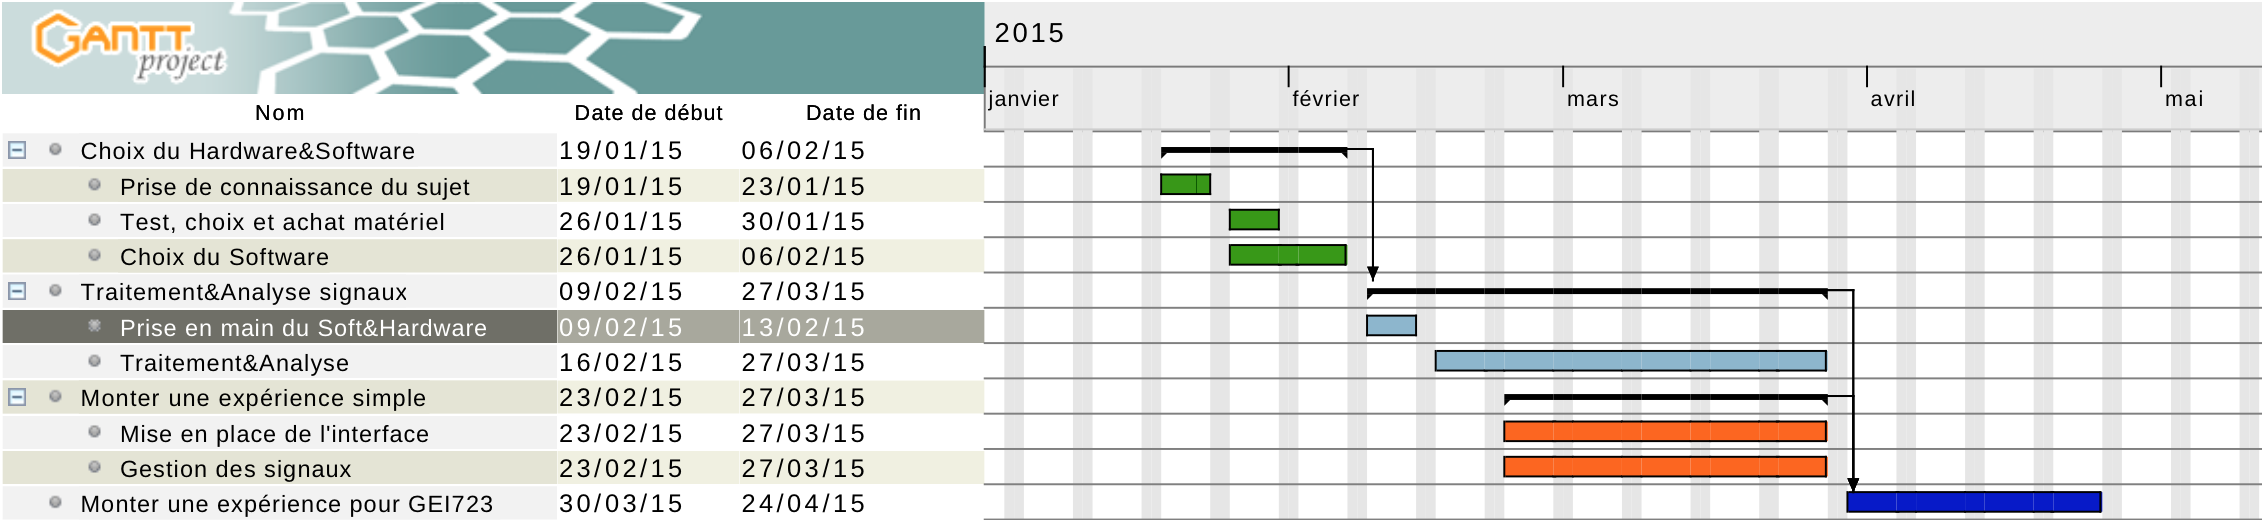
\includegraphics[width=15cm,height=6cm]{images/gant.png}
	\caption{Planning de Gantt prévisionnel}
\end{figure}

  \chapter{Neurophysiologie}
\label{Chapitre: Neurophysiologie}
\thispagestyle{fancy}

Le système nerveux est un ensemble de structures complexes permettant à un animal d'interagir avec les différentes parties de son corps, ainsi qu'avec son environnement extérieur. Celui de l'Homme est composé de deux structures  :

\smallbreak
\begin{itemize}
	\item Le Système Nerveux Central (SNC). Centre de décision, Il est composé du cerveau et de la moelle épinière. 
	\smallbreak
	\item Le Système Nerveux Périphérique (SNP). Il est constitué de nerfs et de ganglions, qui ont pour rôle de connecter les muscles ainsi que les structures éfferentes au Système Nerveux Central (SNC). Il est également composé de centres de décision autonomes, on parle alors de système nerveux autonomes (exemple : le système nerveux sympathique gérant de nombreuses activités dites inconscientes, comme le rythme cardiaque). 
\end{itemize}
\smallbreak
Nous nous intéressons plus particulièrement au SNC, les interfaces cerveau-ordinateur étant effectuées à partir de l'étude des signaux produits par le cerveau. 

\section {Cartographie du cerveau humain}
\label{Section: 2.Cartographie du cerveau humain}

Le cerveau humain est constitué de 2 éléments : l'aire corticale (elle même composée des lobes externes) et une partie interne, (composée des lobes limbiques) \cite{mcGill}. 

\subsection{Lobes externes}
\label{Subsection: 2.Lobes externes}
Le cortex cérébral est constitué de deux hémisphères : un hémisphère droit et un hémisphère gauche (souvent appelé cerveau droit et cerveau gauche) contrôlant l’ensemble de nos fonctions cognitives : mouvements volontaires, pensée, mémoire, etc. D’une manière générale, l’hémisphère droit commande le côté gauche du corps et inversement. (Figure \ref{test})

\begin{figure}[h]
	\centering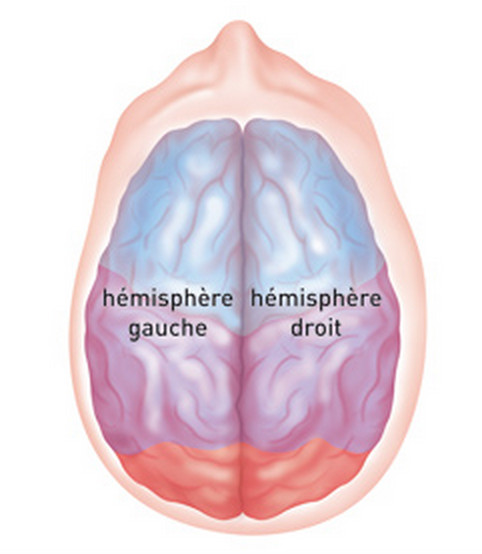
\includegraphics[width=5cm]{images/brainMap2.png}
	\caption[Les deux hémisphères du cerveau]{Les deux hémisphères du cerveau.\\Source : http://intelligences.livehost.fr/}
	\label{test}
\end{figure}

Chaque hémisphère est partagé en quatre lobes : le lobe frontal, le lobe pariétal, le lobe temporal et le lobe occipital (Figure \ref{fig:brainmap2}).

Chaque lobe gère différentes fonctions :

\begin{itemize}
	\item Les lobes frontaux : parole et langage, raisonnement, mémoire, prise de décision, personnalité, jugement, mouvements.
	\smallbreak
	\item Les lobes pariétaux : lecture, repérage dans l’espace, sensibilité.
	\smallbreak
	\item Les lobes occipitaux : vision.
	\smallbreak
	\item Les lobes temporaux : langage, mémoire, émotions.
\end{itemize}
\smallbreak
Le cortex cérébral est l'élément du cerveau humain qui le différencie des autres espèces animales. Elle regroupe 75\% des 100 milliards de neurones que possède l'être humain. 

\begin{figure}[h]
	\centering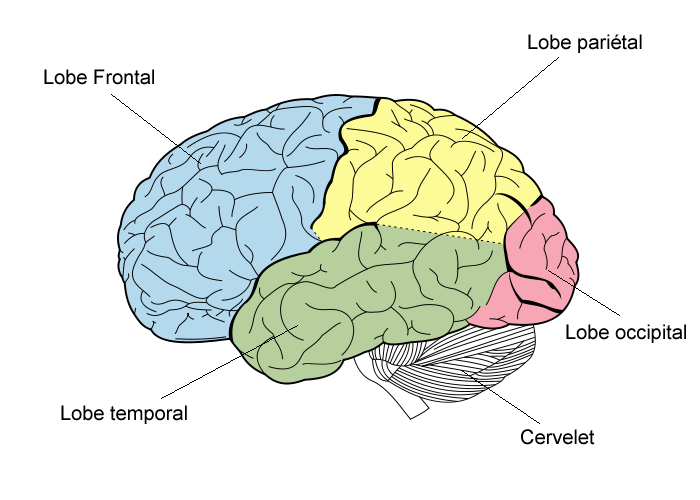
\includegraphics[width=8cm]{images/brainMap1.png}
	\caption[Représentation des différents lobes du cerveau]{Représentation des différents lobes du cerveau\\Source : http://commons.wikimedia.org/wiki/File:Lobes\_of\_the\_brain\_NL.svg?uselang=fr }
	\label{fig:brainmap2}
\end{figure}

\subsection{Lobes limbiques}
\label{Subsection: 2.Lobes limbiques}

Les lobes limbiques sont les élements du cerveau qui ne sont visibles que lorsque l'on en réalise une coupe. (Figure \ref{fig:limbique})
En voici la liste, ainsi que leurs principales fonctions : 

\begin{itemize}
	\item \textbf{Tronc cérébral}. Responsable des rythmes biologiques (respiration, rythme cardiaque, etc.).
	\smallbreak
	\item \textbf{Hippocampe}. Mémoire et navigation spatiale. 
	\smallbreak
	\item \textbf{Amygdale}. Régulation des émotions et apprentissage. 
	\smallbreak
	\item \textbf{Thalamus}. Relais et intégration des informations sensorielles (touché, vision, audition, goût).
	\smallbreak
	\item \textbf{Ganglions de la base}. Jouent un rôle dans le contrôle des mouvements. 
	\smallbreak
	\item \textbf{Hypothalamus}. Responsable de l'équilibre intérieur, c'est-à-dire les sensations de soif, de faim, la température corporelle, la sécrétion d'hormones, etc. 
	\smallbreak
	\item \textbf{Circonvolution cingulaire}. Ajuste certains paramètres corporels en fonction des émotions (pression sanguine, taille des pupilles, etc.)
	\smallbreak
	\item \textbf{Corps calleux}. Relie les deux hémisphères du cortex cérébral. 
	\smallbreak
	\item \textbf{Cervelet}. Joue un rôle essentiel dans le contrôle moteur.
\end{itemize}

\smallbreak
\begin{figure}[h]
	\centering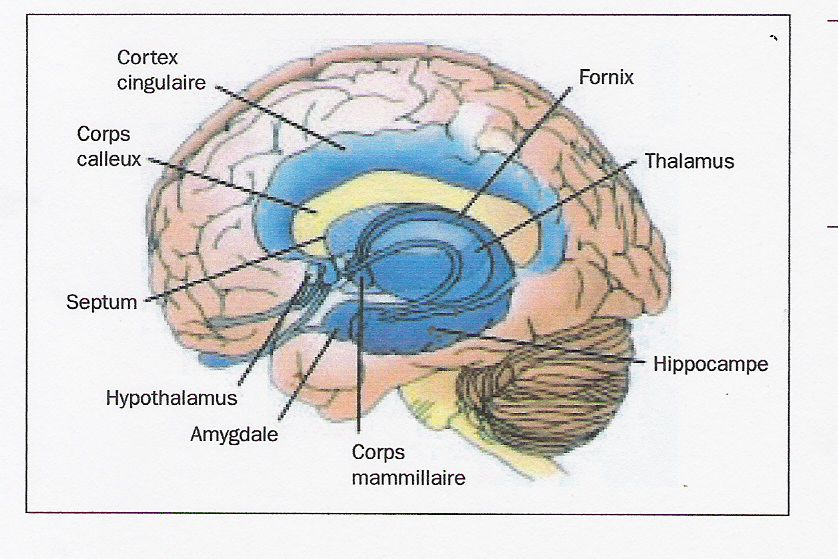
\includegraphics[width=11cm]{images/lobesLimbiques.jpg}
	\caption[Système limbique du cerveau humain.]{Système limbique du cerveau humain.\\Source : http://lucebarrault-psy.wifeo.com/article-73000-le-systeme-emotionnel.html}
	\label{fig:limbique}
\end{figure}

\section {Activité neuronale et potentiel d'action}
\label{Section: 2.Activité neuronale et potentiel d'action}

Le système nerveux est constitué de cellules nerveuses et de cellules gliales, situées entre les neurones. Chaque cellule nerveuse est composée de trois éléments : l'arbre dendritique, la synapse et le corps cellulaire (ou soma) (Figure \ref*{fig:structure d'un neurone}). Celles-ci répondent à des stimuli et envoient des informations vers d'autres neurones. L'axone est un long cylindre transmettant des impulsions électriques. Chaque dendrite est connectée aux axones ou aux dendrites d'autres neurones (environ 10 000), formant ainsi un réseau neuronal. La zone de connexion entre une dendrite et un axone est appelée la synapse. Le neurone post-synaptique reçoit alors de la part du neurone pré-synaptique une impulsion, puis la relaie à d'autres cellules nerveuses. L'activité neuronale du cerveau est en partie liée aux courants électriques échangés au niveau des synapses. Sans activité synaptique, on mesure un potentiel membranaire de -70mV au niveau du neurone, on dit qu'il est au repos. Ce potentiel membranaire change en fonction de l'activité des synapses. Si celui-ci dépasse un certain seuil, le neurone va alors émettre un potentiel d'action vers un neurone post-synaptique \cite{Saeid}.

\begin{figure}[h]
	\centering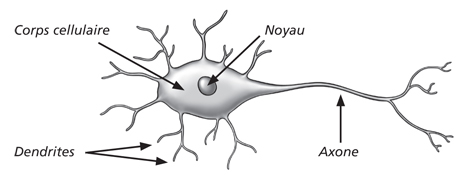
\includegraphics[width=11cm,height=4cm]{images/neurone.jpg}
	\caption[Structure d'une cellule neuronale]{Structure d'une cellule neuronale\\Source : http://www.thierrysouccar.com/bien-etre/info/comment-fonctionne-le-cerveau-386}
	\label{fig:structure d'un neurone}
\end{figure}


\section {Signaux EEG et rythmes du cerveau}
\label{Section: 2.Signaux EEG et rythmes du cerveau}

Un signal électroencéphalographique (ou signal EEG) correspond au champ électrique créé lors des échanges de courant entre les différents neurones du cerveau, au niveau des synapses. Celui-ci est mesurable au niveau de la boite crânienne grâce à des électrodes. Lors d'un EEG, on observe plusieurs signaux caractéristiques (ou ondes cérébrales). Elles correspondent à un état cognitif particulier du cerveau, i.e. l'activité physique ou intellectuelle de l'individu. Elles sont décomposées en fonction de leur domaine fréquentiel \cite{Saeid} :

\begin{itemize}
	\item \textbf{<4 Hz : Ondes Delta.}
	Elles sont généralement associées à un sommeil profond ou à certains cycles du sommeil. 
	\smallbreak
	\item \textbf{4-8 Hz : Ondes Thêta}.
	Ces ondes sont la plupart du temps liées à l'état de somnolence d'un individu, la méditation profonde, la créativité et dans un cadre plus général à tout ce qui se rapporte à l'inconscience. C'est pour cela que le changement de rythme des ondes thêta est souvent observé lorsque l'on étudie l'activité émotionnelle d'une personne.
	Ces ondes proviennent la plupart du temps de l'activité du thalamus. 
	\smallbreak
	\item \textbf{9-14 Hz : Ondes Alpha}.
	Elles caractérisent un état de conscience dans lequel un individu est dans une phase de "relaxation". Se sont les ondes les plus courantes dans le cerveau. Elles proviennent en général de la région occipitale du cortex.
	\smallbreak
	\item \textbf{15-30 Hz : Ondes Bêta}.
	Ces ondes sont liées à l'état d'éveil du cerveau, notamment lorsqu'une personne est dans un état de réflexion ou d'attention important. Ces signaux sont en général observés dans la région frontale et centrale du cortex. 
	\smallbreak
	\item \textbf{>30 Hz : Ondes Gamma}.
	Elles sont associées à certaines actions motrices du corps humain et sont généralement observées au niveau de la zone frontale du cortex. 
\end{itemize}

\smallbreak

Dans le cadre de notre projet, nous nous interesserons essentiellement aux ondes alpha et bêta.

  \chapter{Choix du matériel et du logiciel}
\label{Chapitre:Choix du Hardware et du Software}
\thispagestyle{fancy}

\section{Méthodes d'enregistrement d'un signal EEG}
\label{Section:3.Méthodes d'enregistrement d'un signal EEG}

Il existe deux types de systèmes électroencéphalographiques :
\smallbreak
\begin{itemize}
	\item \textbf{Les EEG intracrâniens}. Il s'agit de systèmes dits invasifs : on vient enregistrer l'activité neuronale du cerveau en implantant des électrodes directement dans la boite crânienne. Bien que cette technique offre des résultats probants, elle nécessite une intervention chirurgicale, ce qui n'est pas réalisable dans le cadre de notre projet. 
	\smallbreak
	\item \textbf{Les EEG de scalpe (ou de surface)}. Ce système étudie les variations du courant diffusé par le cerveau sur la surface du crâne. Il s'agit d'un système non invasif et c'est en toute logique que nous utiliserons ce type de dispositif.

\end{itemize}
\smallbreak
La visualisation et l'enregistrement d'un signal EEG passe donc par l'utilisation d'électrodes. Il s'agit de capteurs sensibles aux variations du champ électrique générées par les échanges électriques entre les neurones. Le signal EEG est atténué par des éléments physiques comme le crâne ou la peau, il doit donc être amplifié afin d'être visualisé et traité. Du bruit est également observé lors de l'acquisition de signaux EEG. Celui-ci provient à la fois du cerveau et de l'environnement extérieur. 

\begin{figure}[h]
	\centering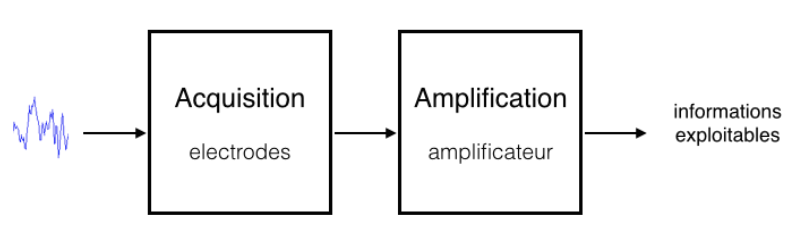
\includegraphics[width=14cm]{images/chaineSignal.png}
	\caption{Chaine d'acquisition d'un signal EEG}
	\label{fig:GRASS}
\end{figure}

\section{Caractéristiques générales du matériel}
\label{Section:3.Caractéristiques générales du matériel}

\subsection{Électrodes}
\label{Subsection:3.Électrodes}

Il existe différents types d'électrodes :
\smallbreak
\begin{itemize}
	\item \textbf{Les électrodes jetables}.
	\smallbreak 
	\subitem - \textbf{Les électrodes sèches.} Se sont les plus simples à utiliser car elles ne nécessitent pas l'utilisation de gel pour réaliser le contact avec la peau. Elles sont cependant moins précises que des électrodes à gel.
	\smallbreak
	\subitem - \textbf{Les électrodes à gel}. Ce type d'électrode utilise un gel afin d'améliorer le contact entre l'électrode et la surface du crâne.  
	\smallbreak
	\item \textbf{Les électrodes réutilisables}. Elles sont constituées de matériaux conducteurs permettant de capter les courants présents. Différents matériaux peuvent être utilisés (or, acier inoxydable, argent, etc.), chacun possédant une qualité de conduction plus ou moins élevée. 
	\smallbreak
	\item \textbf{Les casques à électrodes}. Ce sont les dispositifs les plus utilisés en R\&D. Ils offrent une stabilité accrue vis à vis du placement des électrodes et évitent ainsi l'introduction de bruits.
	\smallbreak
	\item \textbf{Les électrodes à aiguilles}. Il s'agit d'électrodes possédant une partie sous-cutanée. Elles offrent de bons résultats mais la pose nécessite l'assistance d'un médecin.
\end{itemize}
\smallbreak
Après étude des avantages et des inconvénients des différents systèmes, notre choix se porte sur l'utilisation d'un casque à électrodes. 

Plus le nombre d'électrodes utilisées est élevé, plus la qualité de l'information spatiale sera importante. Le placement des électrodes de surface au niveau de la boîte crânienne répond au standard "International 10-20 System" (Figure \ref{fig:InternationalSystem}). Chaque zone du cerveau est donc scrutée par une électrode. On parle alors de canal. (exemple : O1 correspond au canal analysant par la partie occipitale gauche du cortex, O2 la partie droite).

\begin{figure}[h]
	\centering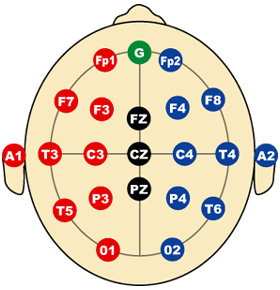
\includegraphics[width=6cm]{images/electrodesStandard.png}
	\caption[Standard International 10-20 System à 23 électrodes.]{Standard International 10-20 System à 23 électrodes\\Source : https://tel.archives-ouvertes.fr/tel-00822833/document}
	\label{fig:InternationalSystem}
\end{figure}

\subsection{Amplificateur}
\label{Subsection:3.Amplificateur}

L'amplificateur effectue deux tâches : l'amplification des signaux EEG et leur échantillonnage. Certains amplificateurs proposent également de réaliser un filtrage temporel. Nous souhaitons cependant l'implémenter par nos propres moyens dans ce projet. Un amplificateur est caractérisé par : 
\smallbreak
\begin{itemize}
	\item Son gain.
	\smallbreak
	\item Son taux d'échantillonnage.
	\smallbreak
	\item Sa résolution numérique.
	\smallbreak
	\item Son ratio signal sur bruit. 
\end{itemize}
\smallbreak
Il existe des amplificateurs directement intégrés dans le casque EEG, cependant leur qualité reste moindre que les systèmes conventionnels. Leur usage est principalement destiné aux jeux vidéos et n'est pas adapté à la réalisation d'examens médicaux. 

\section {Choix du matériel}
\label{Section:3.Choix du matériel}
Pour ce projet, nous disposons du matériel suivant :
\smallbreak
\begin{itemize}
	\item Le casque biopac CAP100C, composé de 19 électrodes à gel \cite{biopac} (Figure \ref{fig:CAP100C}).
	\smallbreak
	\item L'amplificateur 15LT de Grass Technologies. Il s'agit d'un amplificateur de 16 canaux. Il est utilisable à la fois pour les EEG, les EMG et les ECG. Celui-ci est fournit avec un logiciel propriétaire, GrassLab, permettant l'acquisition et l'exportation des données \cite{grass} (Figure \ref{Grass}).
\end{itemize}

\smallbreak

\begin{figure}[h]
	\centering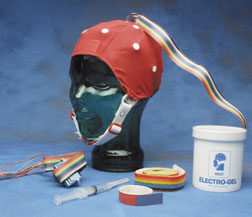
\includegraphics[width=7cm]{images/cap100.jpg}
	\caption[CAP100C de Biopac]{CAP100C de Biopac.\\Source : http://www.biopac.com/BioNomadix-EEG-CAP-medium}
	\label{fig:CAP100C}
\end{figure}

\begin{figure}[h]
	\centering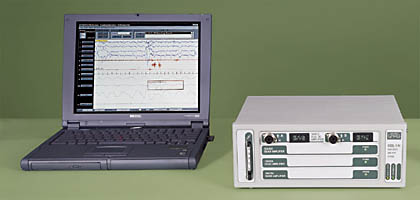
\includegraphics[width=10cm]{images/GRASS.jpg}
	\caption[GRASS amplifier 15LT]{GRASS amplifier 15LT.\\Source : http://www.grasstechnologies.com/products/ampsystems/15lt.html}
	\label{Grass}
\end{figure}

Pour commencer, nous avons utilisé le CAP100C de Biopac avec l'amplificateur GRASS. Nous avons pu observer les différents signaux EEG (concentration, calcul mental simple, repos, lecture, etc). Notre objectif étant de réaliser une interface cerveau-ordinateur dans un cadre pédagogique, ce matériel ne semble pas adapté pour plusieurs raisons :
\smallbreak
\begin{itemize}
	\item Casque et amplificateur Grass onéreux (difficile d'en avoir plusieurs exemplaires)
	\smallbreak
	\item Logiciel propriétaire GrassLab obsolète, le support technique n'est plus assuré.
	\smallbreak
	\item Confort d'utilisation du casque discutable.
	\smallbreak
	\item Le produit s'adresse essentiellement au marché médical.
\end{itemize}
On souhaite acquérir un autre système EEG plus adapté à l'utilisation dans le cadre d'un cours. Une étude comparative de différents produits du marché est proposée (Voir le tableau présenté en annexe). D'après l'analyse comparative, notre choix se porte sur la gamme de produit de la marque Emotiv. En effet, le prix des produits est attractif pour les performances proposées, et est cohérent avec notre budget. Voici un tableau qui présente les principales différences entre les 3 casques de la marque.

\begin{figure}[h]
	\centering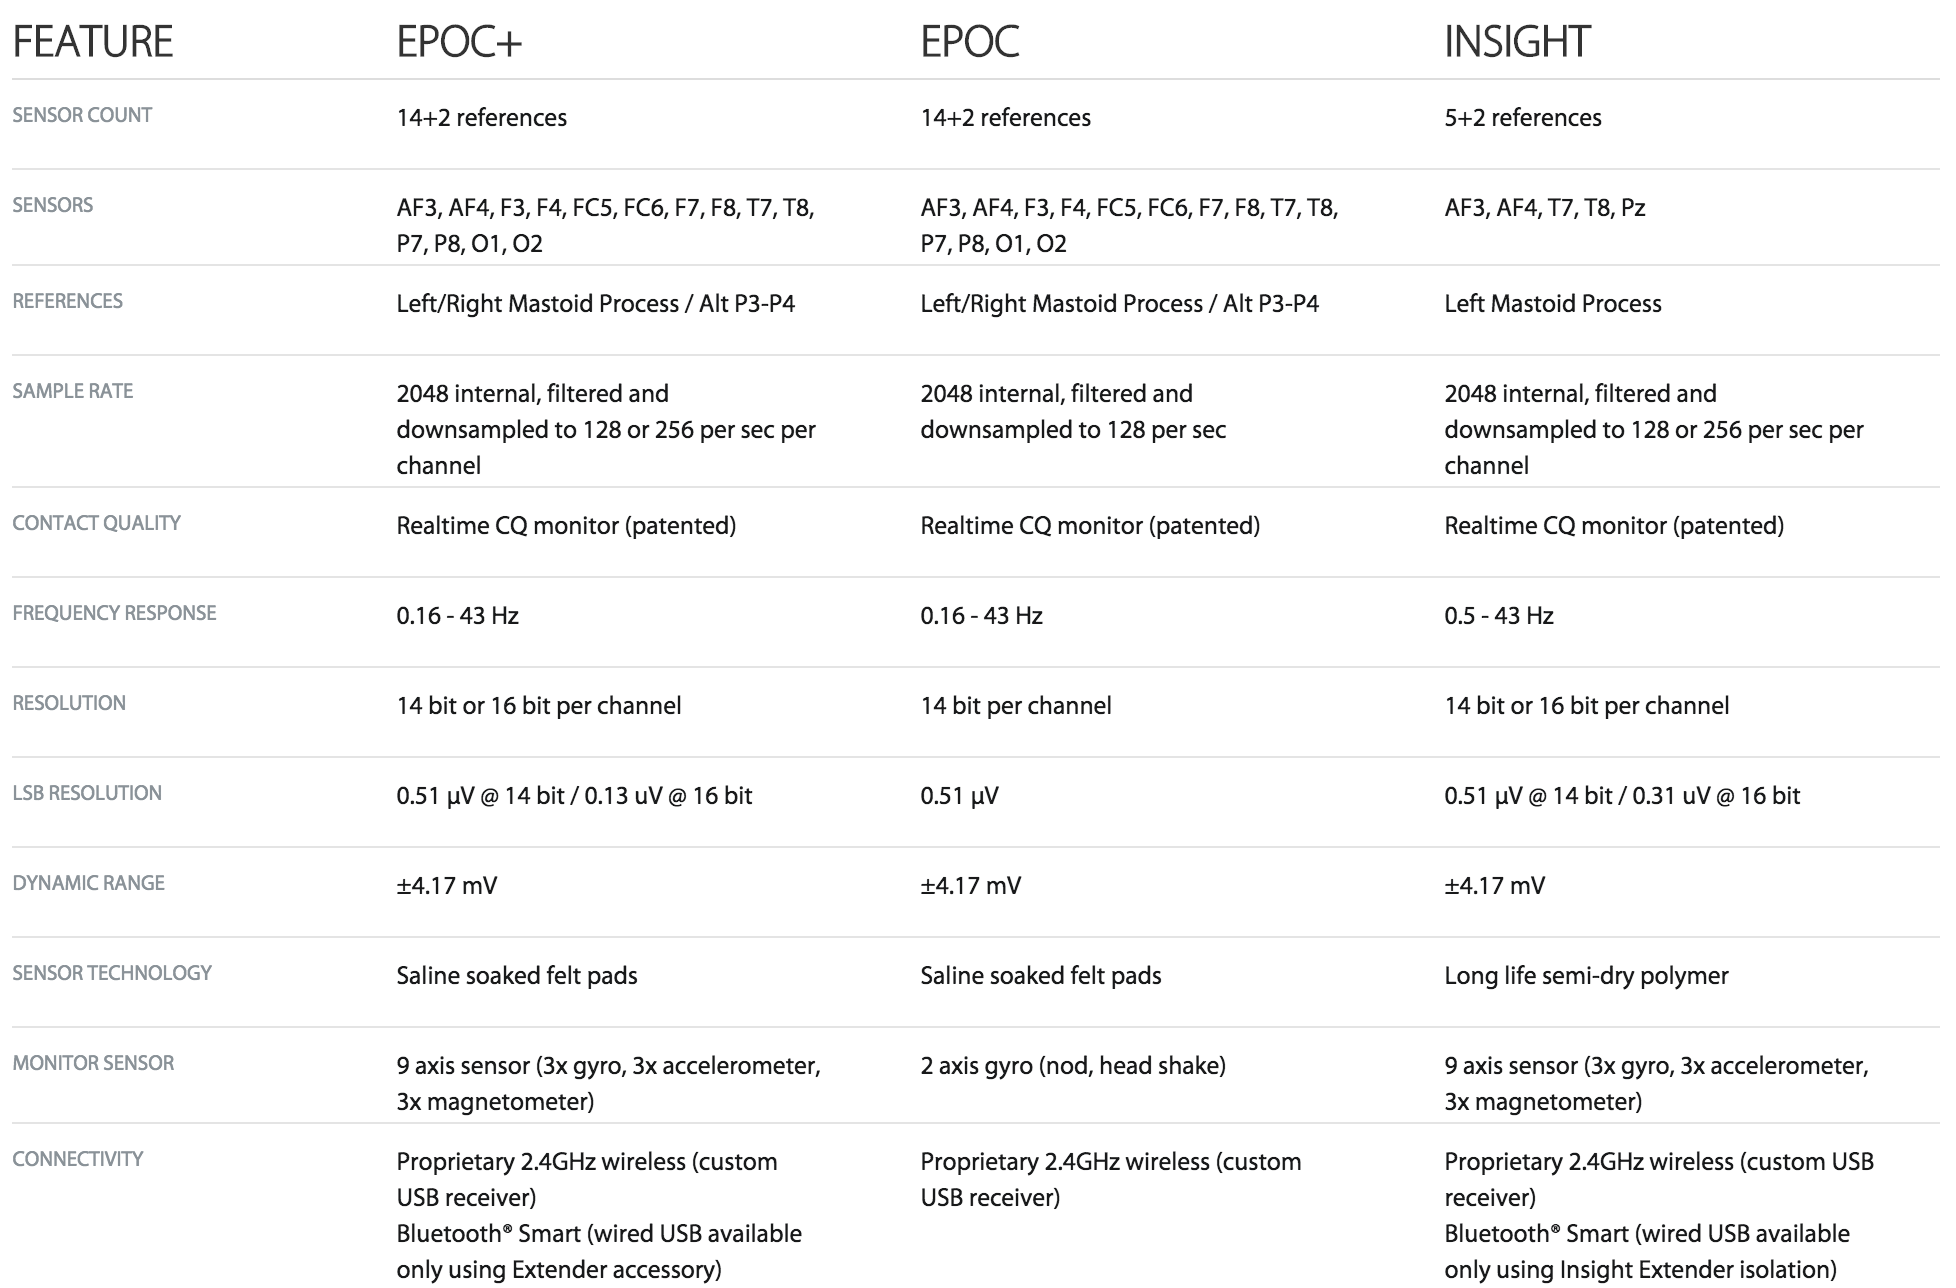
\includegraphics[width=15cm,height=15cm]{images/emotiv_comparaison.png}
	\caption[Comparaison entre les différents casques Emotiv]{Comparaison entre les différents casques Emotiv \\Source : http://emotiv.com}
	\label{fig:Emotiv_Comparaison}
\end{figure}

Le casque Emotiv INSIGHT n'est pas assez performant pour nos travaux et convient plus pour des activités vidéoludiques (iI ne dispose que de 5 capteurs). En revanche, les casques EPOC et EPOC+ semblent plus adaptés \cite{epoc}. Il est possible d'accéder aux données EEG brutes, à condition d'acquérir une licence SDK. 
Après étude des produits, nous proposons à l'université de Sherbrooke d'acquérir le casque EPOC.
 Voici le devis : 
\begin{itemize}
	\smallbreak
	\item Casque : 399\$US;
	\smallbreak
	\item SDK "licence de recherche individuelle" : 300\$US.
	\smallbreak
	\item Licence supplémentaire Mac OS X : 90 \$US.
	\smallbreak
	\item Total : 789\$US.
\end{itemize}

\begin{figure}[h]
	\centering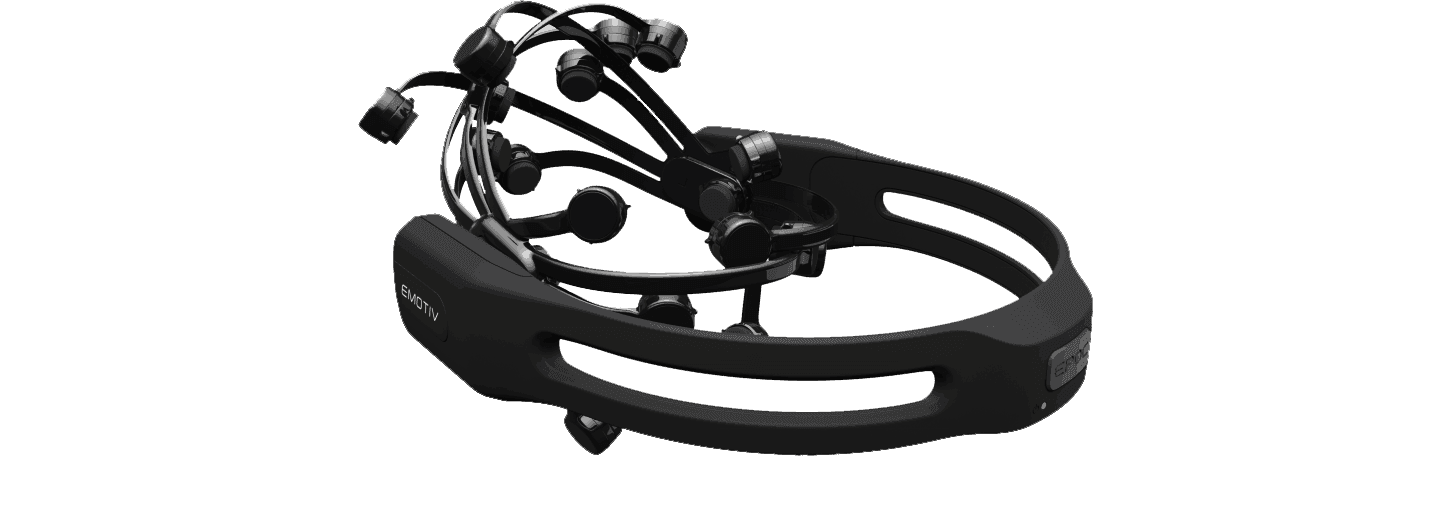
\includegraphics[width=12cm]{images/EPOC.png}
	\caption[EPOC headset - Emotiv]{EPOC headset - Emotiv.\\ Source : http://emotiv.com}
	\label{fig:EPOC}
\end{figure}

\section {Choix du logiciel}
\label{Section:3.Choix du logiciel}
Il existe principalement deux logiciels libres de droit, compatibles avec le casque EPOC : EEGLAB et OpenViBE (Open Virtual Brain Environment).
\smallbreak
EEGLAB fonctionne avec l'outil Simulink de Matlab. Il est majoritairement utilisé pour le traitement du signal. Il nécessite cependant l'acquisition d'une licence Matlab pour chaque poste de travail, ce qui peut s'avérer onéreux dans le cadre d'un cours suivi par plusieurs étudiants.
\smallbreak
OpenVIBE propose quant à lui sa propre interface (i.e. fonctionne sans logiciel tiers). Il est majoritairement utilisé dans le développement de liaisons cerveau-ordinateur. Celui-ci est gratuit, fonctionnel avec le casque EPOC, bien documenté et performant. Il fonctionne de plus sur les plateformes Windows et Linux. Ce logiciel a été développé par l'équipe de l'Institut National de Recherche en Informatique et Automatique (INRIA) de Rennes en France.
  \chapter{Traitement des signaux EEG}
\label{Chapitre : Traitement des signaux EEG}
\thispagestyle{fancy}

Le schéma conceptuel en annexe présente les différentes méthodes de traitement et d'analyse des signaux EEG, ainsi que les différentes interfaces cerveau-ordinateur existantes. 

\section{Caractéristiques des signaux étudiés}
\label{Section : 4.Caractéristiques des signaux étudiés}

\begin{figure}[h]
	\centering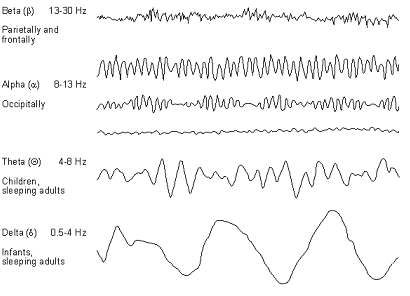
\includegraphics[width=12cm]{images/rythmesCerveau.png}
	\caption[Signaux des différents rythmes du cerveau]{Signaux des différents rythmes du cerveau.\\Source : http://www.computer.org/csdl/proceedings/bibe/2012/4357/00/06399691.pdf}
\end{figure}

A partir des rythmes du cerveau, il est possible d'extraire différentes informations, dont les 3 plus utilisées sont : 

\begin{itemize}
	\item \textbf{Information spectrale}. Variations la puissance du signal dans certaines bandes de fréquences.
	\smallbreak
	\item \textbf{Information temporelle}. Variations du signal en fonction du temps. 
	\smallbreak
	\item \textbf{Information spatiale}. Position d'une source. Pour obtenir cette information, on doit faire appel à plusieurs signaux EEG, en utilisant plusieurs électrodes.  
\end{itemize}

\section{Différentes interfaces cerveau-ordinateur}
\label{Section : 4.Différents types d'interfaces cerveau-ordinateur}

Il existe plusieurs types d'interfaces cerveau-ordinateur, les deux principales sont :
\smallbreak
\begin{itemize}
	\item Celles basées sur les activités oscillatoires. 
	\smallbreak
	\item Celles basées sur les potentiels évoqués. 
\end{itemize} 
\smallbreak
\subsubsection{Liaisons cerveau-ordinateur basées sur les activités oscillatoires}
\label{Subsection : 4.Liaisons cerveau-ordinateur basées sur les activités oscillatoires}

Il s'agit de la méthode la plus couramment utilisée. Elle consiste en l'étude des variations de la puissance sur certaines bandes de fréquence, en fonction des changements d'états mentaux de certaines zones du cerveau. Elle exploite donc l'information spatiale et spectrale. L'activité oscillatoire d'un signal EEG peut être caractérisée par deux évènements (Figure \ref{ers}):
\smallbreak 
\begin{itemize}
	\item \textbf{ERS, Synchronisation des événements liés}. Diminution de l'énergie due à l'activation corrélée du système nerveux dans certaines aires corticales.
	\smallbreak
	\item \textbf{ERD, Désynchronisation des événements liés}. Augmentation de l'énergie due à la désactivation corrélée du système nerveux dans certaines aires corticales.
\end{itemize} 
\smallbreak
Ces phénomènes oscillatoires sont essentiellement observés dans les rythmes alpha et bêta du cerveau.

\begin{figure}[h]
	\centering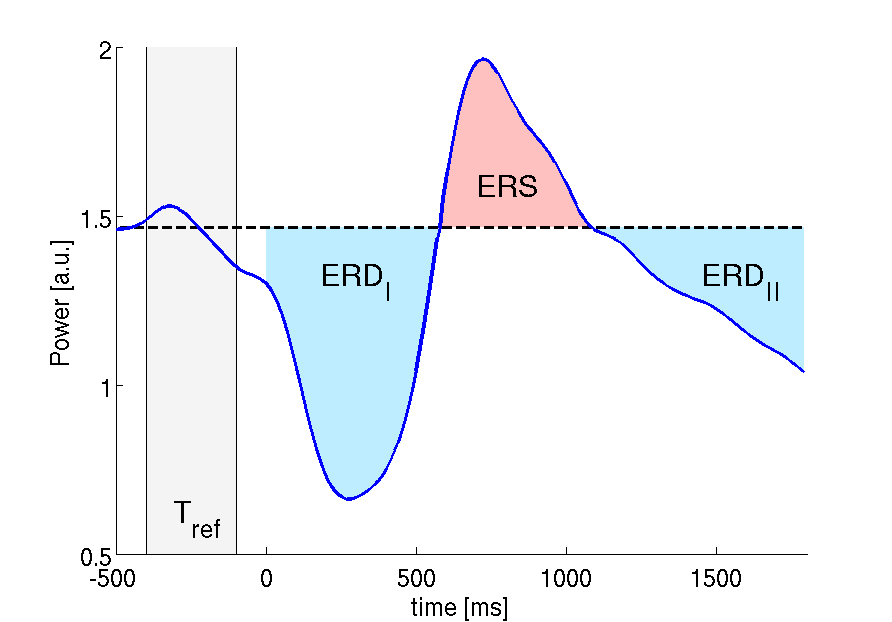
\includegraphics[width=10cm]{images/ERS_ERD.png}
	\caption[Représentation des phénomènes d'oscillations ERS et ERD du rythme bêta du cerveau]{Représentation des phénomènes d'oscillations ERS et ERD du rythme bêta du cerveau.\\Source : http://www.bbci.de/supplementary/conditionalERD/conditionalERD.htm}
	\label{ers}
\end{figure}

Les interfaces cerveau-ordinateur qui s'appuient sur les activités oscillatoires du cerveau sont principalement employées dans des dispositifs s'appuyant sur des stimulations visuelles, ou lorsqu'on fait appel à la représentation et à la visualisation mentale d'objets en mouvement. Voici les deux interfaces cerveau-ordinateur basées sur les activités oscillatoires les plus utilisées : 
\smallbreak
\begin{itemize}
	\item \textbf{SSVEP - Potentiel évoqué visuellement}. Ce dispositif repose sur une stimulation visuelle \cite{SSVEP}. En effet, lorsque la rétine est excitée par une stimulation ayant une certaine fréquence (généralement entre 3.5 Hz et 75 Hz), le cerveau génère des signaux électriques (les SSVEP) de même fréquence que le stimulus. Cette méthode a l'avantage de nécessiter une période d'entrainement relativement courte (Figure \ref{SSVEP}).
	\smallbreak
	\item \textbf{Imagerie motrice}. Ce système repose quant à lui sur des méthodes d'entrainement à l'imagination mentale, i.e. on demande à un individu de penser à une action, comme bouger un cube dans un espace en 3 dimensions \cite{motor}. On observe alors des fluctuations dans les rythmes du cerveau que l'on pourra par la suite interpréter, et en déduire l'action pensée par la personne. L'inconvénient de cette méthode est qu'elle nécessite plusieurs sessions d'entrainement. Elle n'exige cependant pas de stimulation visuelle. 
\end{itemize}
\smallbreak
\begin{figure}[h]
	\centering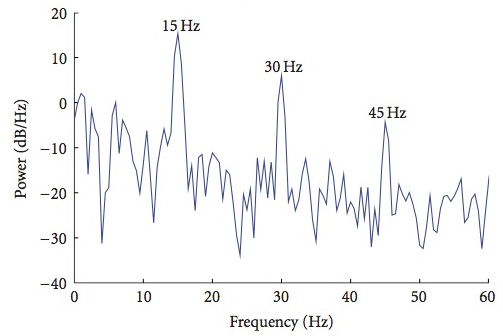
\includegraphics[width=10cm]{images/SSVEPSIgnal.jpg}
	\caption[Signal EEG de type SSVEP, en réponse à une stimulation visuelle de 15Hz]{Signal EEG de type SSVEP, en réponse à une stimulation visuelle de 15Hz.\\Source : http://www.hindawi.com/journals/cin/2010/702357/fig2/}
	\label{SSVEP}
\end{figure}

\subsubsection{Liaisons cerveau-ordinateur basées sur les potentiels évoqués}
\label{Subsection : 4.Liaisons cerveau-ordinateur basées sur les potentiels évoqués}

Il s'agit d'une méthode qui s'appuie sur l'étude  de l'information temporelle et spatiale des signaux EEG du cerveau \cite{p300}. Ce dispositif étudie les potentiels à évenements liés (ERP). Il s'agit de signaux émis par le cerveau lorsque celui-ci est excité par un stimulus (visuel, tactile, etc). Un des ERP les plus utilisé actuellement, et notamment dans le monde des jeux-vidéos est le P300. Il s'agit d'une déflexion positive qui intervient 300ms environ après la stimulation sensorielle (Figure \ref{P300}).

\begin{figure}[h]
	\centering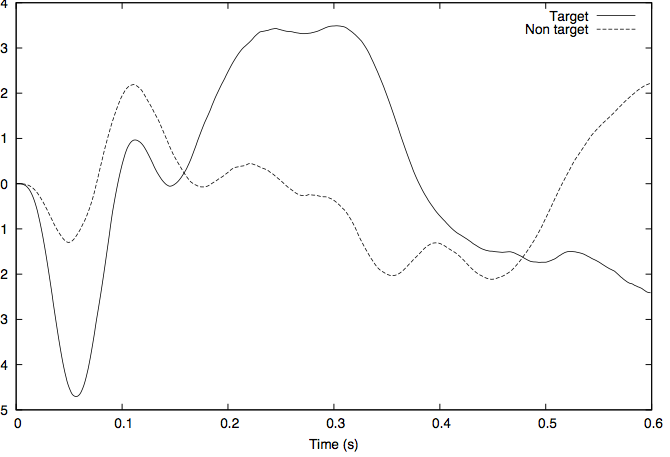
\includegraphics[width=9cm]{images/P300.png}
	\caption[Réponse P300]{Réponse P300 après un stimulus. On observe clairement la déflexion du signal après 300ms.}
	\label{P300}
\end{figure}

\section{Traitement et analyse des signaux EEG}
\label{Section : 4.Traitement et analyse des signaux EEG}

Le processus fonctionnel d'une interface cerveau-ordinateur peut être décrit comme un système en boucle fermée, composé de six étapes \cite{Saeid}\cite{Lotte} (Figure \ref{bci}) :

\begin{figure}[h]
	\centering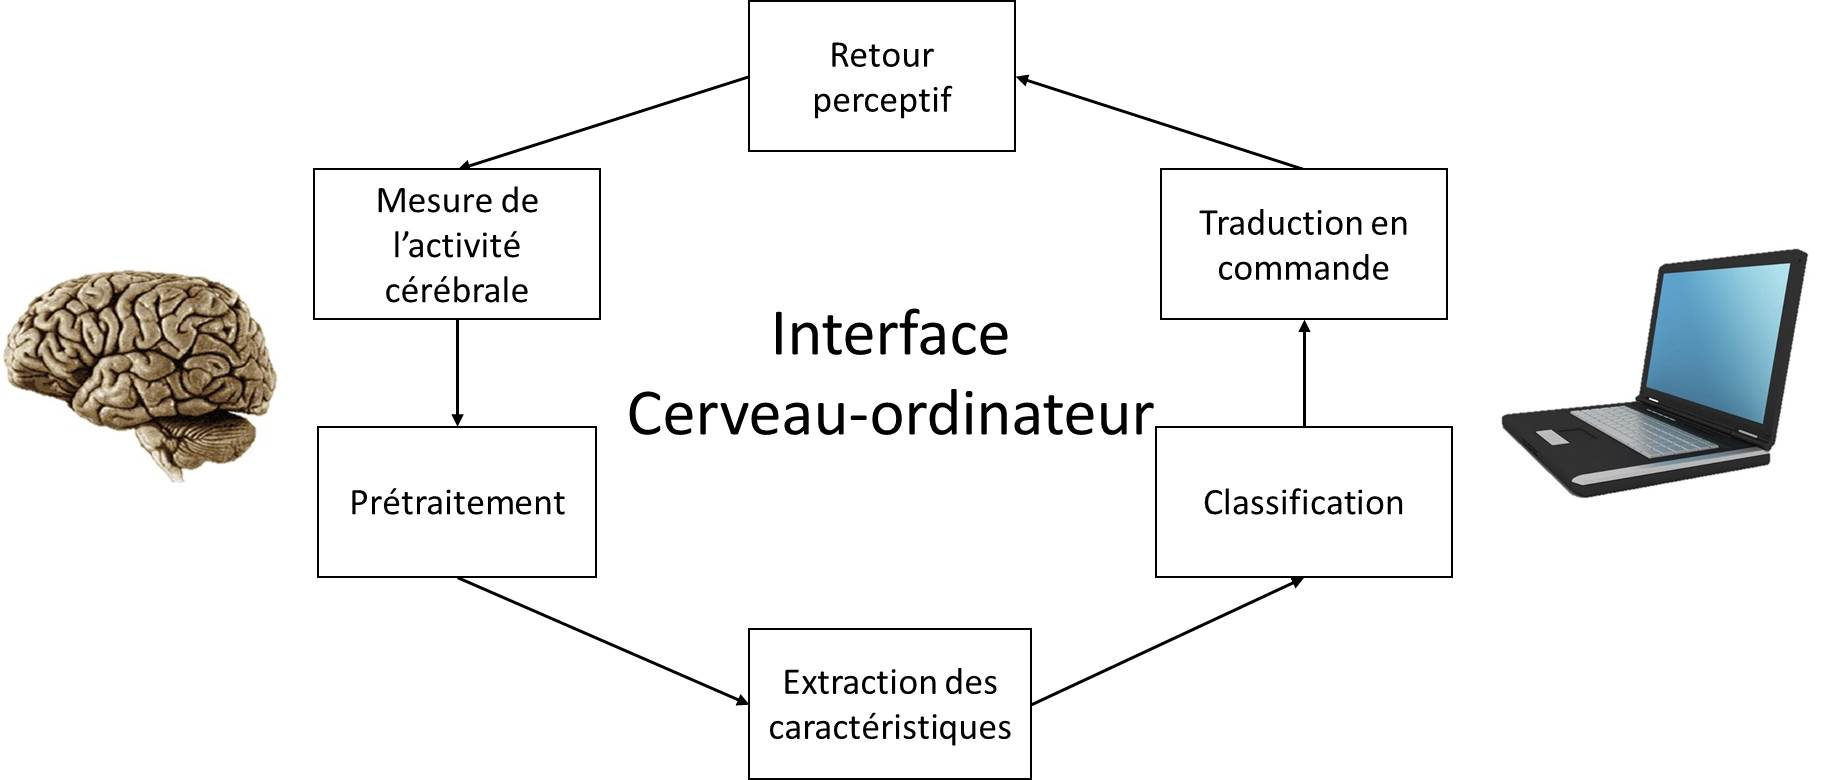
\includegraphics[width=15cm]{images/bci.jpg}
	\caption{Principales étapes constituant une interface cerveau-ordinateur.}
	\label{bci}
\end{figure}

\begin{enumerate}
	\item Mesure de l'activité cérébrale via un dispositif électroencéphalographique. On parle de phase d'acquisition des signaux. 
	\smallbreak
	\item Pré-traitement et filtrage des signaux cérébraux permettant notamment de dissocier les différents rythmes du cerveau. 
	\smallbreak
	\item Extraction des caractéristiques des signaux, afin de ne conserver que des informations pertinentes.
	\smallbreak
	\item Classification des signaux, afin d'identifier et de caractériser l'activité mentale et de l'interpréter. 
	\smallbreak
	\item Traduction en une commande envoyée à l'ordinateur. On fait ici le lien entre l'interprétation et la tâche qu'il doit effectuer.
	\smallbreak
	\item Retour perceptif. Il peut par exemple s'agir d'un retour visuel lié à l'activité neuronale perçue. L'utilisateur va ainsi progressivement apprendre à mieux contrôler le système, et ainsi boucler le synoptique de l'interface cerveau-ordinateur. 
\end{enumerate}

\smallbreak
On cherche ici a étudier le traitement et l'analyse des différents signaux EEG acquis grâce au casque EEG Emotiv. On s'intéressera principalement aux étapes 1, 2, 3 et 4. On a donc la chaîne de traitement suivante (Figure \ref{traitementEEG1}). 

\begin{figure}[h]
	\centering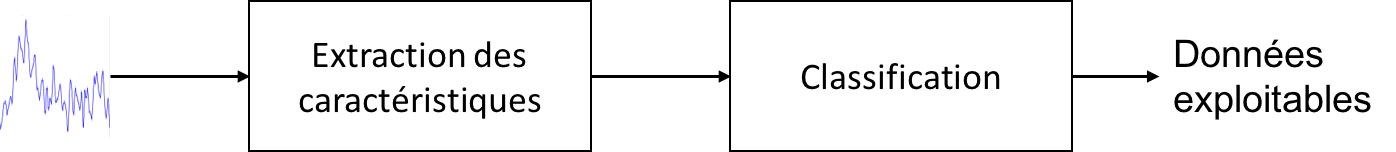
\includegraphics[width=16cm]{images/traitementEEG1.png}
	\caption{Chaine de traitement d'un signal EEG}
	\label{traitementEEG1}
\end{figure}

Cette trame est utilisée pour le traitement d'un seul signal, c'est-à-dire pour un signal provenant d'une seule électrode. Or, étudier le signal de plusieurs électrodes permet d'augmenter la précision du système. Cela permet également d'accéder à une information supplémentaire : la localisation spatiale des signaux. Ce type de procédé augmente inévitablement la quantité de calculs à effectuer, d'autant plus que les informations doivent être traitées en temps réel. Pour palier à ce problème, on ajoute une étape d'optimisation des données (prétraitement) afin de réduire le nombre d'informations à manipuler. On obtient donc cette nouvelle chaine de traitement (Figure \ref{traitementEEG2}) : 

\begin{figure}[h]
	\centering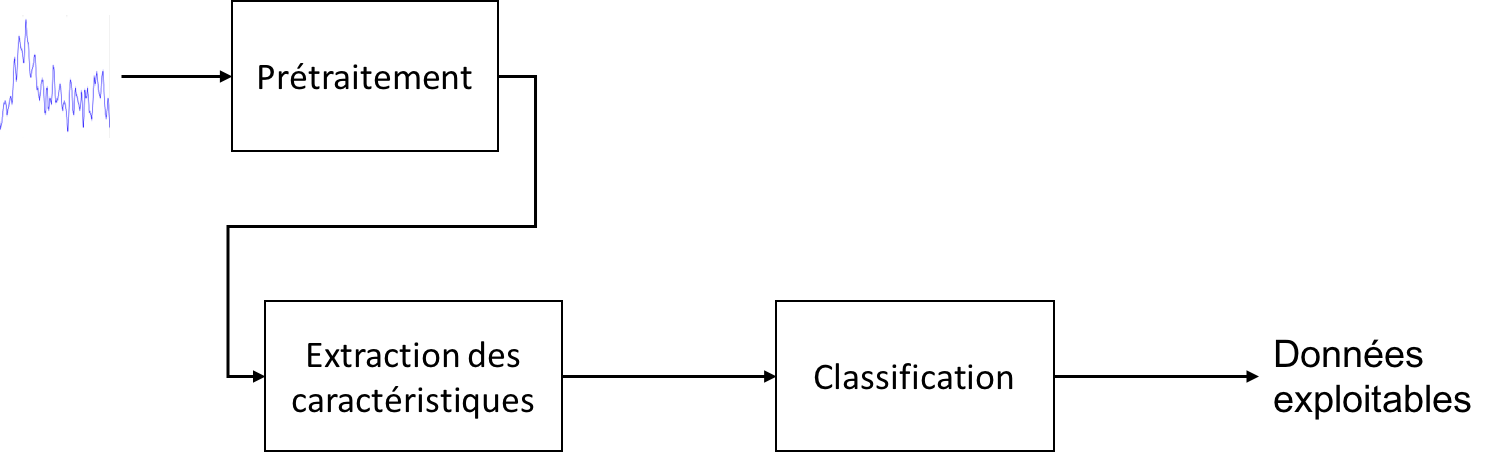
\includegraphics[width=14cm]{images/traitementEEG2.png}
	\caption{Chaine de traitement de plusieurs signaux EEG}
	\label{traitementEEG2}
\end{figure}

\subsection{Pré-traitement, méthodes d'optimisation des données}
\label{Subsecton : 4.Pré-traitement, méthodes d'optimisation des données}

Il existe différents algorithmes d'optimisation des données, afin de réduire la quantité d'informations à traiter en temps-réel \cite{Lotte}.
\smallbreak
\begin{itemize}
	\item \textbf{Sélection des caractéristiques.} Algorithme permettant de sélectionner automatiquement les données les plus pertinentes. 
	\smallbreak
	\item \textbf{Sélection des entrées (électrodes).} Sélectionne automatiquement les électrodes dont les données sont les plus pertinentes. Cet algorithme est en général plus efficace que les méthodes de sélection des caractéristiques.
	\smallbreak 
	\item \textbf{Filtrage spatial.} On réalise une combinaison lineaire des signaux issus des électrodes par suppression des redondances afin de réduire la quantité d'informations à traiter. 
\end{itemize}

\subsubsection{Filtrage spatial}
\label{Subsubsecton : 4.Filtrage spatial}
Le filtrage spatial permet de réduire la quantité d'informations à traiter en fusionnant des chaines entres elles \cite{Lotte} \cite{Saeid} . Il a également un sens du point de vu physiologique car il permet de retrouver les signaux sources. On définit donc le filtrage spatial comme une combinaison linéaire de l'ensemble des chaines, chaque chaine étant pondérée par un poids : 

\begin{equation}
		\tilde{x}=\sum{w_i*x_i}
\end{equation}

Où $\tilde{x}$ est le signal filtré spatialement, $i$ le canal traité, $w_i$ le poids attribué à $i$, $x_i$ le signal EEG de $i$.

Il existe plusieurs méthodes de filtrage spatial : 
\smallbreak
\begin{itemize}
	\item  \textbf{Filtrage spatial fixe.} Dans un filtrage fixe, le poids attribué à chaque canal est prédéterminé par l'utilisateur. On utilise cette méthode principalement pour réduire le bruit de fond. En voici deux couramment utilisées : 
	\smallbreak
	\subitem \textbf{Filtre Bipolaire.} On calcule la différence entre deux canaux à proximité du canal que l'on souhaite étudier : $ C_z = FC_3 - C_4 $, où $C_z$, $FC_3$ et $C_4$ correspondent au placement des électrodes selon la norme Internationale 10-20.
	\smallbreak
	\subitem \textbf{Filtre Laplacien.} $ C_z = 4C_z-F_z-P_z-C_3-C_4$. où $C_z$, $F_z$,$P_z$,$C_3$, et $C_4$ correspondent au placement des électrodes selon la norme Internationale 10-20.
	\smallbreak
	\item \textbf{Filtrage spatial avec apprentissage.} Les poids sont déterminés automatiquement, grâce à un d'apprentissage.
	\smallbreak
	\subitem\textbf{PCA, Analyse en composantes principales.} La PCA permet d'extraire des informations à partir de signaux bruités et de réduire le nombre de données à traiter.
	\smallbreak
	\subitem\textbf{ICA, Analyse en composantes indépendantes.} L'ICA est utilisée en BSS (Séparation des sources masquées), c'est-à-dire lors de l'extraction de sources à partir de plusieurs signaux (ex: identifier et extraire une voix dans une soirée à partir de plusieurs microphones).
	\smallbreak 
\end{itemize}

On s'intéressera ici plus particulièrement aux filtres spatiaux avec apprentissage car la sélection des poids à appliquer à chaque chaine est faite automatiquement.

\subsubsection{Analyse en composantes principales (PCA)}
\label{Subsubsecton : 4.PCA}
 C'est une méthode d'analyse statistique des données qui permet d'extraire certaines informations à partir d'un flot de données diffus. On réduit ainsi la complexité des données. Pour cela, on les exprime dans un nouveau repère en effectuant une transformation linéaire, afin de décorréler les données entres elles. Un flot de donnée peut être caractérisé par deux informations : le bruit et la redondance \cite{Lotte}.
 
 Soit $X$ une matrices contenant les échantillons de données de plusieurs sources ($m$x$n$, $m$ correspondant aux différentes sources $X_i$ avec $0<i<m$, $n$ aux valeurs des sources à chaque instant $t$ avec $0<j<n$), $Y$ la ré-écriture de $X$ dans le nouveau repère. On cherche donc à déterminer la transformation linéaire $P$ permettant de réduire à la fois le bruit et la redondance des données  \cite{PCA}, tel que 
 \begin{equation}
 	 Y = PX
 \end{equation}

 Avec :
   
   \begin{equation}
   \begin{blockarray}{cccccc}
   & t_1 & t_2 & t_3 & ... & t_{fin} \\
   \begin{block}{c(ccccc)}
   X_1 &  &  &  &  &  &  \\
   X_2 &  &  &  &  &  &  \\
   X_3 &  &  &  &  &  &  \\
   ... &  &  &  &  &  &  \\
   X_m &  &  &  &  &  &  \\
   \end{block}
   \end{blockarray} = X
    \end{equation}
 
\paragraph{Le bruit.} Il est exprimé par l'équation $SNR = \frac{\sigma^2_{signal}}{\sigma^2_{bruit}}$, avec $SNR$ (Signal Noise Ratio) la mesure du bruit, $\sigma^2_{signal}$ la variance du signal et $\sigma^2_{bruit}$ la variance du bruit. Plus la valeur SNR est élevée, plus le signal est pur (sans bruit)  \cite{PCA}  \cite{PCA2}. La variance caractérisant la dispersion d'un jeu de donnée autour de sa moyenne, on cherche donc à déterminer la transformation linéaire qui la maximise (Figure : \ref{bruit_PCA}).

\begin{figure}[h]
	\centering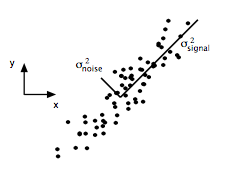
\includegraphics[width=8cm]{images/PCA_donnees.png}
	\caption[Bruit du flux de donnée $X$ et $Y$.]{Flux de données e $X$ et $Y$. On représente ici la variance du bruit ainsi que du signal. \cite{PCA}}
	\label{bruit_PCA}
\end{figure}

\paragraph{La redondance des données.} Plusieurs électrodes peuvent avoir enregistré la même information \cite{PCA}  \cite{PCA2}. On cherche donc à supprimer ses informations répétitives afin de diminuer la quantité d'informations à traiter. La mesure de la covariance représentant le degrés de relation linaire entre deux jeux de données. On recherche alors la transformation linéaire permettant de diminuer sa valeur (figure : \ref{redondance}).   

\begin{figure}[h]
	\centering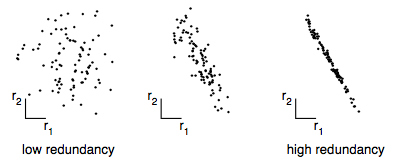
\includegraphics[width=12cm]{images/redondance.png}
	\caption[Redondances possibles dans les données dans deux flux de données R1 et R2.]{Redondances possibles des données dans deux flux de données R1 et R2. Les deux mesures à gauche ne sont pas corrélées. Les deux mesures à droite sont quant à elles fortement corrélées. \cite{PCA}}
	\label{redondance}
\end{figure}

\paragraph{La matrice de covariance.} Elle est constituée de la covariance et de la variance d'un ensemble de jeux de données \cite{PCA2}. On cherche donc à maximiser la variance (donc SNR) et à annuler les valeurs de covariances (i.e. réduire la redondance). La solution optimale revient donc à diagonaliser la matrice.

\[M =\begin{bmatrix}
\sigma^2_{x_1} & \sigma_{x_1x_2} & ... &\sigma_{x_1x_m}
\\\sigma_{x_2x_1} & \sigma^2_{x_2} & ... &\sigma_{x_2x_m} 
\\ ...&... &\sigma^2_{x_3} &...
\\ \sigma_{x_mx_1}&\sigma_{x_mx_2} & ...&\sigma^2_{x_m}  
\end{bmatrix}\]

\paragraph{Diagonalisation de la matrice de covariance.} Soit $S_X$ la matrice de covariance de $X$, on cherche à déterminer la transformation linéaire $P$, de manière à ce que $S_Y$, la matrice de covariance de $Y$, soit diagonalisée \cite{PCA}  \cite{PCA2}. 
On a donc : 
\begin{equation}
	\begin{split}
	 S_Y &= \frac{1}{n}YY^T \\
	&= \frac{1}{n}(PX)(PX)^T \\
	&= \frac{1}{n}PXX^TP^T \\
	S_Y &= PS_XP^T 
	\end{split}
\end{equation}
D'après le théorème de diagonalisation orthogonale d'une matrice symétrique (une matrice de covariance étant par définition symétrique), $S_X$ peut être exprimée par $EDE^T$, où $D$ est une matrice diagonale et $E$ est la matrice de vecteurs propres de $A$, arrangés en colonnes. On sélectionne $P$ de manière à ce que chacune de ses colonnes soit un vecteur propre de $S_X$. On pose  $P = E^T$, on a donc $ A = P^TDP$.

On obtient : 
\begin{equation}
	\begin{split}
	S_Y &= PS_xP^T \\
	& = P(E^TDE)P^T \\
	& = P(P^TDP)P^T \\
	& = (PP^T)D(PP^T) \\
	& = (PP^{-1})D(PP^{-1})\\
	S_Y& = D\\ 
	\end{split}
\end{equation}

Le choix de $P$ diagonalise bien $S_X$. Les composantes principales de $X$ sont les vecteurs propres de $S_X$.

\paragraph{Algorithme du PCA} \cite{PCA}  \cite{PCA2}:
\begin{enumerate}
	\item Soustraire la moyenne de chaque source à elle même. La moyenne des données devient alors nulle, simplifiant ainsi le calcul de la variance et de la covariance.
	\item Calculer la matrice de covariance. 
	\item Calculer les valeurs propres et vecteurs propres de la matrice de covariance. 
	\item Trier les vecteurs propres en fonction de la valeur des valeurs propres qui y sont rattachées (du plus grand au plus petit). Le vecteur des valeurs propres triées correspond au vecteur caractéristique. 
	\item Dériver les nouvelles données. On multiplie la transposée du vecteur caractéristique par les données dé-moyennées.   
\end{enumerate}

\subsubsection{Analyse en composantes indépendantes (ICA)}
\label{Subsecton : 4.ICA}
La méthode de filtrage spatiale par analyse des composantes indépendantes permet de réduire le nombre de données à traiter comme la PCA. De plus, elle permet de retrouver les signaux sources à partir des signaux enregistrés par les électrodes\cite{ICA} (Figure : \ref{conceptBSS}). 

\begin{figure}[h]
	\centering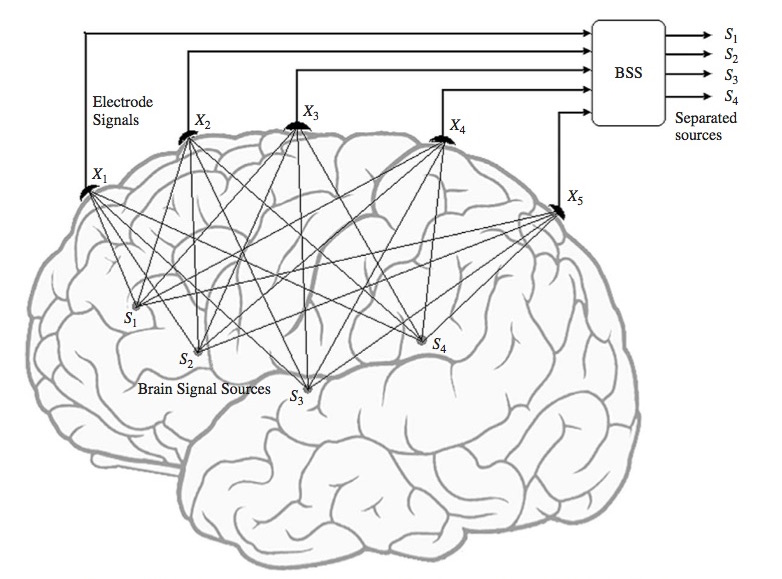
\includegraphics[width=0.6\textwidth]{images/conceptBSS.jpg}
	\caption[ICA et principe du BSS]{Principe du BSS appliqué à la détection de sources des caractéristiques du cerveau humain. $Si$ correspondent aux sources et $xi$ aux électrodes mesurant les signaux à la surface du crâne.\cite{Saeid}}
	\label{conceptBSS}
\end{figure}

Soient $S_i$ les signaux sources indépendants (l'amplitude de $S_1$ ne dépend pas de celle de $S_2$), $X_i$ les signaux enregistrés par les électrodes, $A$ la transformation linéaire mixant les sources $S_i$ en $X_i$.

\begin{equation}
X_i = AS_i
\end{equation}

 Le but est donc de retrouver la matrice $A$ et son inverse afin de reconstruire les signaux sources $S_i$ à partir de ceux observés $X_i$. Soit $S_i'$ une estimation des sources $S_i$, on doit donc déterminer la matrice $W$, elle même une approximation de $A^{-1}$

 \begin{equation}
 S_i' = WX_i
 \end{equation}

On a alors une équation à deux inconnues, ce qui est impossible à résoudre sous la forme actuelle. Une solution est d'utiliser la décomposition en valeurs singulières (SVD). 

\paragraph{La décomposition en valeurs singulières.} Une matrice est décomposable en trois opérations linéaires simples \cite{ICA}:
\smallbreak
\begin{itemize}
	\item Une rotation $V$. Il s'agit alors d'une matrice orthogonale. 
	\smallbreak
	\item Un étirement (ou compression) $\Sigma$. Il s'agit alors d'une matrice diagonale. 
	\smallbreak
	\item Une rotation $U$. Il s'agit alors d'une matrice orthogonale. 
\end{itemize}

tel que : 
\begin{equation}
	A = U\Sigma V^T
\end{equation}

Avec $A \in R^{m\times n}$, $U \in R^{m\times m}$,$\Sigma \in R^{m\times n}$,$ V \in R^{n\times n}$.

Cette transformation linéaire s'apparente à un changement de repère, ce qui n'est pas sans rappeler la méthode utilisée pour la PCA (Figure : \ref{svd}). 

\begin{figure}[h]
	\centering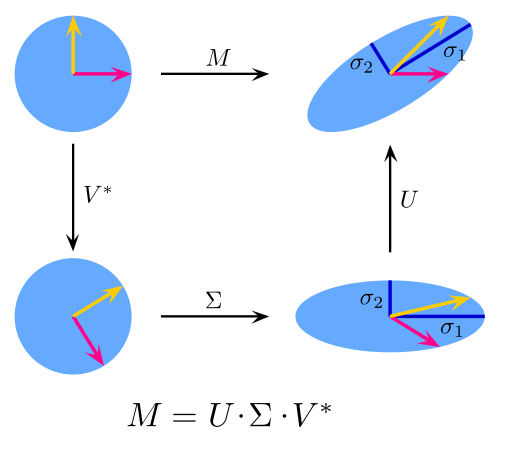
\includegraphics[width=0.6\textwidth]{images/SVD.png}
	\caption[Décomposition en valeurs singulières]{La décomposition en valeurs singulières s'apparente à décomposer une matrice en trois opérations linéaires simples : deux rotations $U$ et $V$ et un étirement $\Sigma$. $\sigma_1$ et $\sigma_2$ correspondent aux valeurs singulières. \\Source : https://fr.wikipedia.org/wiki/Décomposition\_en\_valeurs\_singulières}
	\label{svd}
\end{figure}

On peut écrire : 
\begin{equation}
	W = A^{-1} = V \Sigma^{^-1} U^T
\end{equation}

\paragraph{Étude de la covariance de $X_i$.}
On émet l'hypothèse suivante : soit $S_X$ la covariance des signaux sources, on a $S_X = I$ (une matrice de covariance étant par définition symétrique). De plus, on rappelle que pour une matrice orthogonale, $V^{-1}=V^T$. La covariance des signaux observés par les électrodes peut alors être exprimée comme suit : 
\begin{equation}
\begin{split}
S_X &= \frac{1}{n}XX^T \\
&= \frac{1}{n}(AS)(AS)^T \\
& = \frac{1}{n}(U\Sigma V^TS)(U\Sigma V^TS)^T  \\
& = U\Sigma V^T(\frac{1}{n}SS^T)V\Sigma U^T  \\
& = U\Sigma V^{-1}V\Sigma U^T \\
S_X &=  U\Sigma^2 U^T \\
\end{split}
\end{equation}

Si on pose $E = U$ avec $E$ une matrice dont les colonnes correspondent aux vecteurs propres de $S_X$, $D = \Sigma^2$ avec $D$ une matrice diagonale. On obtient alors :
\begin{equation}
	S_X = EDE^T
\end{equation}

Ce qui correspond à la propriété sur les matrices symétriques qui dit qu'une matrice peut être diagonalisée par ses vecteurs propres. 
On peut alors reformuler la valeur de $W$ : 
\begin{equation}
	W = VD^{-\frac{1}{2}}E^T
\end{equation}

Multiplier par $D^{-\frac{1}{2}}E^T$ revient jusqu'ici à réaliser une analyse en composantes principales, c'est à dire à supprimer les composantes dépendantes (redondance des informations). Soit $X_w = D^{-\frac{1}{2}}E^TX$ les données de $X$ dont les dépendances ont été supprimées et d'après l'équation 4.4, on a :
\begin{equation}
	S_i' = VX_w
\end{equation}

Il nous reste donc à caractériser la transformation linéaire $V$.
 
\paragraph{Résolution de V.} On cherche la valeur de la matrice de rotation $V$ tel que les sources $S_i'$ soient statistiquement indépendantes \cite{ICA}. i.e. 

\begin{equation}
	P(s) = \prod P(S_i)
\end{equation}

Avec P(s) la loi de probabilité de la source $S$ et $P(S_i)$ la loi de probabilité de l'ensemble des sources $S_i$.
La mesure des statistiques indépendantes entre plusieurs variables peut être déterminée par l'équation de multi-information suivante :

\begin{equation}
	I(S) = \int{P(S)log_2 \frac{P(S)}{\prod_iP(S_i)}dy}
\end{equation}

Si $I(S) = 0$, cela signifie que les sources sont totalement indépendantes. En effet, si $P(S) = \prod_i P(S_i)$, on a $log(\frac{P(S)}{\prod_iP(S_i)}) = log(1) = 0$. Il faut donc trouver la matrice $V$ tel que $I(S) = 0$.

\paragraph{Algorithme de l'ICA} \cite{ICA}
\smallbreak
\begin{enumerate}
	\item Soustraire la moyenne de chaque source à elle même. La moyenne des données devient alors nulle, simplifiant ainsi le calcul de la variance et de la covariance.
	\item Calculer la matrice de covariance. 
	\item Calculer les valeurs propres $D$ et vecteurs propres $E$ de la matrice de covariance.
	\item Dériver les nouvelles données. On multiplie la transposée du vecteur caractéristique par les données dé-moyennées. Le résultat correspond aux signaux observés sur les électrodes, dont on a supprimé les dépendances. Soit $E^TX$.
	\item Multiplier le résultat précédent par la racine du vecteur des valeurs propres. soit $X_w = D^{-\frac{1}{2}}E^TX$.
	\item Calculer la rotation ($V$) qui maximise la corrélation des données. 
	\item Calculer $W = VD^{-\frac{1}{2}}E^T$.
	\item On peut alors retrouver les signaux sources $S_i$ en calculant $S_i = W \times X_0$.
\end{enumerate}

Les étapes 1 à 4 correspondent à une analyse en composantes principales.

\subsubsection{Configuration Spatiale Commune (CSP)}
\label{Subsubsecton : 4.CSP}
La méthode CSP est utilisée à la fois en filtrage spatial et pour les algorithmes de sélection automatique de canaux (signaux de sortie des électrodes) \cite{CSP} \cite{Lotte}. Tout comme l'algorithme du PCA, on cherche ici à réaliser une transformation linéaire sur un flot de données, afin de décorréler les sources entres elles. À la différence qu'ici, on a en entrée du filtre deux jeux de données, que l'on appellera des classes. Dans notre cas, il peut s'agir d'une classe "stimulus gauche" correspondant aux signaux générés après le mouvement de la main gauche, ou d'une classe "stimulus droit" correspondant aux signaux générés après le mouvement de la main droite. On cherche alors à maximiser la variance et à minimiser la covariance entre les deux classes. On a donc deux étapes principales : 
\smallbreak
\begin{enumerate}
	\item Maximiser la variance et minimiser la covariance des sources de chacune des classes. 
	\smallbreak
	\item Maximiser la variance de chacune des deux classes et minimiser la covariance entre les deux classes.  
\end{enumerate}

Soit $R_H$ et $R_F$ les covariances des classes $H$ et $F$, tels que :

\begin{equation}
	R_H = \frac{X_H X^T_H}{Trace(X_H X^T_H)} \ \ R_F = \frac{X_F X^T_F}{Trace(X_F X^T_F)}
\end{equation}

Avec $X_H$ et $X_F$ les données de la classe $H$ et $X_F$ les données de la classe $F$. 
La covariance spatiale totale correspond à la somme des covariances des deux classes : 

\begin{equation}
	R = R_H + R_F 
\end{equation}

\paragraph{Algorithme du CSP}
\begin{enumerate}
	\item Soit $X_g$ un ensemble de sources de données EEG  correspondant aux réponses cérébrales lors du mouvement de la main gauche et $X_d$ un ensemble de données correspondant aux réponses cérébrales lors du mouvement de la main droite. On soustrait la moyenne de chacune des sources des deux ensembles à elles-mêmes. La moyenne des données devient alors nulle, simplifiant ainsi le calcul de la variance et de la covariance.
	\item Calculer la matrice de covariance des deux ensembles $X_g$ et $X_d$. On appellera $R_g$ la matrice de covariance de l'ensemble $X_g$ et $R_d$ la matrice de covariance de l'ensemble $X_d$.
	\item Calculer les valeurs propres $D$ et vecteurs propres $E$ de la matrice de $R_g$ et $R_d$.
	\item Dériver les nouvelles données. On multiplie la transposée du vecteur caractéristique par les données dé-moyennées. Le résultat correspond aux signaux observés sur les électrodes, dont on a supprimé les dépendances, soit $E^TX$.
	\item Multiplier le résultat précédent par la racine du vecteur des valeurs propres. soit $X_w = D^{-\frac{1}{2}}E^TX$.
	\item Calculer la valeur des sources des deux ensembles, soit $S_g = WR_gW^T$ et $S_d = WR_dW^T$.
	\item Calculer la rotation ($V$) qui maximise la corrélation des données. 
	\item Calculer $W = VD^{-\frac{1}{2}}E^T$.
	\item Calculer les valeurs propres $D$ et vecteurs propres généralisés $B$ des sources $S_g$ et $S_d$.
	\item Trier les vecteurs propres en fonction de la valeur des valeurs propres qui y sont rattachées (du plus grand au plus petit).
	\item Le calcul du poids à attribuer à chacun des canaux est déterminé de la manière suivante : $Poids = B'W$
\end{enumerate}


\subsection{Méthodes d'extraction des caractéristiques}
\label{Subsecton : 4.Méthodes d'extraction des caractéristiques}

\subsubsection{Filtrage temporel}
\label{Subsub : 4.Méthodes d'extraction des caractéristiques}
La phase d'extraction des données consiste dans un premier temps à réaliser un filtrage temporel afin d'extraire du signal EEG les rythmes du cerveau (caractéristiques) qui nous intéressent. Pour cela, on réalise un filtrage passe-bande. Les deux types de filtres les plus utilisés en traitement du signal sont les filtres de Butterworth et Chebychev. 

\begin{itemize}
	\item \textbf{Filtre de Butterworth.} Il s'agit d'un filtre qui possède un gain quasiment constant dans sa bande-passante (on parle de critère de méplat). L'avantage est qu'il engendre très peu de distorsions dans la bande passante. Sa réponse en phase est presque linéaire. Cependant sa réjection est moins importante dans la bande coupante, dû à la "limitation" de la bande de coupure.
	\smallbreak
	\item \textbf{Filtre de Chebychev.} Il s'agit d'un filtre dans lequel on introduit une oscillation (distorsion contrôlée), permettant d'obtenir une "vitesse" de coupure plus importante. L'inconvénient de ce filtre est que les oscillations introduites entrainent des distorsions de phase sur le signal de sortie. 
	\smallbreak
\end{itemize}

Il est préférable d'utiliser une filtre de type Butterworth dans notre cas car on ne peut pas tolérer l'introduction de distorsions dans les rythmes du cerveau. On propose donc d'utiliser un filtre passe-bande d'ordre 5.

\subsubsection{Représentation spectrale}

Une fois les caractéristiques extraites, on souhaite les représenter dans le domaine spectral afin de structurer les données pour la classification. La méthode majoritairement utilisée dans le traitement des signaux EEG est la transformée de Fourier à court terme (TFCT). Il s'agit d'une méthode dérivée de la transformée de Fourier rapide (FFT) qui gère la non-stationnarité des signaux d'entrée en les fenêtrant. Concrètement, cela revient à calculer la FFT, puis à appliquer un fenêtrage \cite{feature}.
 
 \begin{center}
 $
 STFT(x(t)) = X(\tau,u) = \int_{-\infty}^{\infty}x(t)w(t-\tau)e^{-j2\pi.ut}dt
 $
\end{center}

Avec $X(t,\tau)$ la transformée de $x(t)w(t-\tau)$, $x(t)$ le signal à transformer, $w(t)$ le signal de fenêtrage, $\tau$ la valeur de décalage temporel des fenêtres et $u$ la fréquence. Il s'agit la plupart du temps d'un fenêtrage de pondération de Hanning ou de Gauss, qui offre à la fois une bonne résolution spectrale et une bonne dynamique au filtrage. 
Si on discrétise les valeurs, on obtient le calcul de la STFT suivant : 

 \begin{center}
$
 STFT(x[n])=\sum_{0}^{N-1}x(n)w(n-m)e^{-j2.\pi\frac{nk}{N}}
 $
 \end{center}
 
 avec $k$ l'échantillon calculé, $N$ le nombre de points et $n$ la variable.
 
 La largeur des fenêtres étant constante, on observe une diminution de la résolution temporelle lorsque les fréquences deviennent trop faibles.

\begin{figure}[h]
	\centering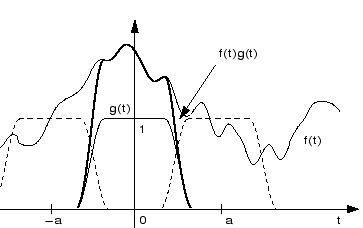
\includegraphics[width=9cm]{images/STFT.png}
	\caption[STFT du signal f(t), avec fenêtrage par le signal g(t)]{STFT du signal f(t), avec fenêtrage par le signal g(t)\\https://www.math.ucdavis.edu/~strohmer/research/gabor/gaborintro/img47.gif}
	\label{stft}
\end{figure}

\subsection{Méthodes de classification}
\label{subsection : 4.Méthodes de classification}
La phase de classification consiste à trier et à classifier des échantillons dans une catégorie (classe). 

Dans le cas général, les données d'entrées sont les suivantes :
\smallbreak
\begin{itemize}
	\item P classes d'objets du même type.
	\smallbreak
	\item N observables définies pour toutes les classes.
	\smallbreak
	\item Pour chacun des P classes, un échantillon d'objets Nk  (k étant l'indice de classe).
	\smallbreak
\end{itemize}

Pour classifier un nouvel objet dans une des classes définies, on passe par cinq phases distinctes :
\smallbreak
\begin{itemize}
	\item La collecte des données.
	\smallbreak
	\item La caractérisation des classes.
	\smallbreak
	\item Le choix d'un algorithme de classification.
	\smallbreak
	\item L'apprentissage.
	\smallbreak
	\item Les tests.
	\smallbreak
\end{itemize}

Nous avons étudié les 3 algorithmes de classification suivants et nous les avons comparé en fonction leurs applications possibles, leurs avantages et leurs inconvénients \cite{Faivre}.

\subsubsection{Linear Discriminant Analysis}
\label{Subsubsection : 4.Linear Discriminant Analysis}
L'analyse discriminante linéaire (LDA) est l'algorithme le plus populaire dans le domaine des interfaces cerveau-ordinateur (BCI).

Il est réputé comme étant un classificateur stable en raison de sa faible complexité, il s'appuie sur des calculs simples, et est adapté à la classification en temps réel (Figure \ref*{classiLDA}).
 
\begin{figure}[h]
	\centering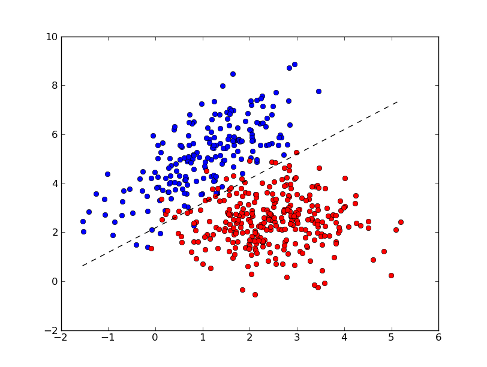
\includegraphics[width=8cm]{images/lda.png}
	\caption{Classification LDA}
	\label{classiLDA}
\end{figure}

\smallbreak
\textbf{Principes de LDA : }
\smallbreak

Le principe de la méthode LDA est illustré par les deux figures suivantes. Il a été supposé que deux observables , X et Y, étaient accessibles à l'observateur. Les zones bleues sont éliminées par les coupures (qui sont représentées par les lignes bleues).

Les deux premiers graphiques montrent le résultat de coupes classiques : on peut voir le compromis réalisé dans les deux cas entre précision et efficacité (Figure \ref{principeLDA1}).


\begin{figure}[h]
	\centering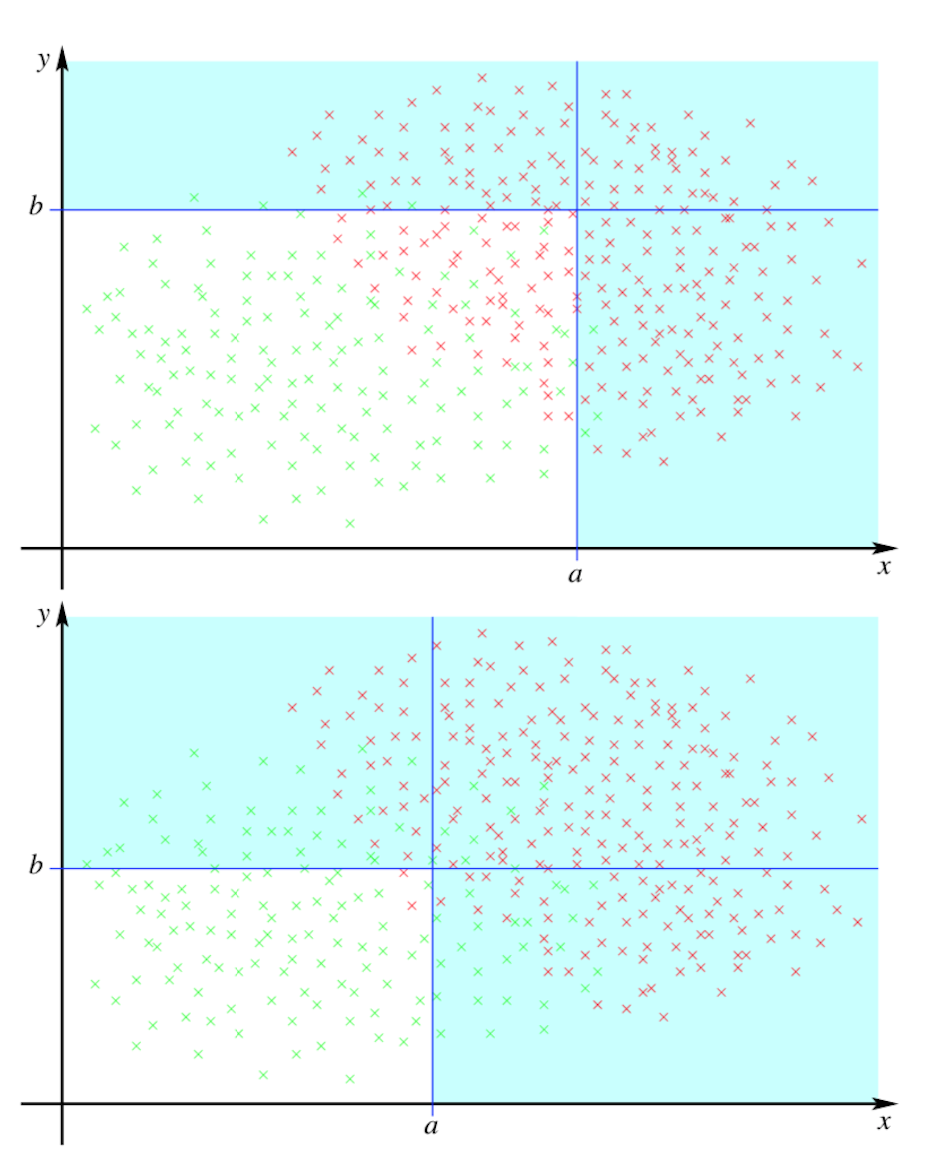
\includegraphics[width=8cm]{images/principeLDA1.png}
	\caption[Principe de LDA 1]{Principe de LDA 1 \cite{Faivre}}
	\label{principeLDA1}
\end{figure}

LDA consiste à découper le long d'une combinaison linéaire de tous les observables, plutôt que le long de chacun des observables. Cette combinaison linéaire est définie par une direction LDA (ou axe). 

L'algorithme consiste à calculer la direction de cet axe de manière à avoir une discrimination optimale entre les classes conformément à un critère donné. Un hyperplan perpendiculaire à l'axe est alors associé à cette discrimination (Figure \ref{principeLDA2}]).

\begin{figure}[h]
	\centering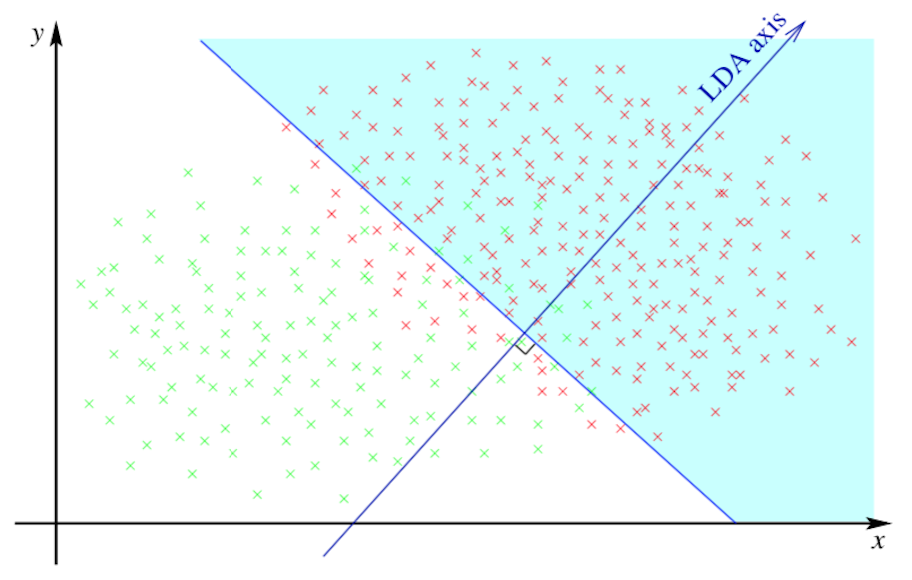
\includegraphics[width=8cm]{images/principeLDA2.png}
	\caption[Principe de LDA 2]{Principe de LDA 2 \cite{Faivre}}
	\label{principeLDA2}
\end{figure}

\textbf{Hypothèses et formules : }
\smallbreak

L’objectif est de produire une règle d’affectation $X(\omega) \mapsto Y(\omega)$ qui permet de prédire, pour une observation $\omega$ donnée, sa valeur associée de Y à partir des valeurs prises par X.

La règle bayesienne consiste à produire une estimation de la probabilité à posteriori (appuyée sur les expériences et les faits) d’affectation :

\begin{equation}
P(Y=y_k ~|~ X) = \frac{P(Y=y_k) \times P(X ~|~ Y=y_k)}{\sum_{i=1}^K P(Y=y_i) \times P(X ~|~ Y=y_i)}
\end{equation}

$P(Y=y_k)$ est la probabilité d’appartenance à une classe. $P(X ~|~ Y=y_k)$ représente la fonction de densité des X conditionnellement à la classe $y_k$.

La règle d’affectation pour un individu $\omega$ à classer devient alors :

\begin{equation}
Y(\omega) = \arg\max_{k}\ P(Y=y_k ~|~ X(\omega))
\end{equation}

Toute la problématique de l’analyse discriminante revient alors à proposer une estimation de la quantité :

\begin{equation}
P(X ~|~ Y = y_k)
\end{equation}

On distingue principalement deux approches pour estimer correctement la distribution $P(X ~|~ Y=y_k)$ :
\smallbreak
\begin{itemize}
	\item L’approche non-paramétrique n’effectue aucune hypothèse sur cette distribution mais propose une procédure d’estimation locale des probabilités, au voisinage de l’observation $\omega$, à classer. Les procédures les plus connues sont la méthode d'estimation par noyau et la méthode des plus proches voisins.
	\smallbreak
	\item La seconde approche effectue une hypothèse sur la distribution des nuages de points conditionnels, on parle dans ce cas d’analyse discriminante paramétrique. Exemple : hypothèse de multinormalité, etc.
	\smallbreak
\end{itemize}

\subsubsection{Support Vector Machine}
\label{subsubsection : 4.Support Vector Machine}
SVM est une méthode de classification binaire par apprentissage supervisé, destinée à résoudre des problèmes de discrimination (décider à quelle classe appartient un échantillon) et de régression (prédire la valeur numérique d'une variable). 

Cette méthode repose sur l'existence d’un classificateur linéaire dans un espace approprié. 

Puisque c’est un problème de classification à deux classes, cette méthode fait appel à un jeu de données d'apprentissage pour apprendre les paramètres du modèle. Elle est basée sur l'utilisation de fonction dites noyau qui permettent une séparation optimale des données. 

Après la méthode  LDA, c'est la deuxième méthode la plus populaire parmi les classificateurs linéaires.

\subsubsection{Bayes quadratique}
\label{subsubsection : 4.Bayes Quadratique}
Cette approche est basée sur le calcul de la probabilité de chaque classe, compte tenu du vecteur de caractéristiques. Bayes quadratique assigne le signal EEG à la classe la plus probable. Ce classificateur nest pas très populaire pour les systèmes BCI, cependant , il reste assez précis pour la classification de l'imagerie motrice (motor imagery) comparé à d'autres méthodes.

Nous avons décidé de partir sur l'algorithme LDA car nous souhaitons travailler en temps réel, et il se trouve que la méthode LDA  semble être la plus performante pour ce genre de tâche.


%Bibliographie : 

% Site web de McGill : http://lecerveau.mcgill.ca/flash/i/i_01/i_01_cr/i_01_cr_ana/i_01_cr_ana.html#2    

% Livre EEG Signal Processing 

% Mémoire de Olivier St-Amand " Techniques de traitement de signal appliquées aux essais individuels évoqués

%SSVEP A Survey of Stimulation Methods Used in SSVEP-Based BCIs
  \chapter{Utilisation du casque EPOC et d'OpenViBE}
\label{Chapitre : Utilisation du casque EPOC et d'OpenViBE}
\thispagestyle{fancy}

\section{OpenViBE}
\label{Section : 5.OpenViBE}

\subsection{Généralités sur le fonctionnement d'OpenViBE}
\label{Subsection : 5.Généralités sur le fonctionnement d'OpenViBE}
OpenViBE est une plateforme logicielle dédiée à la conception et à l'utilisation d'interfaces cerveau-ordinateur en temps réel. Celle-ci est éditée par l'Institut National de Recherche en Informatique et en Automatique (INRIA) de Rennes en France. Le logiciel gère à la fois l'acquisition, le traitement et l'analyse des signaux.

OpenViBE fonctionne sous forme de scénarios, correspondant à un ensemble de blocs fonctionnels. La suite OpenViBE est composée de deux logiciels : 
\smallbreak
\begin{itemize}
	\item \textbf{OpenViBE designer}. Il s'agit d'un éditeur de scénario permettant de  créer et modifier les schémas blocs grâce à une interface graphique. Il suffit alors de placer les différents blocs désirés, de les configurer (en cliquant dessus), et de les relier pour former une chaine de traitement (procédure).
	\smallbreak
	\item \textbf{OpenViBE acquisition server.} Permet d'acquérir des données EEG brutes à partir d'un dispositif EEG. Il est par exemple possible de connecter différents types de casques comme le casque EPOC d'Emotiv.
	\smallbreak
\end{itemize}

Il est possible d'envoyer des données d'OpenVIBE vers une application externe via une connexion VRPN (Virtual Reality Peripheral Network).

\subsection{Installation d'OpenViBE}
\label{Subsection : 5.Installation d'OpenViBE}
 Le logiciel fonctionne sous les systèmes d'exploitations Windows (Windows XP ou ultérieur, la stabilité du logiciel sous Windows 8 n'ayant pas été vérifiée par l'éditeur) et Linux (Ubuntu, Fedora). La liste détaillée des architectures compatibles avec OpenViBE est disponible à l'adresse suivante : http://openvibe.inria.fr/supported-architectures/.
Il est possible de télécharger l'installeur OpenViBE à l'adresse suivante : http://openvibe.inria.fr/downloads/. Une fois celui-ci téléchargé, il suffit de l'ouvrir et de suivre les indications affichées à l'écran.

\subsection{Utilisation d'OpenViBE designer}
\label{Subsection :5.Utilisation d'OpenViBE designer}

\subsubsection{Description de l'interface de contrôle de la simulation}
\label{Subsubsection : 5.Description de l'interface de contrôle de la simulation}
La partie supérieure de l'interface graphique permet de contrôler la simulation, i.e. le déroulement du scénario. Ainsi, il est possible de lancer un scénario en appuyant sur le bouton "lecture", de le stopper en appuyant sur le bouton "stop", d'en accélérer le déroulement en appuyant sur le bouton "avance rapide", etc. Il est également possible de lancer plusieurs scénarios en même temps (Figure : \ref{fig:interface_simu_ov}). 

\begin{figure}[h]
	\centering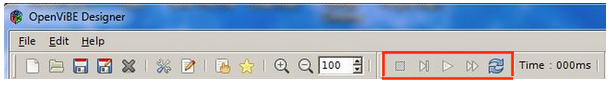
\includegraphics[height=2cm]{images/interface_simu_ov.png}
	\caption{Interface de contrôle de la simulation sous OpenViBE.}
	\label{fig:interface_simu_ov}
\end{figure}

\subsubsection{Description de l'interface du répertoire des blocs fonctionnels}
\label{Subsubsection : 5.Description de l'interface du répertoire de blocs fonctionnels}
La partie située à droite de l'interface graphique de l'éditeur permet de rechercher les blocs désirés afin de construire un scénario. Ceux-ci sont triés en différentes catégories. un simple glisser-déposer permet de placer un bloc dans l'espace de travail (Figure : \ref{fig:interface_bloc_ov}).

\begin{figure}[h]
	\centering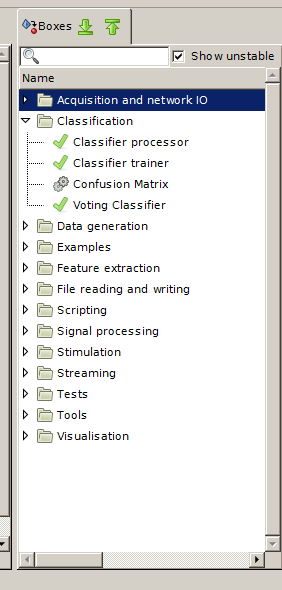
\includegraphics[height=7cm]{images/interface_bloc_ov.png}
	\caption{Interface du répertoire des blocs OpenViBE.}
	\label{fig:interface_bloc_ov}
\end{figure}

\subsubsection{Description de l'espace de travail}
\label{Subsubsection : 5.Description de l'espace de travail}
La partie centrale de l'interface graphique correspond à l'espace de travail d'OpenViBE. C'est ici où l'on construit les différents scénarios de l'interface cerveau-ordinateur, via des blocs fonctionnels. Chaque bloc peut être relié à un autre en maintenant la souris sur la sortie d'un bloc, vers l'entrée d'un autre bloc. On peut seulement connecter une entrée à une sortie du même type (e.g. une entrée de type "signal" vers une sortie de type "signal") (Figure : \ref{fig:interface_travail_ov}).

\begin{figure}[h]
	\centering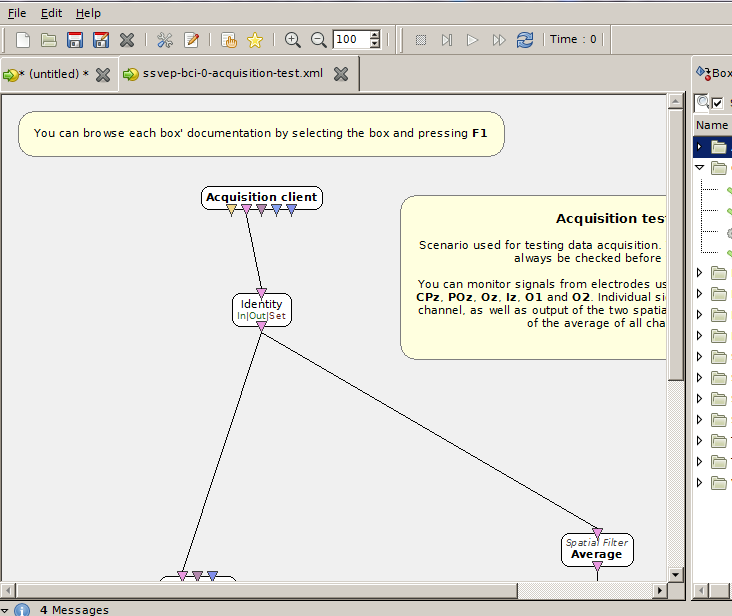
\includegraphics[height=8cm]{images/interface_travail_ov.png}
	\caption{Espace de travail d'OpenViBE.}
	\label{fig:interface_travail_ov}
\end{figure}

\subsection{Description des blocs utilisés}
\label{Subsection : 5.Description des blocs utilisés}
Voici la liste des différents blocs utilisés dans le cadre de notre projet :

\subsubsection{Acquisition et Réseau}
\label{Subsubsection : 5.Acquisition et Réseau}
\begin{itemize}
	\smallbreak
	\item \textbf{Acquisition Client.} Ouvre une interface de connexion pour lire les information envoyées par le serveur d'acquisition (i.e. les données du casque en temps réel). Il faut pour cela indiquer le port utilisé par le serveur (1024 par défaut).
	\smallbreak
	\item \textbf{Analog VRPN Server.} Permet d'envoyer des données à une application client via le protocole VRPN.
\end{itemize}
\subsubsection{Traitement de signal}
\label{Subsubsection : 5.Traitement de signal}
\begin{itemize}
	\smallbreak
	\item \textbf{Temporal Filter}. Réalise le filtrage temporel d'un signal. Il est possible de choisir la méthode de filtrage (passe-bas, passe-bande ou passe-haut), le type (Butterworth, Chebychev) et l'ordre de filtre.
	\smallbreak
	\item \textbf{Spatial Filter}. Permet de réaliser un filtrage spatiale statique, i.e. en paramétrant le poids attribué à chaque canal d'entrée manuellement. (filtrage bipolaire, Laplacien, etc.)
	\smallbreak
	\item \textbf{FastICA.} Permet de réaliser un filtrage spatial via l'algorithme ICA (\ref{Subsecton : 4.ICA}). Attention, le bloc est cependant considéré comme non stable par l'INRIA.
	\smallbreak
	\item \textbf{CSP Spatial Filter Trainer.} Permet réaliser un filtrage spatial via l'algorithme CSP (\ref{Subsubsecton : 4.CSP}).
	\smallbreak
	\item  \textbf{Time Based Epoching.} Permet de découper un signal en plusieurs morceaux ayant une durée et un intervalle spécifié.
	\smallbreak
	\item \textbf{Simple DSP.} Permet de réaliser des algorithmes mathématiques simples.
	\smallbreak
	\item \textbf{Signal Average.} Permet de calculer la moyenne d'un signal.
	\smallbreak
	\item \textbf{Spectral Analysis (FFT).} Réalise l'analyse spectrale de signaux en utilisant la FFT (Fast Fourier Transform).
	\smallbreak
	\item \textbf{ Spectrum Average.} Calcule la moyenne de toutes les puissances de bande de fréquence pour un spectre donné.
\end{itemize}
\subsubsection{Classification}
\label{Subsubsection : 5.Classification}
\begin{itemize}
	\smallbreak
	\item \textbf{Classifier Trainer.} Permet de réaliser des algorithmes de classification. Ce bloc effectue plus particulièrement l'entrainement du classificateur. Les différents algorithmes proposés sont la LDA et la SVM.
	\smallbreak
	\item \textbf{Classifier Processor.} Permet de réaliser la classification de vecteurs  caractéristiques entrants, en utilisant un classificateur entrainé précédemment.
	
\end{itemize}
\subsubsection{Lecture et écriture de fichiers}
\label{Subsubsection : 5.Lecture et écriture de fichiers}
\begin{itemize}
	\smallbreak
	\item \textbf{Generic Stream Writer.} Permet d'écrire des données dans un fichier binaire. Extension du fichier : .ov
	\smallbreak
	\item \textbf{Generic Stream Reader.} Permet de lire un fichier enregistré grâce à un bloc Generic File Writer.
	\item \textbf{CSV File Reader.} Ce bloc permet de lire des données (signaux par exemple) issues d'un fichier CSV (Comma-Separated Values). Le format  CSV est ouvert et représente les données sous la forme de valeurs séparées par des virgules (format Européen), des points-virgules (format Américain) ou des tabulations. Ce bloc peut-être utilisé pour réaliser l'importation de données depuis Matlab ou Octave. 
	\smallbreak
	\item \textbf{CSV File Writer.} Ce bloc permet d'écrire des données issues d'OpenViBE dans un fichier CSV. Il peut par exemple être utilisé pour réaliser de l'exportation de données vers Matlab ou Octave.
\end{itemize}
\subsubsection{Simulation}
\label{Subsubsection : 5.Simulation}
\begin{itemize}
	\smallbreak
	\item\textbf{Player Controller.} Permet de contrôler l'arrêt et la mise en pause d'un scénario à l'aide des stimulations reçues. 
\end{itemize}
\subsubsection{Visualisation}
\label{Subsubsection : 5.Visualisation}
\begin{itemize}
	\smallbreak
	\item\textbf{Signal Display.} Permet d'afficher un signal en temps réel.
	\smallbreak
	\item\textbf{Power Spectrum Display.} Permet d'afficher l'amplitude d'un signal dans un ensemble de bandes de fréquences.
	\smallbreak
	\item \textbf{2D Topographic Map.} Permet d'afficher la topographie de l'activité cérébrale en 2 dimensions.
	\smallbreak
	\item \textbf{3D Topographic Map.} Permet d'afficher la topographie de l'activité cérébrale en 3 dimensions.
	\smallbreak
	\item\textbf{Graz Visualisation.} Permet d'afficher la consigne et le résultat en temps réel.
\end{itemize}
\subsubsection{Autres}
\label{Subsubsection : 5.Autres}
\begin{itemize}
	\smallbreak
	\item \textbf{Feature aggregator.} Permet de rassembler les différentes entrées du bloc vers un vecteur caractéristique.
	\smallbreak
	\item\textbf{Identity }. Duplique l'entrée de ce bloc vers sa sortie.
\end{itemize}


\subsection {Utilisation du serveur d'acquisition d'OpenViBE}
\label{Subsection : 5.Utilisation de OpenViBE acquisition Server}
On s'appuie ici sur l'utilisation d'OpenViBE acquision server afin d'acquérir les données EEG brutes à partir du casque EPOC (composé, pour rappel, de 14 canaux EEG). Afin d'accéder à ces données, il est nécessaire d'être en possession du SDK de ce casque (édition de recherche). De plus, il est nécessaire d'utiliser le système d'exploitation Windows afin d'assurer la compatibilité d'OpenVIBE avec le casque EPOC.

Au lancement du serveur d'acquisition d'OpenViBE, la fenêtre de configuration apparait (Figure \ref{fig:acquisition}, fenêtre de gauche).
\smallbreak
\begin{itemize}
	\item \textbf{Driver}. Indiquer le pilote correspondant au casque utilisé via le menu déroulant. Il s'agit dans notre cas du casque EPOC d'Emotiv.
	\smallbreak
	\item \textbf{Connection Port}. Permet de renseigner le port de connexion du casque. Laisser la valeur à 1024.
	\smallbreak
	\item \textbf{Sample count per sent block}. Permet de configurer la taille des paquets envoyés du casque vers OpenViBE. Laisser à 32.
	\smallbreak
\end{itemize} 

Appuyer sur le bouton "Driver properties" ouvre la fenêtre de configuration du casque (Figure \ref{fig:acquisition}, fenêtre de droite). Il faut alors renseigner les champs suivants :
\smallbreak
\begin{itemize}
	\item \textbf{Identifier}. Permet d'enregistrer les données de plusieurs utilisateurs. Laisser la valeur à 0.
	\smallbreak
	\item \textbf{Age}. Renseigner l'âge de l'utilisateur.
	\smallbreak
	\item \textbf{Gender}. Renseigner le sexe de l'utilisateur.
	\smallbreak
\end{itemize}


\begin{figure}[h]
	\centering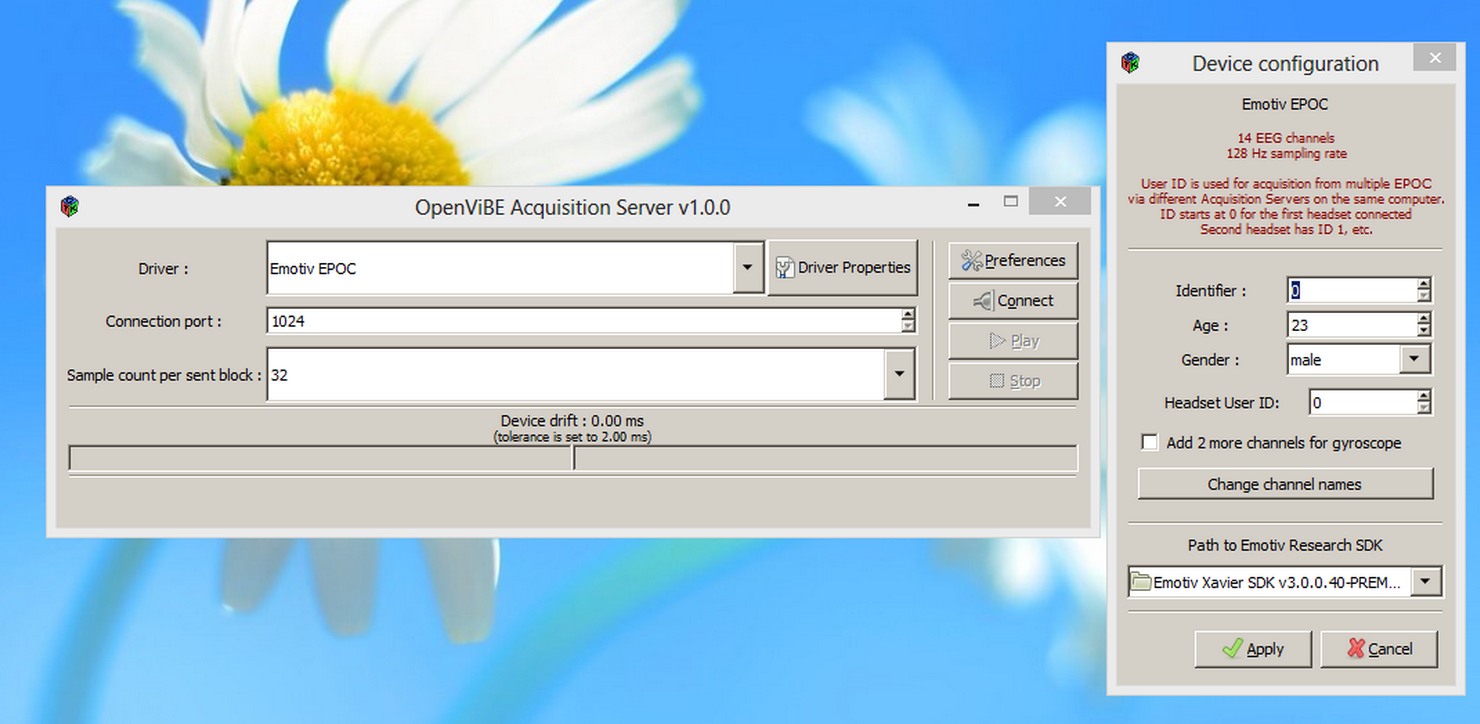
\includegraphics[height=6.5cm]{images/configOpenvibeEpoc.png}
	\caption{Lancement du serveur d'acquisition}
	\label{fig:acquisition}
\end{figure}

Ensuite, il ne reste plus qu'à appuyer sur "Connect" et sur "Play". La connexion entre le casque et OpenViBE s'effectue alors via le serveur d'acquisition. Le message "Connection succeded" informe l'utilisateur que la connexion avec le casque a été réalisée (Figure \ref{serveurUp}).

\begin{figure}[h]
	\centering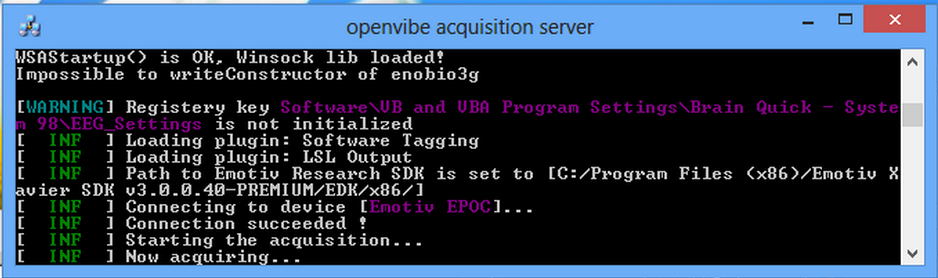
\includegraphics[height=3.5cm]{images/serveurUp.png}
	\caption{Serveur démarré}
	\label{serveurUp}
\end{figure}

\section {Utilisation du casque EPOC}
\label{Section : 5.Utilisation du casque EPOC}

\subsection{Généralités sur le fonctionnement du casque}
\label{Subsection : 5.Généralités sur le fonctionnement du casque}
Afin d'utiliser le casque EPOC d'Emotiv et d'acquérir les données EEG, il est nécessaire d'utiliser deux éléments :
\smallbreak
\begin{itemize}
	\item \textbf{Emotiv Xavier Control Panel Premium.} Il s'agit du panneau de configuration du casque EPOC. Il permet de le configurer et de le tester via une interface graphique.
	\smallbreak
	\item \textbf{ SDK Emotiv.} Il s'agit du kit de développement du casque. Dans le cadre de notre projet, il nous permettra d'utiliser le casque avec OpenViBE et d'acquérir les signaux EEG.
\end{itemize}
	
\subsection {Installation de Emotiv Xavier Control Panel Premium et du SDK.}
\label{Subsection : 5.Installation de Emotiv Xavier Control Panel Premier et du SDK}
Pour installer les deux utilitaires, il faut suivre la démarche suivante : 
\smallbreak
\begin{enumerate}
	\item Se connecter sur son compte Emotiv (https://emotiv.com/).
	\item Aller dans l'onglet "my downloads".
	\item Télécharger le SDK du casque.
	\item Une fois l'installeur téléchargé, l'ouvrir et suivre les instructions affichées à l'écran. Il vous sera demandé de fournir le code de la licence. Celui-ci est indiqué sur la page de téléchargement. L'installation de l'Emotiv Xavier Control Panel Premium s'effectuera lors de l'installation du SDK.
\end{enumerate}

\subsection {Préparation du casque}
\label{Subsection : 5.Préparation du casque}
Voici les étapes de préparation du casque : 
\smallbreak
\begin{enumerate}
	\item Bien humidifier chaque électrode avec la solution saline (jusqu’à saturation).
	\item Insérer ces électrodes sur le casque (il faut sentir un cran).
	\item Brancher la clé USB pour assurer la connexion sans fil avec le casque.
	\item Allumer le casque.
\end{enumerate}

\subsection {Conseils sur l'utilisation du casque}
\label{Subsection : 5.Conseils sur l'utilisation du casque}
\begin{itemize}
	\item Ré-hydrater les électrodes toutes les heures pour garantir un bon contact dermal et donc un signal optimal.
	\smallbreak
	\item S’assurer du bon fonctionnement du casque en vérifiant régulièrement la qualité du signal via le logiciel "Emotiv Xavier Control Panel Premium".
	\smallbreak
	\item Ranger les électrodes dans leur boite lorsque le casque n’est pas utilisé et s’assurer que le tampon soit humide (dans le cas contraire, l’humidifier avec la solution saline).
	\smallbreak
	\item Utiliser un tampon alcoolisé pour désinfecter les électrodes lorsque le casque n'est plus utilisé.
	\smallbreak
	\item Ne pas utiliser le casque lorsque sa batterie est en rechargement.
\end{itemize}

\subsection {Vérification de la qualité des signaux}
\label{Subsection : 5.Vérification de la qualité des signaux}
Afin d'exploiter de manière optimale les données provenant du casque, il est nécessaire de vérifier la qualité du signal à partir du panneau de configuration du casque. Lors de l'ouverture logiciel, et après connexion, le menu principal apparait. Sur l'interface, les différentes électrodes sont représentées par des points. Un points vert représente un signal de bonne qualité, un point orange de moyenne qualité et un point rouge ou noir correspond à un signal de mauvaise qualité (Figure \ref{qualiteSignal}).
	
\begin{figure}[h]
	\centering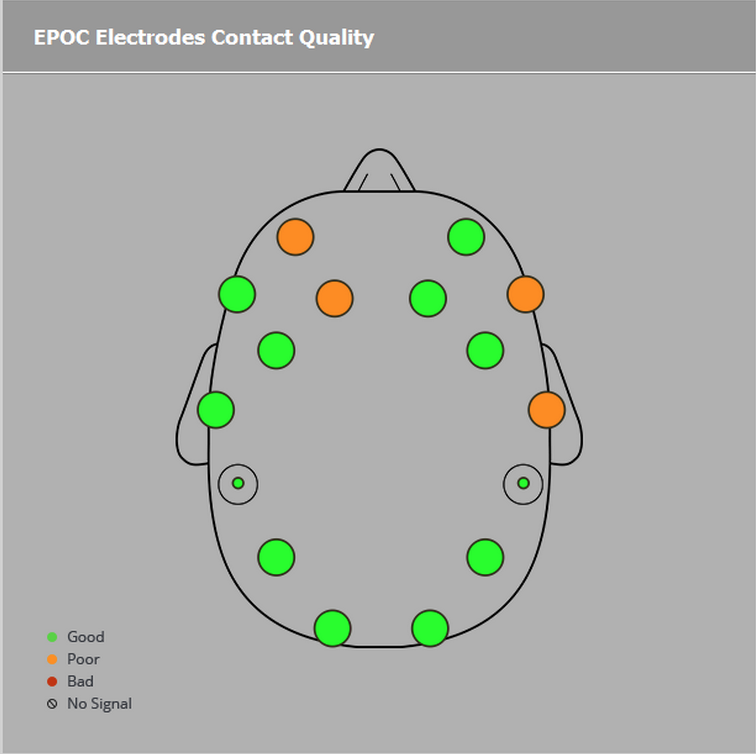
\includegraphics[height=6.5cm]{images/emotivQuality.png}
	\caption{Qualité du signal provenant des électrodes}
	\label{qualiteSignal}
\end{figure}
	
  \chapter{Expérience simple d'interaction}
\label{Chapitre : Première exprérience simple d'interaction}
\thispagestyle{fancy}

\section {Présentation de l'expérience}
\label{Section : 6.présentation de l'expérience}
Cette expérience simple d'interaction permet de mettre en application les différents aspects théoriques étudiés dans la partie 4. Celle-ci s'appuie sur la méthode d'imagerie motrice qui consiste à imaginer le mouvement de différentes parties du corps, ce qui résulte en l'activation du cortex sensorimoteur modulant les rythmes alpha et bêta du cerveau. Ces variations peuvent être détectées par l'interface cerveau-ordinateur. Il est alors possible d'en déduire les intentions de l'utilisateur.
Le but de l'expérience présentée est de déterminer si l'utilisateur pense à un mouvement de sa main droite ou de sa main gauche.
Pour cela, on se base sur l'utilisation du casque EPOC (partie \ref{Section:3.Choix du matériel}). On réalise la chaîne de traitement et d'analyse des signaux sous la forme de 5 scénarios OpenViBE (partie \ref{Section:3.Choix du logiciel} et \ref{Section : 5.OpenViBE}).





\section {Développement des scénarios sous OpenViBE}
\label{Section : 6.Développement des scénarios sous OpenViBE}



\subsection{Scénario 1 : Acquisition des données pour apprentissage}
\label{Subsection : 6.Scénario 1}

Ce scénario permet de réaliser l'acquisition des signaux EEG afin d'effectuer la configuration et l'apprentissage des filtres spatiaux et des classificateurs. Pour cela, on présente à l'utilisateur un certain nombre de stimuli visuels de façon à lui indiquer quelle est la tâche mentale à réaliser (Figure \ref{scena1}). On lui présentera par exemple 20 flèches à gauche, indiquant à celui-ci de penser à un mouvement de la main gauche et 20 flèches à droite pour imaginer un mouvement de la main droite dans un ordre aléatoire (Figure \ref{acqui}). De cette manière, OpenViBE associe un stimulus particulier (gauche ou droite) à une partie des signaux EEG, i.e. à une période temporelle correspondant à la durée du stimulus.

\smallbreak
\textbf{Étapes de déroulement du scénario (Figure \ref{scena1}) : }
\smallbreak
\begin{enumerate}
	\item On réalise l'acquisition des données à partir du casque Epoc (bloc "Acquisition Client"). Parallèlement à cela, on génère des stimuli visuels à partir d'un script LUA (bloc "Graz Motor Imagery BCI Simulator")
	\smallbreak
	\item On affiche les stimuli ( Bloc " Graz Visualization") et on enregistre les signaux EEG ainsi que les labels correspondants aux stimuli visuels (bloc "Generic Stream Writer").
	\smallbreak
	\item On stoppe l'exécution du script lorsque l'affichage des stimuli est terminé (bloc "Player Controller"). 
\end{enumerate}

Il faut environ 9 minutes pour réaliser l'enregistrement des signaux EEG lors de la visualisation de 40 stimuli.

\smallbreak
\textbf{Configuration du bloc "Acquisition Client" : }
\smallbreak
\begin{itemize}
	\item Acquisition Server HostName : "\${AcquisitionServer\_HostName}".
	\smallbreak
	\item Acquisition Server Port : Port de connexion correspondant au casque. Valeur par défaut 1024.
\end{itemize}

\textbf{Configuration du bloc "Graz Motor Imagery BCI Simulator" : }
\smallbreak
 Permet de configurer le script LUA générerant des stimulations visuelles. Remarquez que deux labels sont utilisés pour la configuration du bloc : "OVTK\_GDF\_Left" et "OVTK\_GDF\_Right. Ces drapeaux seront affiliés au signal EEG correspondant au stimulus visuel gauche et droit.

\textbf{Configuration du bloc "Generic stream writer" : }
\smallbreak
\begin{itemize}
	\item File Name : Indique le répertoire et le nom sous lequel le scénario doit enregistrer les données EEG (extension du fichier .ov).
\end{itemize}

\textbf{Configuration du bloc "Player Controller" : }
\smallbreak
\begin{itemize}
	\item Stimulation Name : Indique le nom du label auquel l'action de contrôle de la simulation doit être associée.
	\smallbreak
	\item Action to perform : On associe au drapeau définit précédemment une action de contrôle de la simulation. Il s'agit ici de la fonction "STOP" afin d'arrêter la simulation lorsque la stimulation visuelle du script LUA est terminée.
\end{itemize}

\begin{figure}[h]
	\centering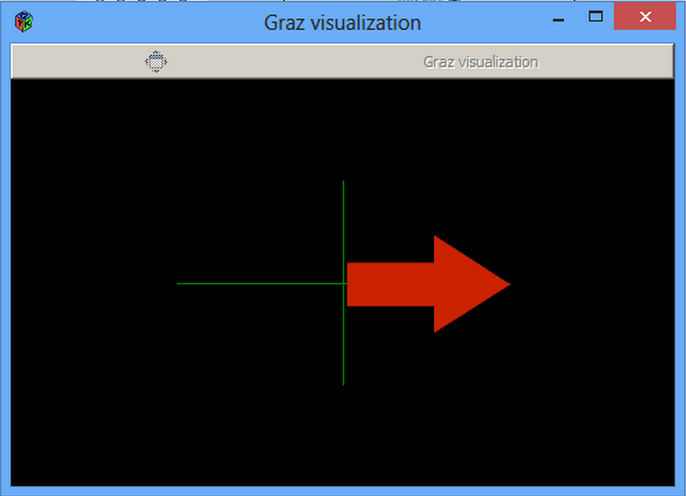
\includegraphics[height=7cm]{images/exempleAcquisition.png}
	\caption[Stimulation visuelle pour l'apprentissage.]{Stimulation visuelle pour l'apprentissage. 40 stimuli visuels sont présentés à l'utilisateur. Lorsque que celui-ci voit une flèche orientée vers la gauche, il doit penser à un mouvement de sa main gauche. Même exercice pour les flèches orientées vers la droite.}
	\label{acqui}
\end{figure}

\begin{figure}[h]
	\centering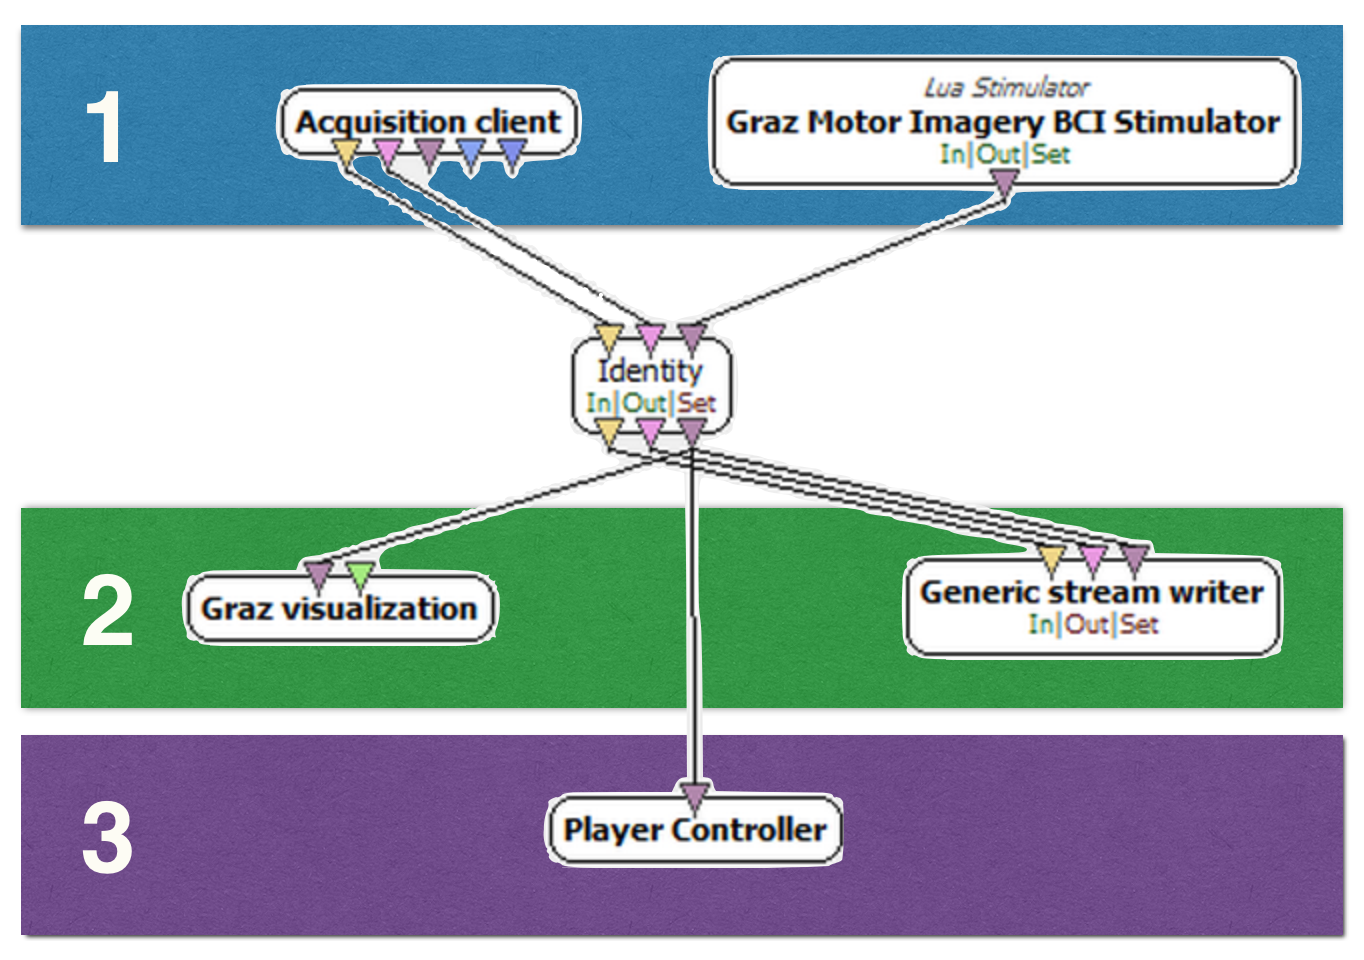
\includegraphics[height=9cm]{images/scenario1.png}
	\caption[Scénario 1 : Acquisition.]{Scénario 1 : Acquisition. Les signaux EEG sont acquis à partir du casque via le bloc "acquisition client". On génère des stimuli visuels grâce au script LUA contenu dans le bloc "Graz Motor Imagery BCI Simulator". Les stimuli sont affichés via le bloc "Graz Visualisation" et " Player Controller". Les données EEG sont quant à elles enregistrées avec le bloc "Generic Stream Writer", générant un fichier .ov}
	\label{scena1}
\end{figure}





\subsection{Scénario 2 : Entrainement du filtre spatial CSP}
\label{Subsection : 6.Scénario 2}
Ce scénario gère l'entrainement du filtre spatial de type CSP (partie \ref{Subsubsecton : 4.CSP})  qui permet de réduire le nombre de canaux (sorties des électrodes) à traiter (Figure \ref{scena2}). Celui-ci fournit en sortie un fichier .cfg. Il s'agit d'un fichier contenant l'ensemble des informations de configuration du filtre CSP (poids attribué à chaque canal).

\textbf{Étapes de déroulement du scénario (Figure \ref{scena2}) : }
\begin{enumerate}
	\item On récupère les signaux EEG bruts et les labels de stimulation enregistrés lors de l'exécution du scénario précédent. 
	\smallbreak
	\item On réalise un filtrage temporel des signaux EEG afin de ne conserver que les rythmes alpha et bêta du cerveau.
	\smallbreak
	\item On découpe les signaux EEG en plusieurs parties, dont leur durée correspond à la durée d'un stimulus visuel. Ces sections sont triées en deux catégories : les signaux correspondant à une réponse à un stimulus gauche (flèche orientée vers la gauche) et les signaux correspondant à une réponse à un stimulus droit (flèche orientée vers la droite).
	\smallbreak
	\item On envoie les deux catégories de signaux vers l'entraineur du filtre CSP.
\end{enumerate}

Il faut environ 8 secondes pour que l'ordinateur calcule les paramètres du filtre (il faut utiliser la fonction de lecture rapide). A la fin de l'exécution du scénario, un message sur le terminal nous informe de la bonne réalisation de la configuration du filtre spatial (Figure \ref{consoleCSP}).

\smallbreak
\textbf{Configuration du bloc "Generic Stream Reader" : }
\smallbreak
\begin{itemize}
	\item File Name .ov : Indiquer le chemin vers le fichier .ov généré lors de l'exécution du scénario précédent, afin de récupérer les signaux EEG bruts et les labels de stimulation correspondants.
	\smallbreak
\end{itemize}

\smallbreak
\textbf{Configuration du bloc "Temporal Filter" : }
\smallbreak
\begin{itemize}
	\item Type de filtre : Butterworth, Passe bande.
	\smallbreak
	\item Fréquences de coupure : 8Hz - 30Hz.
\end{itemize}

\smallbreak
\textbf{Configuration des blocs "Simulation Based Epoching" : }
\smallbreak
\begin{itemize}
	\item Epoch Duration : Se réfère à la durée d'un stimulus visuel produit par le script LUA, afin de découper le signal en plusieurs parties dont la durée correspond à celle du stimulus visuel associé. La durée est ici de 4 secondes.
	\smallbreak
	\item Epoch Offset : Se réfère à la durée entre deux stimuli visuels. La durée est ici de 0.5 secondes.
	\smallbreak
	\item Stimulation to epoch from : Associe les fragments des signaux découpés au label de stimulation. Dans notre cas, il s'agira du label "OVTK\_GDF\_Left" pour les fragments de signaux EEG correspondant aux stimuli de gauche et le label "OVTK\_GDF\_Right" pour les fragments de signaux EEG correspondant aux stimuli de droite.
\end{itemize}

\smallbreak
\textbf{Configuration du bloc "CSP Spatial Filter Trainer" : }
\smallbreak
\begin{itemize}
	\item Spatial Filter Configuration : Indiquer le chemin et le nom du fichier vers lequel le scénario doit enregistrer le fichier de configuration du CSP (extension .cfg). 
	\smallbreak
	\item Filter Dimension : Spécifie le nombre de sorties que l'on souhaite obtenir après le filtrage spatial.
\end{itemize}

\begin{figure}[h]
	\centering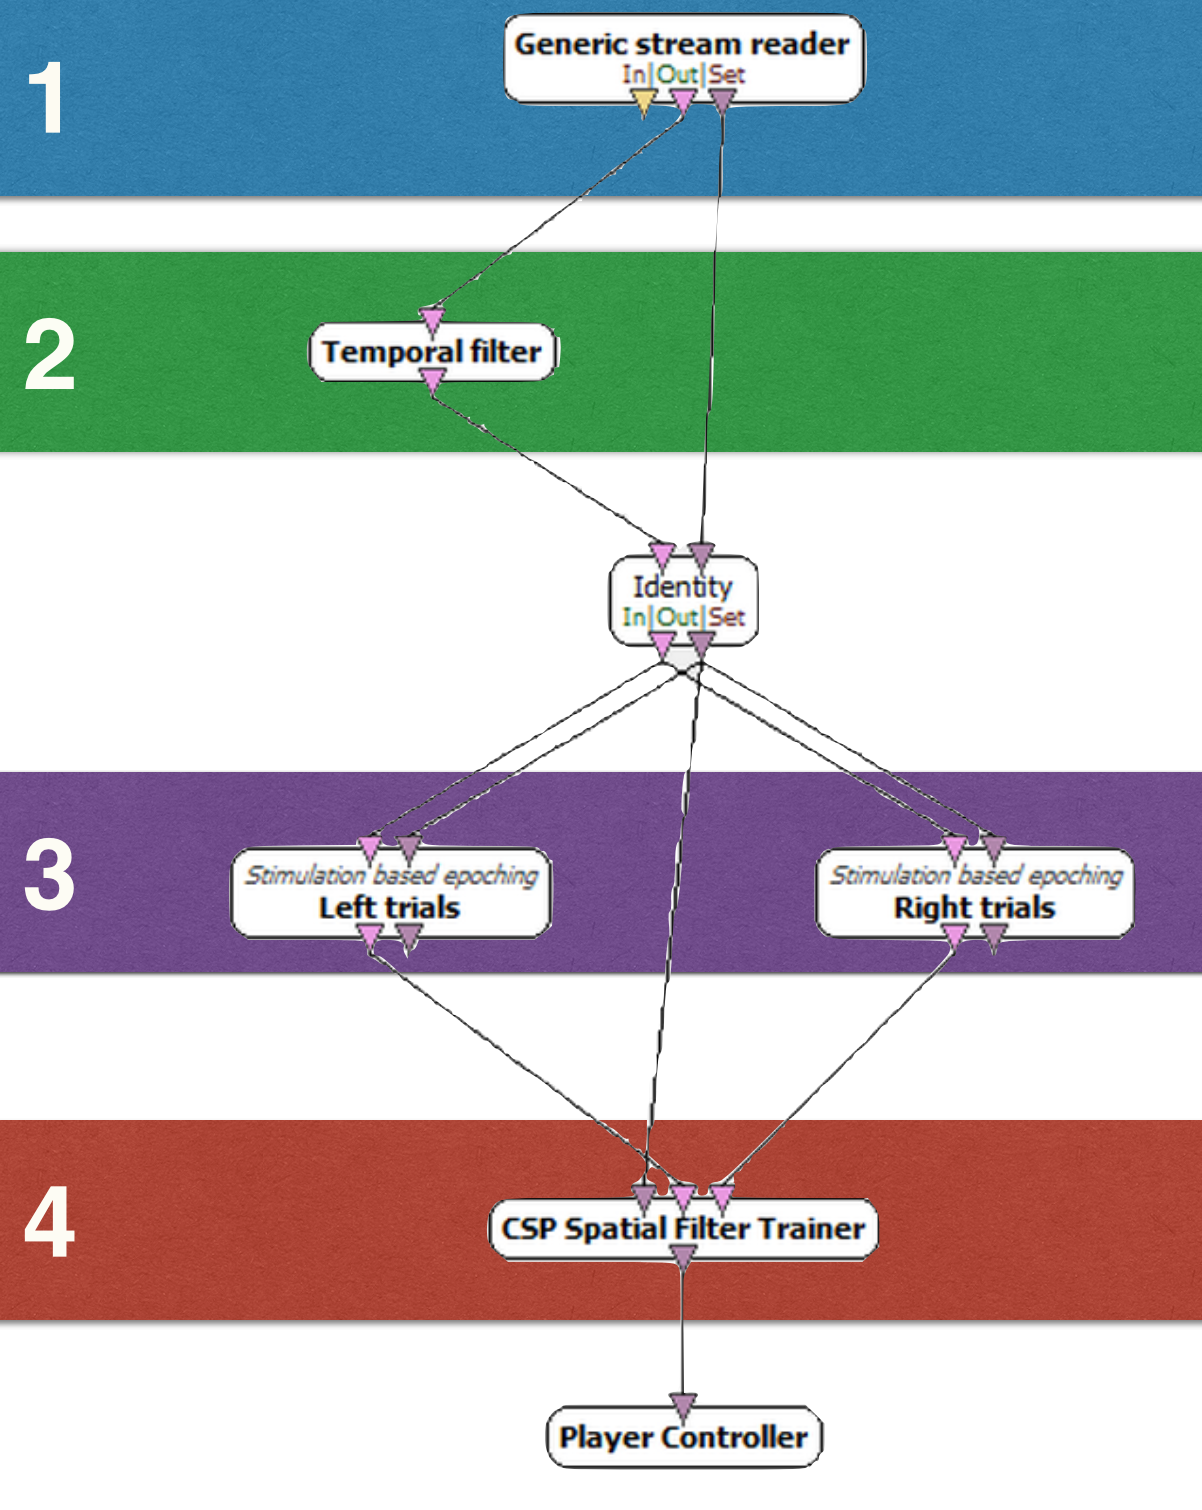
\includegraphics[height=13cm]{images/scenario2.png}
	\caption[Scénario 2 : Entrainement du filtre spatial]{Scénario 2 : Entrainement du filtre spatial. On récupère les données acquises à partir du scénario précédent (bloc "Generic Stream Reader"), puis on réalise un filtrage temporel des signaux EEG afin d'extraire les rythmes alpha et bêta. On découpe et on trie ensuite les signaux EEG en fonction des stimulations visuelles. On entraine le CSP à partir de ces signaux découpés.}
	\label{scena2}
\end{figure}

\begin{figure}[h]
	\centering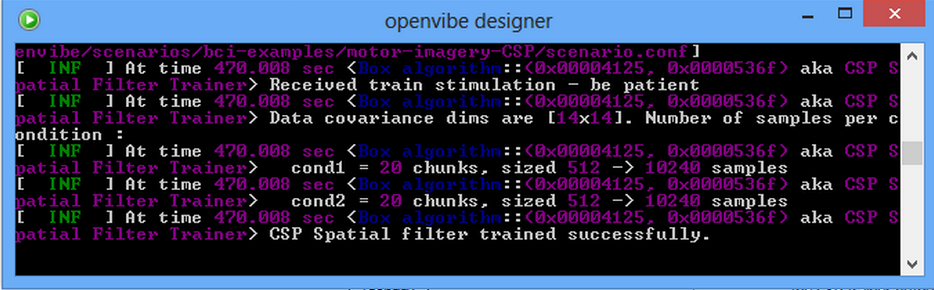
\includegraphics[height=4cm]{images/consoleCSP.png}
	\caption[Sortie console de l'entrainement du CSP]{Sortie console de l'entrainement du CSP. Lorsque l'entrainement du CSP est terminé, le message "CSP Spatial filter trained successfully" apparait.}
	\label{consoleCSP}
\end{figure}





\subsection{Scénario 3 : Entrainement du classificateur}
\label{Subsection : 6.Scénario 3}
Ce scénario sert à entrainer le classificateur LDA (partie \ref{Subsubsection : 4.Linear Discriminant Analysis}) afin que la liaison cerveau-ordinateur soit en mesure de classer les signaux EEG reçus en deux catégories : les signaux correspondants à la pensée de la main gauche, et ceux correspondants à la main droite (Figure \ref{scena3}). Le classificateur se base sur les données acquises lors de l'utilisation du premier scénario et utilise ainsi le fichier .ov qui a été généré. Il utilise également le fichier de configuration obtenu avec l'entrainement du CSP. Le scénario fournit en sortie un fichier .cfg. Il s'agit d'un fichier contenant l'ensemble des informations de configuration du classificateur LDA (Hyperplan et équation du plan).

\smallbreak
\textbf{Étapes de déroulement du scénario (Figure \ref{scena3}) : }
\smallbreak
\begin{enumerate}
	\item On récupère les signaux EEG bruts et les labels de stimulation enregistrés lors de l'exécution du scénario 1. 
	\smallbreak
	\item On réalise un filtrage temporel des signaux EEG afin de ne conserver que les rythmes alpha et bêta du cerveau.
	\smallbreak
	\item On réalise un filtrage spatial de type CSP, à partir de la configuration obtenue dans le scénario précédent. On obtient donc en sortie les canaux sélectionnés et pondérés par le filtre.
	\smallbreak
	\item On découpe les signaux EEG en plusieurs parties, dont leur durée correspond à la durée d'un stimulus visuel. Ces sections sont triées en deux catégories : les signaux correspondant à une réponse à un stimulus gauche (flèche orientée vers la gauche) et les signaux correspondant à une réponse à un stimulus droit (flèche orientée vers la droite).
	\smallbreak
	\item On recoupe de nouveau ces signaux afin d'obtenir des éléments ayant une durée de 1 seconde.
	\smallbreak
	\item On réalise une analyse spectrale en décomposant le signal en série de Fourier. 
	\smallbreak
	\item On place les spectres des signaux dans un vecteur caractéristique.
	\smallbreak
	\item On entraîne le classificateur. 
\end{enumerate}

À la fin de cette opération, un indice de performance est donné dans la console d'OpenViBE. Cet indice doit être supérieur à 65\% si l'on veut espérer obtenir des résultats cohérents lorsque la liaison cerveau-ordinateur fonctionnera en temps réel, i.e. lors de l'execution du scénario 4 (Figure \ref{consoleClassifier}). Dans le cas contraire, il faut recommencer là partir de la phase d'acquisition (Scénario 1) pour obtenir un meilleur résultat.

\smallbreak
\textbf{Configuration du bloc "Generic Stream Reader" : }
\smallbreak
\begin{itemize}
	\item File Name .ov : Indiquer le chemin vers le fichier .ov généré lors de l'exécution du scénario 1, afin de récupérer les signaux EEG bruts et les labels de stimulation correspondants.
	\smallbreak
\end{itemize}

\smallbreak
\textbf{Configuration du bloc "Temporal Filter" : }
\smallbreak
\begin{itemize}
	\item Type de filtre : Butterworth, Passe bande.
	\smallbreak
	\item Fréquences de coupure : 8Hz - 30Hz.
\end{itemize}

\smallbreak
\textbf{Configuration du bloc "CSP Spatial Filter" : }
\smallbreak
\begin{itemize}
	\item Sélectionner l'option "Override setting with configuration file" puis indiquer le chemin vers le fichier de configuration du CSP généré lors du scénario précédent. Les paramètres "Spatial Filter Coefficients", "Number of Output Channels" et "Number of Input Channels" se configurent alors automatiquement. 
\end{itemize}

\smallbreak
\textbf{Configuration des blocs "Simulation Based Epoching" : }
\smallbreak
\begin{itemize}
	\item Epoch Duration : Se réfère à la durée d'un stimulus visuel produit par le script LUA, afin de découper le signal en plus parties dont la durée correspond à celle du stimulus visuel associé. La durée est ici de 4 secondes.
	\smallbreak
	\item Epoch Offset : Se réfère à la durée entre deux stimuli visuels. La durée est ici de 0.5 secondes.
	\smallbreak
	\item Stimulation to epoch from : associe les fragments de signaux découpés au label de stimulation. Dans notre cas, il s'agira du label "OVTK\_GDF\_Left" pour les fragments de signaux EEG correspondant aux stimuli de gauche et le label "OVTK\_GDF\_Right" pour les fragments de signaux EEG correspondant aux stimuli de droite.
\end{itemize}

\smallbreak
\textbf{Configuration du bloc "Time Based Epoching" : }
\smallbreak
\begin{itemize}
	\item Epoch 1 duration : Correspond à la durée des tranches de signaux. 1 seconde dans le cas présent.
	\smallbreak
	\item Epoch 1 intervals : Intervalle de temps entre chaque tranche de signal. 0.0625 secondes dans le cas présent. 
\end{itemize}

\smallbreak
\textbf{Configuration du bloc "Spectral analysis (FFT)" : }
\smallbreak
\begin{itemize}
	\item Spectral components : Permet de sélectionner la composante spectrale analysée. On souhaite ici utiliser le spectre d'amplitude du signal. 
\end{itemize}

\smallbreak
\textbf{Configuration du bloc "Spectrum Average" : }
\smallbreak
\begin{itemize}
	\item Ne requière pas de configuration particulière.
\end{itemize}

\smallbreak
\textbf{Configuration du bloc "Classifier trainer" : }
\smallbreak
\begin{itemize}
	\item Train Trigger : Permet de sélectionner le drapeau permettant de démarrer l'entrainement du classificateur. Il s'agit ici du drapeau "OVTK\_Stimulationid\_Train qui est généré par les données de stimulation provenant du bloc "Generic stream reader".
	\smallbreak
	\item Filename to save configuration to : Permet de sélectionner le répertoire et le nom sous lequel enregistrer le fichier de configuration du classificateur (extension .cfg).
	\smallbreak
	\item Class 1 label : Sélectionne le label de la classe 1. Il s'agira ici du label utilisé pour la stimulation gauche (flèche orientée à gauche) "OVTK\_GDF\_Left".
	\smallbreak
	\item Class 2 label : Sélectionne le label de la classe 2. Il s'agira ici du label utilisé pour la stimulation droite (flèche orientée à droite) "OVTK\_GDF\_Right".
	\smallbreak 
	\item Algorithm to use : Permet de sélectionner le type de classification à réaliser (LDA ou SVM). On décide ici d'utiliser un classificateur LDA.
\end{itemize}

\begin{figure}[h]
	\centering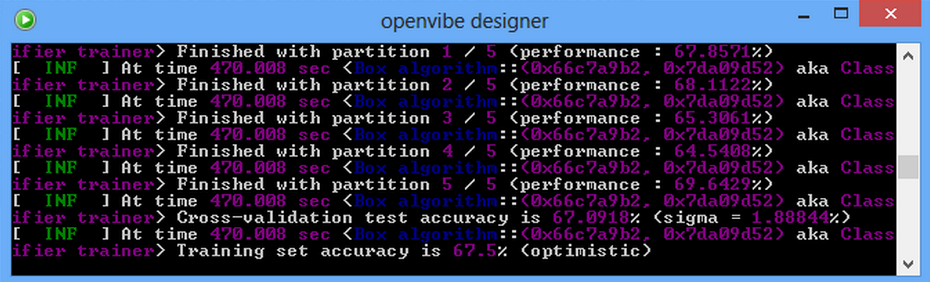
\includegraphics[height=4cm]{images/consoleClassifier.png}
	\caption[Sortie console résultant de l'entrainement du classificateur.]{Sortie console résultant de l'entrainement du classificateur. Une valeur correspondant en pourcentage à la précision de l'entraînement de la classification nous est fournie.}
	\label{consoleClassifier}
\end{figure}

\begin{figure}[h]
	\centering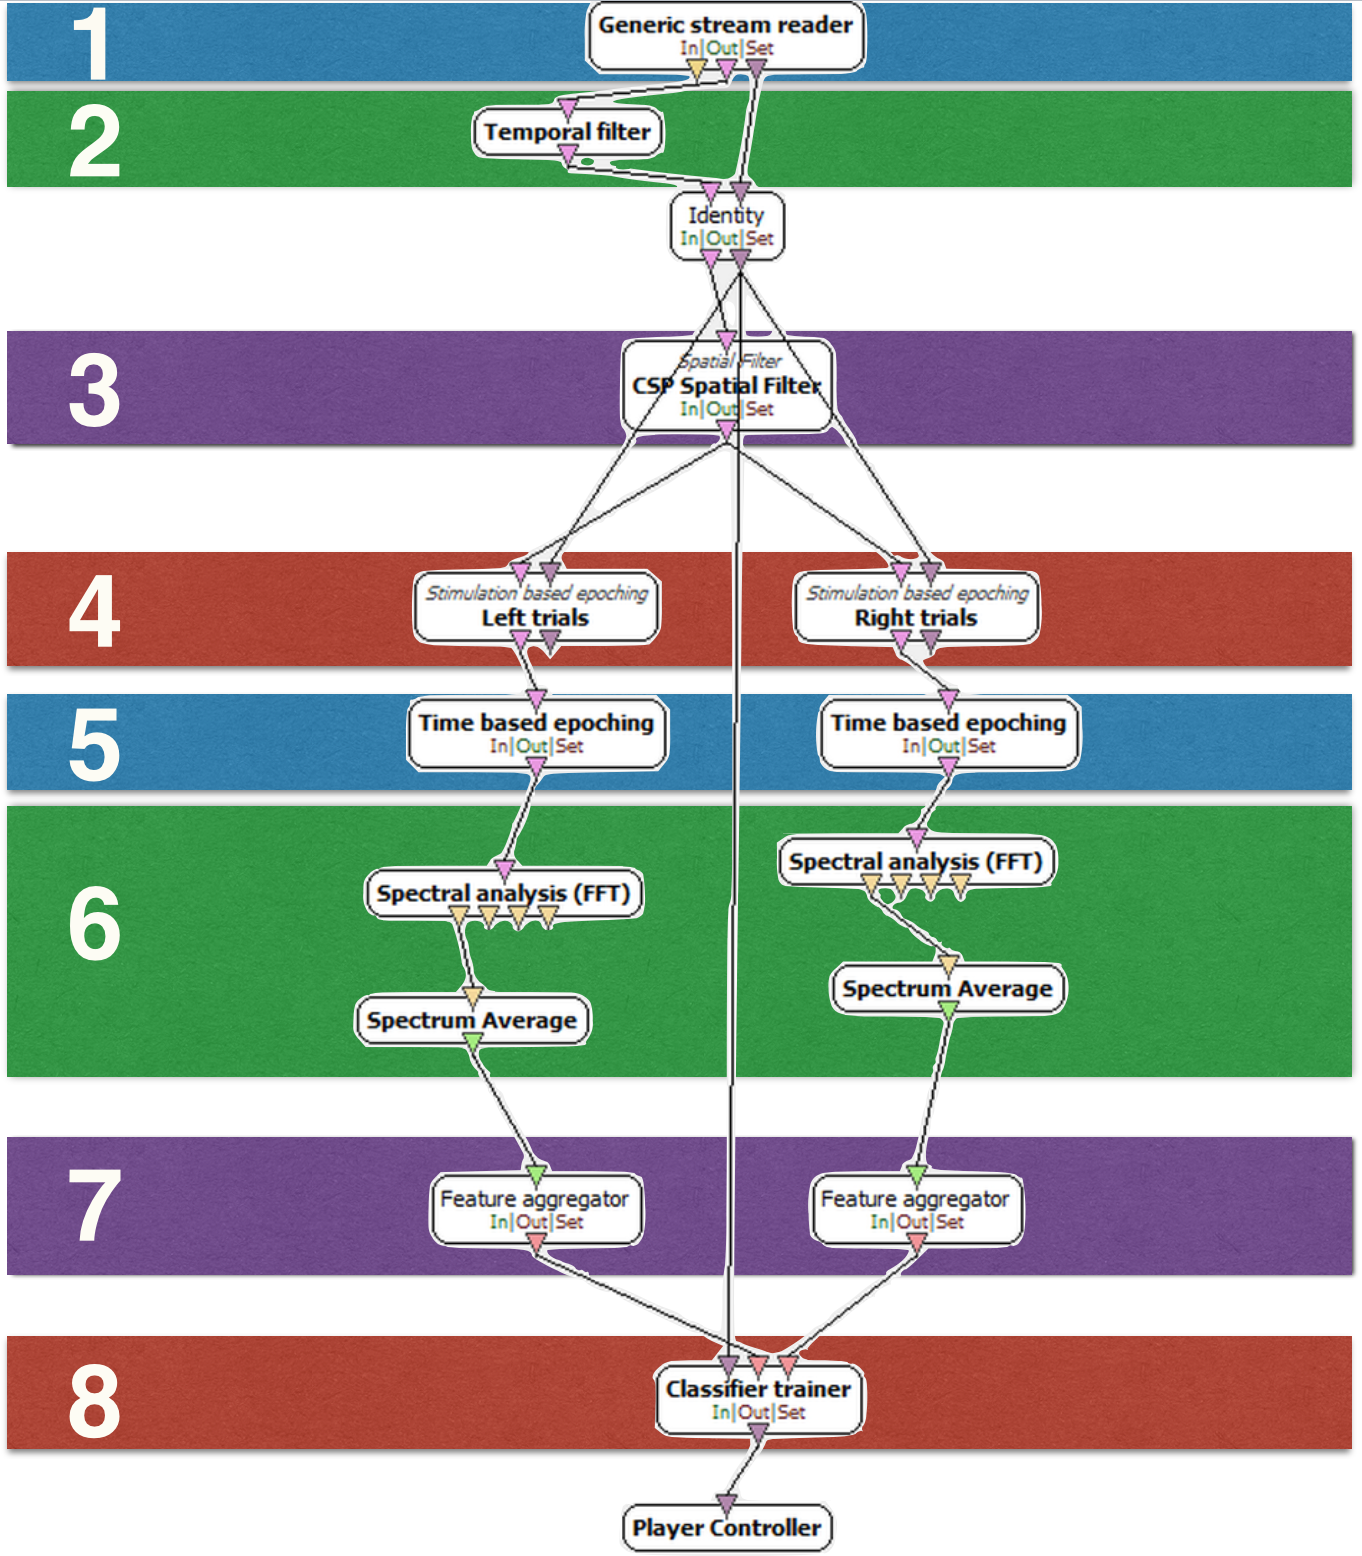
\includegraphics[height=16cm]{images/scenario3.png}
	\caption[Scénario 3 : Entrainement du classificateur]{Scénario 3 : Entrainement du classificateur. A partir des signaux acquis lors du scénario 1, on vient entrainer le classificateur en vu de l'utiliser pour le scénario 4 (temps réel). Pour cela, on commence par filtrer des signaux d'entrée afin d'extraire les signaux alpha et bêta du cerveau. Puis on réalise un filtrage spatial grâce au filtre CSP entrainé lors du scénario précédent. Enfin on effectue un analyse spectral des signaux filtrés pour les présenter en entrée de l'entraineur du classificateur.}
	\label{scena3}
\end{figure}








\subsection{Scénario 4 : Utilisation en temps réel de l'interface}
\label{Subsection : 6.Scénario 4}
Ce scénario permet d'utiliser la liaison cerveau-ordinateur en temps réel. Il s'appuie sur les configurations effectuées grâce aux scénarios précédents, i.e. le filtre spatial CSP et classificateur LDA (Figure \ref{scena4}). On place dans le scénario un certain nombre de blocs permettant de visualiser les résultats obtenus ("Signal display, "Power spectrum display", "Post CSP display", "Graz Visualisation").

\textbf{Étapes de déroulement du scénario (Figure \ref{scena3}) : }
\begin{enumerate}
	\item On récupère les signaux EEG  à partir du casque EPOC, en temps réel (Figure : \ref{xpBrut}).
	\smallbreak 
	\item On réalise un filtrage temporel des signaux EEG afin de ne conserver que les rythmes alpha et bêta du cerveau (Figure : \ref{xpFiltered}).
	\smallbreak
	\item On réalise un filtrage spatial de type CSP, à partir de la configuration obtenue dans le scénario 2. On obtient donc en sortie les canaux sélectionnés et pondérés par le filtre (Figure : 	\ref{xpCsp}).
	\smallbreak
	\item On découpe les signaux afin d'obtenir des tranches de signal ayant une durée de 1 seconde.
	\smallbreak
	\item On réalise une analyse spectrale en décomposant le signal en série de Fourier (Figure : \ref{xpPowerSpectrum}).
	\smallbreak
	\item On place les spectres des signaux dans un vecteur caractéristique.
	\smallbreak
	\item On réalise la classification des données à partir du classificateur entrainé grâce au scénario précédent. On obtient donc en sortie l'estimation du système quant à la pensée de l'utilisateur (Figure : \ref{online}).
\end{enumerate}

\smallbreak
\textbf{Configuration du bloc "Acquisition Client" : }
\smallbreak
\begin{itemize}
	\item Acquisition Server HostName : "\${AcquisitionServer\_HostName}".
	\smallbreak
	\item Acquisition Server Port : Port de connexion correspondant au casque Epoc. Valeur par défaut 1024.
\end{itemize}

\smallbreak
\textbf{Configuration du bloc "Temporal Filter" : }
\smallbreak
\begin{itemize}
	\item Type de filtre : Butterworth, Passe bande.
	\smallbreak
	\item Fréquences de coupure : 8Hz - 30Hz.
\end{itemize}

\smallbreak
\textbf{Configuration du bloc "CSP Spatial Filter" : }
\smallbreak
\begin{itemize}
	\item Sélectionner l'option "Override setting with configuration file" puis indiquer le chemin vers le fichier de configuration du CSP généré lors du scénario précédent. Les paramètres "Spatial Filter Coefficients", "Number of Output Channels" et "Number of Input Channels" se configurent alors automatiquement. 
\end{itemize}

\smallbreak
\textbf{Configuration du bloc "Time Based Epoching" : }
\smallbreak
\begin{itemize}
	\item Epoch 1 duration : Correspond à la durée des tranches de signaux. 1 seconde dans le cas présent.
	\smallbreak
	\item Epoch 1 intervals : Intervalle de temps entre chaque tranches de signal. 0.0625 secondes dans le cas présent. 
\end{itemize}

\smallbreak
\textbf{Configuration du bloc "Spectral analysis (FFT)" : }
\smallbreak
\begin{itemize}
	\item Spectral components : Permet de sélectionner la composante spectrale analysée. On souhaite ici utiliser le spectre d'amplitude du signal. 
\end{itemize}

\smallbreak
\textbf{Configuration du bloc "Spectrum average" : }
\smallbreak
\begin{itemize}
	\item Ne requière pas de configuration particulière.
\end{itemize}

\smallbreak
\textbf{Configuration du bloc "Classifier processor" : }
\smallbreak
\begin{itemize}
	\item Filename to load configuration from : Indiquer le chemin vers le fichier de configuration généré lors de l'exécution du scénario précédent.
\end{itemize}

\begin{figure}[h]
	\centering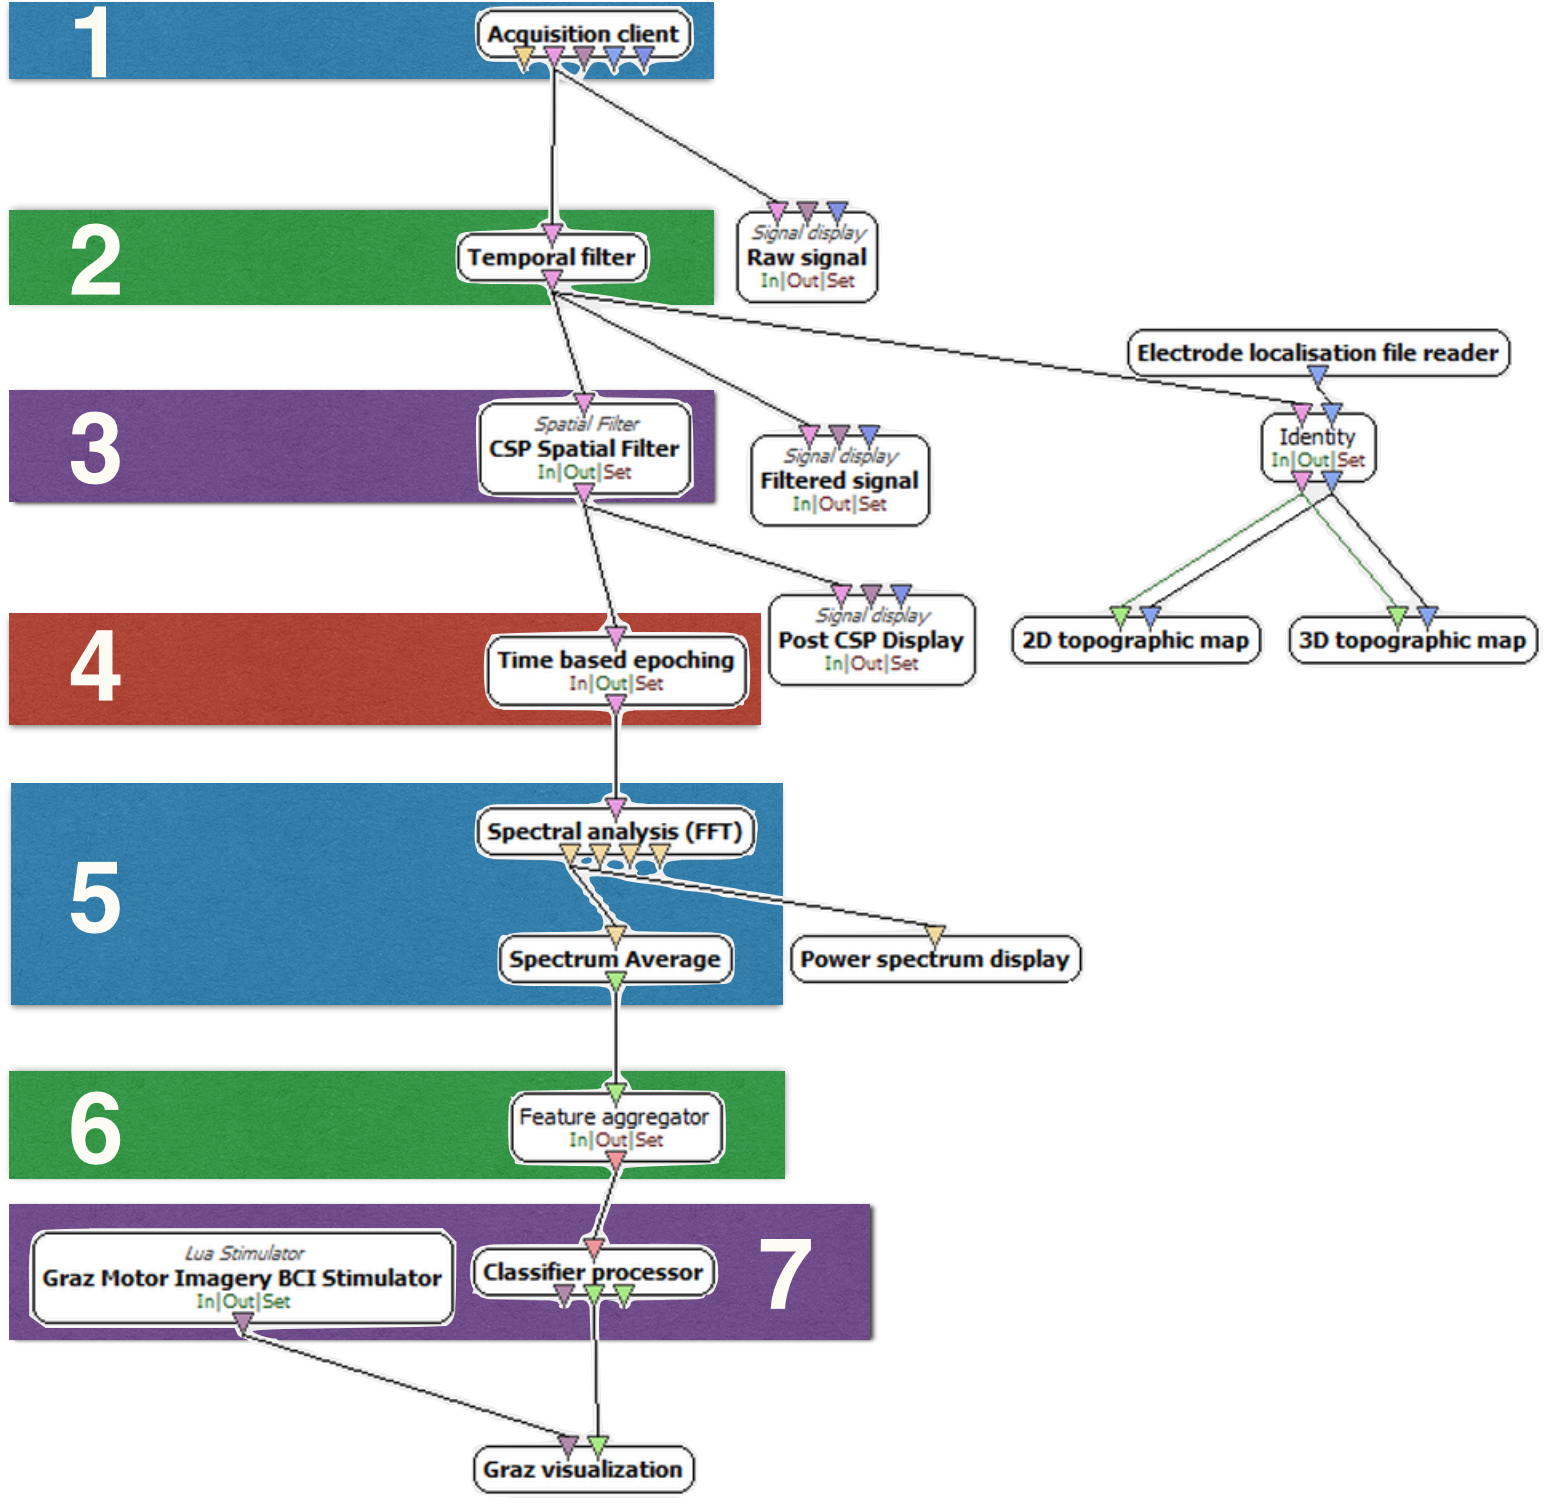
\includegraphics[height=16cm]{images/scenario4.png}
	\caption[Scénario 4 : Utilisation en temps réel]{Scénario 4 : Utilisation en temps réel. Celui-ci permet d'utiliser la liaison cerveau-ordinateur en temps réel. Pour cela, on enregistre en entrée les signaux provenant en temps réel du casque (bloc "acquisition client"). On effectue par la suite un filtrage temporel afin d'extraire les rythmes alpha et bêta du cerveau. On réalise à partir de ces rythmes un filtrage CSP afin de réduire le nombre de signaux en sortie. Une analyse spectrale est ensuite réalisée afin d'effectuer une classification LDA. Les données sont visualisées via les différents bloc de visualisation.}
	\label{scena4}
\end{figure}





\section {Résultats obtenus et analyse}
\label{Section : 6.Résultats obtenus et analyse}
Au départ, notre première expérience utilisait un filtre statique de type Laplacien. Or, les résultats obtenus n'étaient pas satisfaisant (55\% de performances environ). Après remplacement du filtre statique par un filtre spatial par apprentissage de type CSP, on obtient de meilleurs performances. (75 à 80 \% de performance avec le filtre CSP).

Deux facteurs principaux altèrent la qualité des résultats :
\smallbreak
\begin{itemize}
	\item \textbf{Qualité des signaux d'entrée.} Un mauvais positionnement du casque sur le crâne ou une mauvaise hydratation des électrodes peut réduire la qualité des signaux entrant dans le système, réduisant ainsi la qualité des résultats.
	\smallbreak
	\item \textbf{Concentration de l'utilisateur.}  L'exécution du premier scénario nécessite une concentration importante de l'utilisateur. En effet, si celui-ci ne se concentre pas suffisamment sur les stimuli visuels et sur sa représentation visuelle du mouvement de ses main, la qualité de la classification sera altérée. De même si l'individu parle ou bouge durant l'acquisition des données.
\end{itemize}


\begin{figure}[h]
	\centering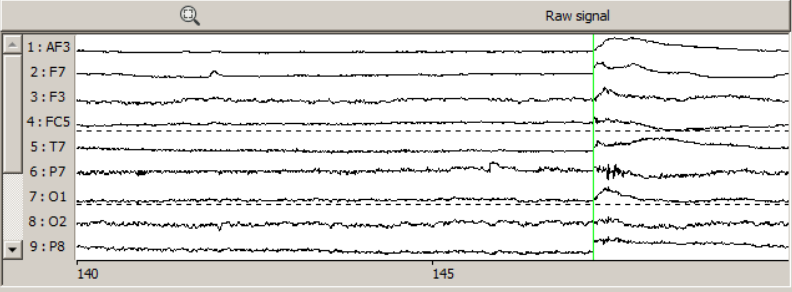
\includegraphics[height=4cm]{images/xpRawSignal.png}
	\caption[Signaux bruts observés en sortie du casque Emotiv]{Signaux bruts observés en sortie du casque Emotiv, sur les 14 canaux (électrodes).}
	\label{xpBrut}
\end{figure}

\begin{figure}[h]
	\centering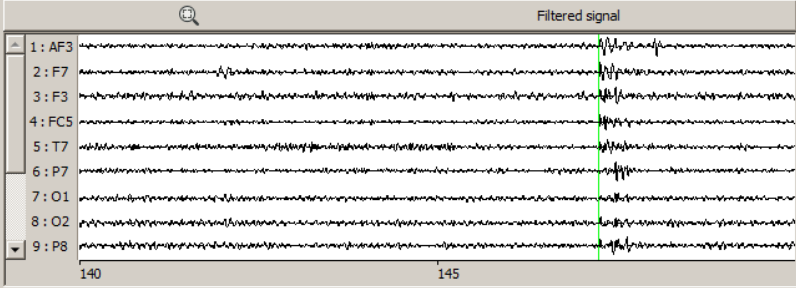
\includegraphics[height=4cm]{images/xpFilteredSignal.png}
	\caption[Signaux filtrés]{Signaux filtrés temporellement afin d'extraire les rythmes alpha et bêta du cerveau.}
	\label{xpFiltered}
\end{figure}

\begin{figure}[h]
	\centering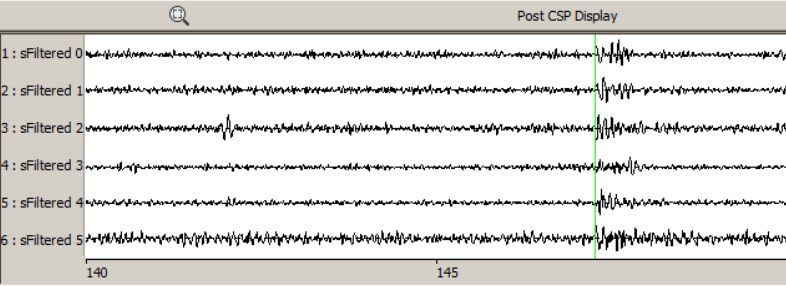
\includegraphics[height=4cm]{images/xpCsp.png}
	\caption[Réduction du nombre de sorties grâce au filtrage CSP]{Réduction du nombre de sorties grâce au filtrage CSP. On passe de 14 entrées à 6 sorties.}
	\label{xpCsp}
\end{figure}

\begin{figure}[h]
	\centering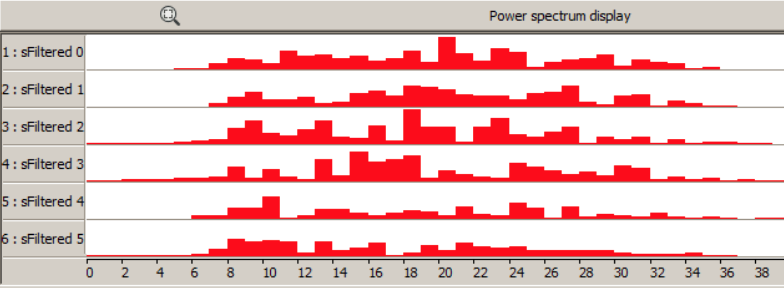
\includegraphics[height=4cm]{images/xpPowerSpectrum.png}
	\caption[Analyse spectrale des signaux]{Analyse spectrale des signaux via une transformation de Fourier.}
	\label{xpPowerSpectrum}
\end{figure}

\newpage
\begin{figure}[h]
	\centering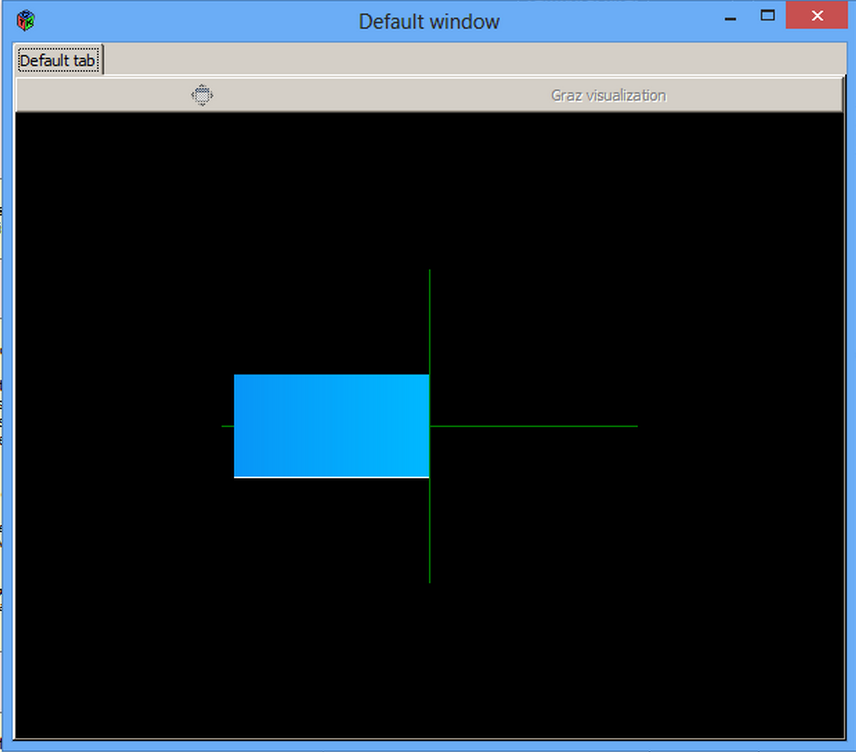
\includegraphics[height=10cm]{images/online.png}
	\caption[Sortie visuelle temps réel après classification]{Sortie visuelle temps réel après classification. La direction du curseur bleu correspond à la pensée de l'utilisateur : Si le curseur se dirige vers la gauche, cela signifie que le système estime que la personne pense à un mouvement de sa main gauche. Si au contraire le curseur se dirige vers la droite, cela signifie que le système estime que la personne pense à un mouvement de sa main droite. Plus le curseur s'éloigne du centre de l'image, plus la certitude du système est élevée.}
	\label{online}
\end{figure}
  \chapter{Intégration du projet dans le cadre de cours}
\thispagestyle{fancy}

On souhaite intégrer notre projet dans le cadre de plusieurs cours enseignés par Jean Rouat.
\smallbreak
\begin{itemize}
	\item \textbf{Cours gradué de techniques avancées en traitement des signaux.} Ce cours enseigne les différentes méthodes de représentation d'un signal dans le domaine spectral (transformée de Fourier, transformation en ondelettes, etc.), ainsi que les outils de filtrage spectral (Analyse en composantes principales, analyse en composantes indépendantes). Cours enseigné à la session d'automne. 
	\smallbreak
	\item\textbf{APP d'intelligence probabiliste}. Ce cours s'intéresse aux différentes méthodes de classification, et notamment les méthodes paramétriques (Bayesiennes) et non paramétriques (k-moyen, SVM, etc.). Cours enseigné à la session d'automne.
	\smallbreak
	\item \textbf{Cours de neurosciences computationnelles}. Ce cours enseigne les principes de base de la physiologie des réseaux neuronaux et leurs modélisations. Il offre également une vision d'ensemble des différents domaines d'application. Cours enseigné à la session d'hiver.
\end{itemize} 

On propose donc différents travaux pratiques permettant aux étudiants de mettre en application leurs connaissances acquises au cours de la matière.

\section{Choix des outils mathématiques d'apprentissage}

Afin d'intégrer notre liaison cerveau-ordinateur dans les différents cours, on souhaite exporter les données traitées dans OpenViBE vers un environnement de développement mathématique, afin que les élèves puissent travailler sur les signaux. Trois environnements s'offrent à nous : 
\smallbreak
\begin{itemize}
	\item \textbf{Matlab}. Il s'agit d'un langage de programmation haut niveau, associé à un environnement de développement portant le même nom. L'avantage de cet outil est qu'il est assez simple à appréhender et que la plupart des étudiants l'ont déjà utilisé à de nombreuses reprises. OpenViBE offre la possibilité d'exécuter du code Matlab sous son environnement et de l'utiliser dans la chaine de traitement des signaux EEG. Cela nécessite cependant d'utiliser Matlab 32 bits sur les ordinateurs des laboratoires, or ceux-ci possèdent uniquement la version 64 bits. Un autre de ses inconvénients 
	est qu'il s'agit d'un logiciel payant.  
	\smallbreak
	\item \textbf{Octave.} Octave est un langage de programmation mathématique de haut-niveau. Il a l'avantage d'être totalement gratuit. Cependant, OpenViBE ne propose aucune solution d'intégration d'Octave directement dans l'interface du logiciel.
	\smallbreak
	\item \textbf{Python.} Il s'agit d'un langage de programmation haut-niveau. OpenViBE propose une solution d'intégration de Python dans son environnement afin de l'utiliser dans la chaine de traitement des signaux. Cependant, cette intégration est complexe à mettre en place et nécessite de la part des élèves des connaissances autre que la simple maitrise du langage. 
\end{itemize}
\smallbreak
Aucun des environnement proposés ne semble être intégrable directement dans OpenViBE. On propose donc comme alternative d'exporter les données traitées sous OpenViBE vers un fichier CSV. Ce format représente des données tabulaires sous forme de valeurs séparées par des virgules. Il a donc l'avantage d'être lisible directement par l'Homme et de nombreux logiciels de traitement de données, comme Matlab ou même Excel. Nous proposons donc d'utiliser Matlab comme environnement de travail pour la réalisation des travaux pratiques.

\section{Cours de neurosciences computationnelles}

\subsection{Résumé du travail pratique proposé}

Le travail pratique que nous proposons aux étudiants dans le cadre du cours de neurosciences computationnelles correspond plus à un travail d'observation et de compréhension des différentes étapes de traitement des signaux électroencéphalographiques. On leur demande d'étudier le lien entre les connaissances physiologiques acquises lors du cours et les différents aspects techniques de l'interface cerveau-ordinateur. 

Pour cela, on fournit le scénario 4 (Figure \ref{scenario_neuro}) réalisé dans le cadre de l'expérience simple (partie \ref{Chapitre : Première exprérience simple d'interaction}). L'entrainement du classificateur et du filtre spatial CSP ayant été réalisé en amont, on demande donc aux étudiants de s'intéresser uniquement à l'exécution en temps réel de l'interface cerveau-ordinateur. Plusieurs outils de visualisation ont été intégré au scénario, afin que les étudiants puissent observer l'activité cérébrale (Figure \ref{cours_neuro}): 

\begin{itemize}
	\item \textbf{2D topographic map.} Permet d'observer l'activité cérébrale de l'individu portant le casque sur une représentation en 2 dimensions du crâne.
	\smallbreak
	\item \textbf{3D topographic map.} Permet d'observer l'activité cérébrale de l'individu portant le casque sur une représentation en 3 dimensions du crâne.
	\smallbreak
	\item \textbf{Signal display.} Permet d'observer les signaux EEG à différentes étapes de leur traitement (en sortie du casque EEG, après filtrage temporel).
	\smallbreak
	\item \textbf{Post CSP Display.} Permet d'observer les signaux et plus particulièrement la sélection des canaux (signaux de sortie des électrodes) après le filtrage spatial de type CSP.
	\smallbreak
	\item \textbf{Power spectrum display.} Permet d'observer les différents spectres des signaux après transformation en série de Fourier. 
	\smallbreak
	\item \textbf{Graz Visualisation.} Permet d'observer les résultats de l'expérience après classification des données.
\end{itemize}

\begin{figure}[h]
	\centering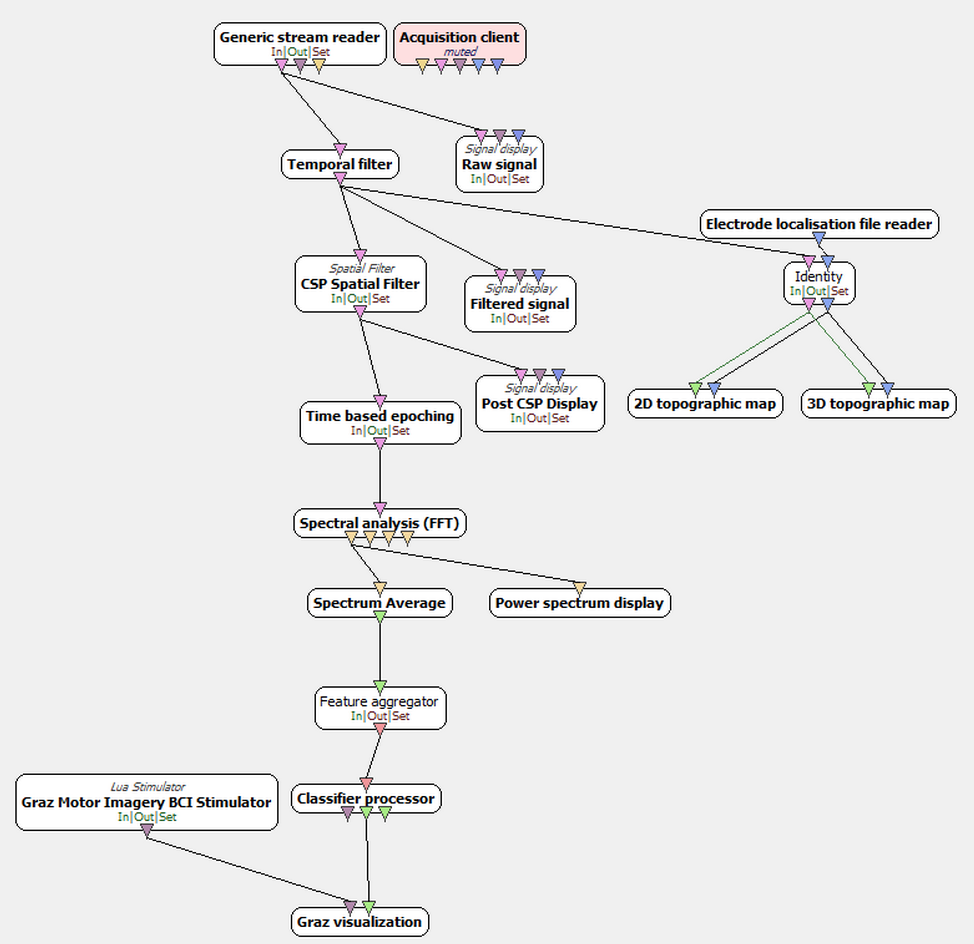
\includegraphics[height=15cm]{images/scenario_neuro.png}
	\caption[Scénario temps réel proposé dans le cadre du cours de neurosciences computationnelles.]{Scénario temps réel proposé dans le cadre du cours de neurosciences computationnelles.}
	\label{scenario_neuro}
\end{figure}

\begin{figure}[h]
	\centering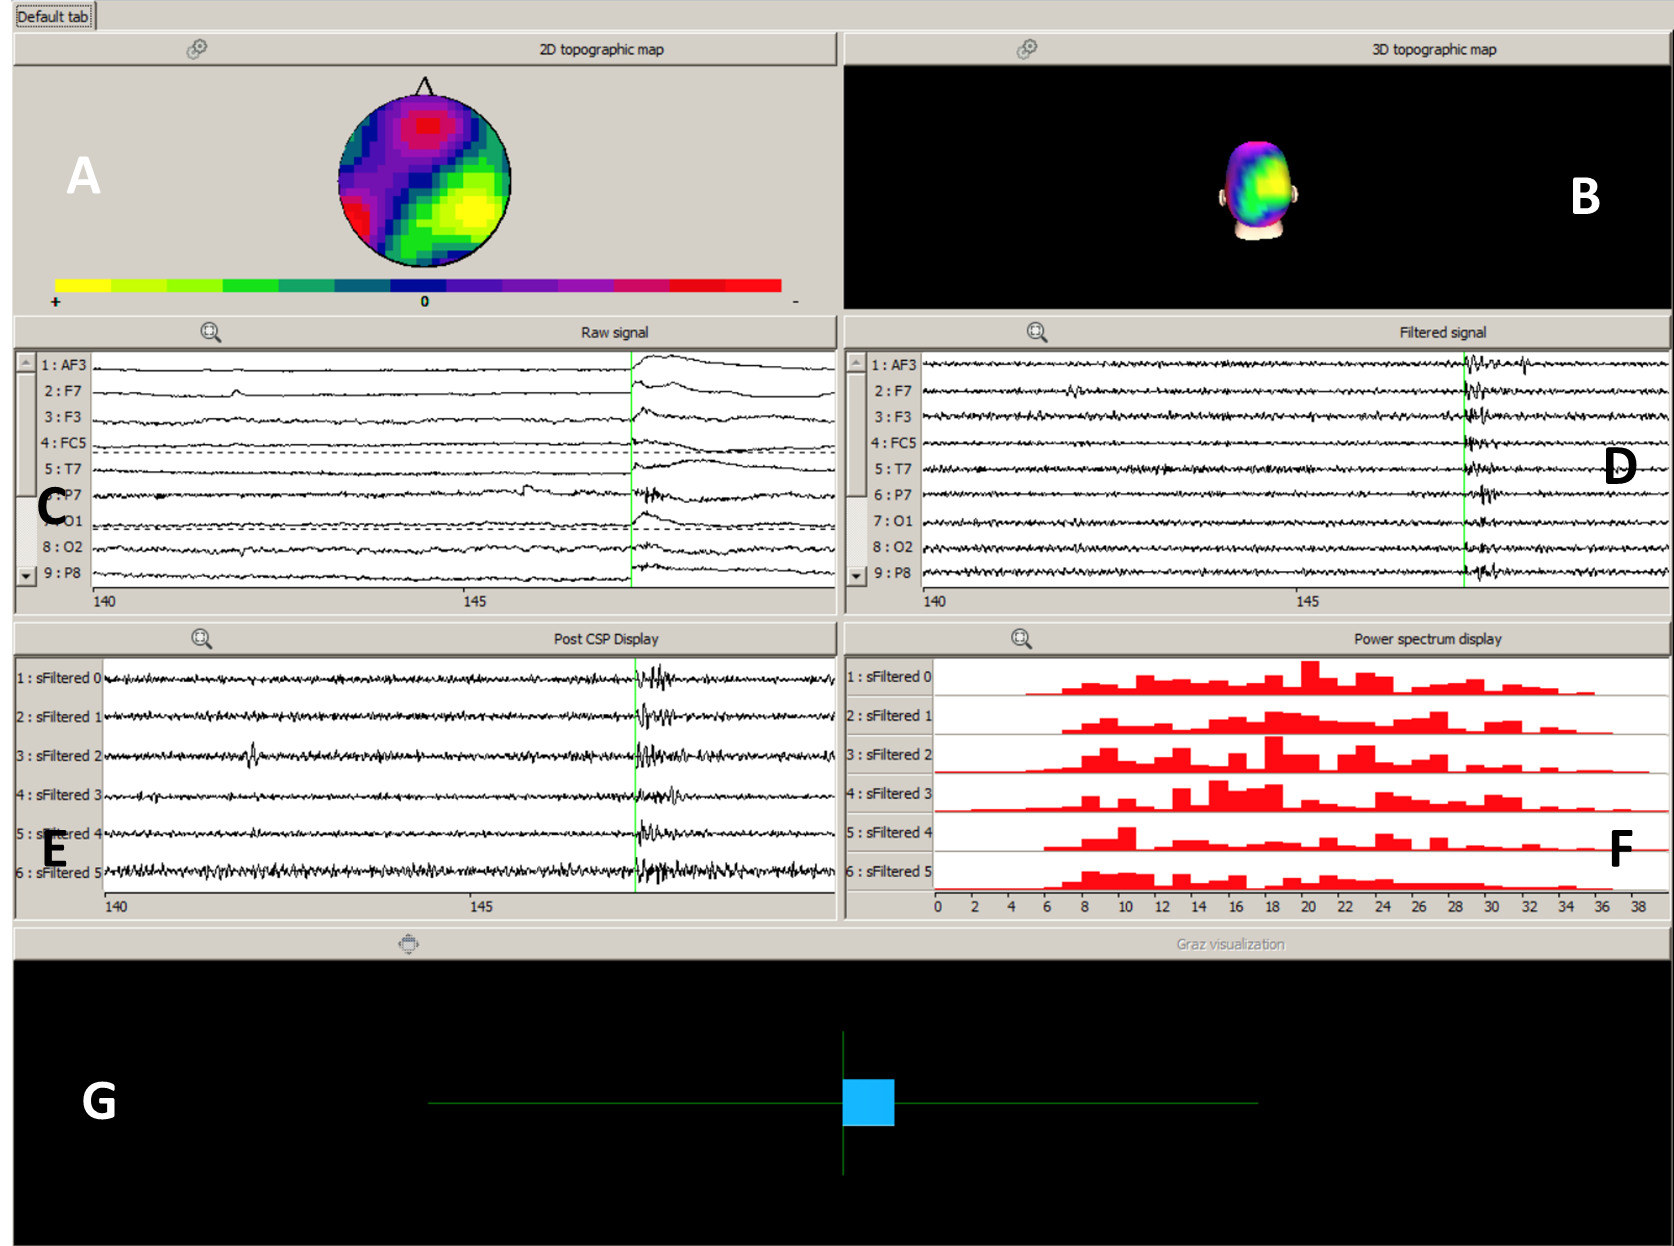
\includegraphics[height=12cm]{images/cours_neuro.png}
	\caption[Interface de visualisation proposée aux étudiants du cours de neurosciences]{Interface de visualisation proposée aux étudiants du cours de neurosciences. (A) Visualisation topographique de l'activité cérébrale en 2D. (B) Visualisation topographique de l'activité cérébrale en 3D. (C) Visualisation des signaux en sortie du casque, i.e. les signaux non traités. (D) Visualisation des signaux après filtrage temporel. (E) Visualisation des signaux après filtrage spatial CSP. (F) Visualisation des spectres fréquentiels après FFT. (G) Fenêtre de visualisation  }
	\label{cours_neuro}
\end{figure}

\subsection{Préparation du travail pratique par le professeur}

Le TP reposant uniquement sur le scénario 4, on propose ici deux approches pour la préparation du cours de neurosciences.

\subsubsection{Travail en groupe}

\begin{enumerate}
	\item Le professeur réalise en amont l'acquisition des signaux EEG (scénario 1), l'entrainement du filtre CSP (scénario 2) et l'entrainement du classificateur LDA (scénario 3).
	\smallbreak
	\item La classe ne disposant que d'un seul casque, le professeur exécutera devant l'ensemble des élèves le scénario 4 en l'utilisant grâce au bloc "Acquisition Client". Cela nécessite donc de configurer préalablement OpenViBE et le casque EPOC comme présenté en partie \ref{Chapitre : Utilisation du casque EPOC et d'OpenViBE}.
	\smallbreak
	\item  Les fichiers de configuration générés par les scénarios 2 et 3 sont utilisés pour exécuter le  scénario 4 lors du cours. Pour cela, on renseigne le chemin vers les fichiers de configuration dans les blocs "CSP spatial Filter" et "Classifier Processor".
	\smallbreak
	\item Vérifier dans le bloc "Graz Visualisation" que la case "Show instruction" est bien décochée.
\end{enumerate}

\subsubsection{Travail individuel}

\begin{enumerate}
	\item Les élèves sont dans un premier temps invités à télécharger OpenViBE.
	\smallbreak
	\item On fournit alors à l'ensemble des élèves le scénario 4, ainsi que les fichiers de configuration du filtre spatial CSP et du classificateur LDA, générés par nos soins.
	\smallbreak
	\item La classe ne disposant que d'un casque, on propose d'utiliser en entrée du scénario 4 un fichier contenant un enregistrement de signaux EEG (extension .ov), lisible avec le bloc "Generic Stream Reader". Chaque élève peut alors réaliser individuellement le travail pratique. 
	\smallbreak
	\item Vérifier dans le bloc "Graz Visualisation" que la case "Show instruction" est bien cochée, afin que l'élève puisse visualiser les consignes que l'individu avait en entrée lors de l'enregistrement. 
\end{enumerate}
  

Un sujet de travail pratique à destination des élèves a été rédigé et placé en annexe. Il contient la procédure pour réaliser la manipulation, ainsi que des questions portant sur l'interface cerveau-ordinateur. 

\section{Cours de traitement de signal avancé}

\subsection{Résumé du travail pratique proposé}

Le travail pratique que nous proposons aux étudiants du cours de traitement du signal avancé consiste à réaliser une partie de la chaine de traitement des signaux EEG de l'expérience (partie \ref*{Chapitre : Première exprérience simple d'interaction}), sous l'environnement Matlab. L'objectif est de leur permettre de mettre en application leurs connaissances (filtrage spatial, filtrage temporel, FFT). Le reste de la chaîne de traitement étant effectué sous OpenViBE, on exporte donc les données de OpenViBE vers Matlab grâce au format CSV. Une fois les signaux traités sous Matlab, on exporte à nouveaux ces données vers OpenViBE. Cette méthode de transfert entre les deux logiciels nous oblige cependant à ne pas utiliser l'interface cerveau-ordinateur en temps réel. 

\subsection{Développement de nouveaux scénarios}

Pour ce cours, nous avons implémenté trois nouveaux scénarios. Un seul sera présenté aux étudiants, les deux autres servant à la préparation du travail pratique :
\smallbreak
\begin{itemize}
	\item \textbf{Scénario d'acquisition et de filtrage temporel.} (Figure \ref{acqui2}) 
	L'objectif de ce scénario est de pouvoir récupérer les données en sortie des électrodes du casque EEG filtrées temporellement, afin d'en extraire les rythmes alpha et bêta. Son principe de fonctionnement reste le même que le scénario 1 présenté dans la partie \ref{Subsection : 6.Scénario 1}. Les signaux filtrés ainsi que les données de stimulation sont exportées dans deux fichiers au format .csv. Les données de stimulation correspondent aux stimulations visuelles envoyées à l'utilisateur lors de l'enregistrement des données EEG. Le fichier CSV contenant ces données de stimulation sera utilisé par la suite pour l'entrainement du classificateur. Le fichier CSV contenant les données EEG sera quant à lui utilisé à deux reprises, lors de l'entrainement du classificateur et lors de l'execution de la liaison cerveau-ordinateur. 
		\begin{figure}[h]
			\centering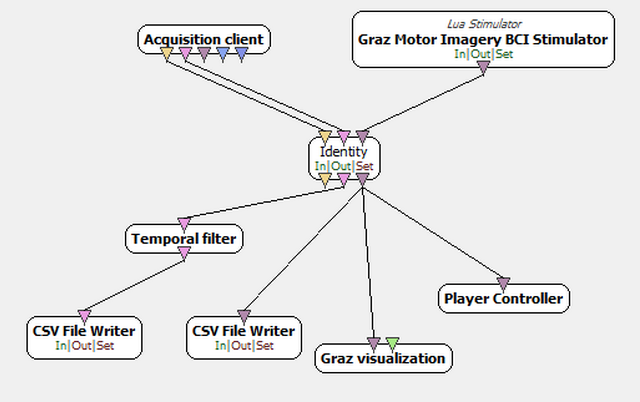
\includegraphics[height=8cm]{images/scenario_2_0.png}
			\caption{Scénario d'acquisition avec sortie au format CSV}
			\label{acqui2}
		\end{figure}
	\smallbreak
	\item \textbf{Scénario d'entrainement du classificateur}. Il permet d'entrainer le classificateur de type LDA (Figure \ref{classi2}).  Le principe de fonctionnement reste identique au scénario présenté dans la partie \ref{Subsection : 6.Scénario 3}. Le scénario nécessite à son entrée deux fichiers CSV. Le premier contient les données reçues du casque lors de la phase d'acquisition après filtrage spatial ICA ou PCA sous Matlab. Le deuxième fichier contient les données de stimulation obtenues lors de la phase d'acquisition.
			\begin{figure}[h]
				\centering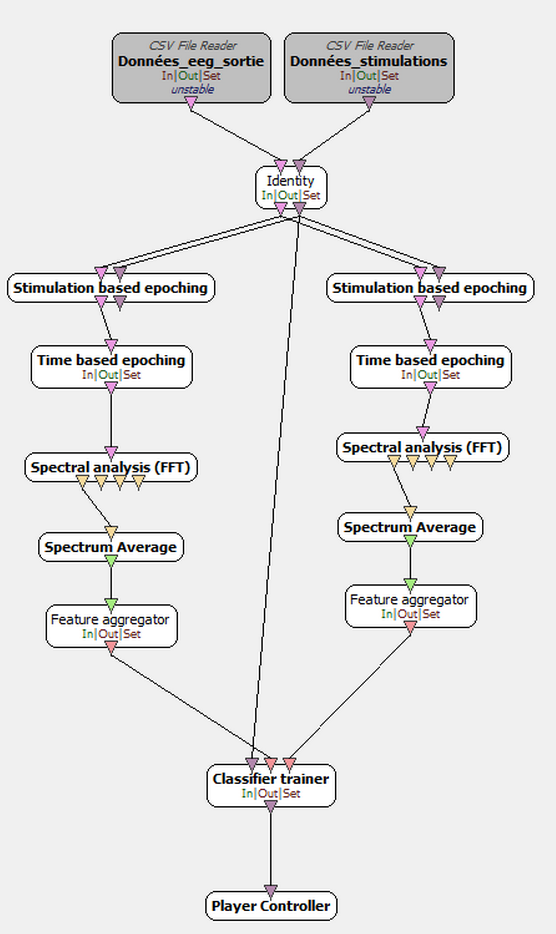
\includegraphics[height=17cm]{images/scenario_2_1.png}
				\caption{Scénario d'entrainement du classificateur à partir de fichiers .csv}
				\label{classi2}
			\end{figure}
	\smallbreak
	\item \textbf{Scénario d'exécution de l'interface cerveau-ordinateur.} Il permet d'exécuter la liaison cerveau-ordinateur (Figure \ref{obs2}). Pour cela, on utilise le fichier CSV issu du premier scénario (scénario d'acquisition) filtré spatialement avec Matlab. Le principe et la configuration du reste des blocs sont les mêmes que ceux détaillés dans la partie \ref{Subsection : 6.Scénario 4}
				\begin{figure}[h]
					\centering\includegraphics[height=14cm]{images/scenario_2_2.png}
					\caption{Scénario d'observation à partir de fichiers .csv issus de Matlab}
					\label{obs2}
				\end{figure}
	\smallbreak
\end{itemize}

\subsection{Fonctions Matlab et corrections}

Plusieurs fonctions Matlab ont été écrites par nos soins et sont fournies au professeur et aux élèves pour ce travail pratique :

\begin{itemize}
	\item \textbf{Une fonction de lecture pour les fichiers CSV}. Permet de lire les données EEG contenues dans un fichier de type .csv. Disponible en annexe.
	\item \textbf{Une fonction d'écriture pour les fichiers CSV}. Permet d'écrire dans un fichier .csv. Disponible en annexe.
	\item \textbf{Un sujet pour réaliser un filtrage ICA}. Contient la boucle de traitement à effectuer. La fonction permettant de faire un filtrage ICA reste à coder par les étudiants.
	\item \textbf{La correction pour réaliser un filtrage ICA}. Disponible en annexe.
	\item \textbf{Un sujet pour réaliser un filtrage PCA}. Contient la boucle de traitement à effectuer. La fonction permettant de faire un filtrage PCA reste à coder par les étudiants.
	\item \textbf{La correction pour réaliser un filtrage PCA}. Disponible en annexe.
\end{itemize}


\subsection{Préparation du travail pratique par le professeur}

Le TP reposant uniquement sur le scénario d'exécution de l'interface cerveau-ordinateur,  on propose deux approches pour la préparation du cours de neurosciences.

\subsubsection{Approche 1}

Dans cette approche, le professeur réalise en amont du TP l'acquisition des données pour l'entrainement du classificateur, l'acquisition des données pour l'exécution de l'interface cerveau-ordinateur et l'entrainement du classificateur.

\begin{enumerate}
	\item La première étape consiste à récupérer des données à partir du casque EEG et les données de stimulation. Pour cela, on utilisera le scénario d'acquisition. L'exécution du scénario génère alors deux fichiers CSV : 1 fichier "données\_entrée.csv" contenant les données EEG, 1 fichier "données\_stimulations.csv" l'autre les données de stimulation. Vérifiez dans le bloc "Graz Visualisation" que la case "Show instructions" est bien cochée.  
	\smallbreak 
	\item Le professeur est ensuite invité à exécuter le code Matlab "cours\_signal\_pca.m" ou "cours\_signal\_ica.m" afin de réaliser un filtrage spatial des données EEG. Veuillez pour cela à placer le fichier "données\_entrée.csv" généré dans l'étape précédente dans le même répertoire de travail que le code Matlab. Un fichier CSV "données\_EEG\_sortie.csv" contenant les signaux EEG filtrés est alors généré.
	\smallbreak
	\item On doit à présent entrainer le classificateur LDA. Pour cela, on utilise le scénario "entrainement du classificateur". On demande de fournir en entrée du scénario le fichier "données\_EEG\_sortie.csv" généré précédemment ainsi que le fichier "données\_stimulations.csv" généré lors de l'exécution du scénario "acquisition". L'exécution du scénario génère un fichier de configuration en sortie "Classifier.cfg".
	\smallbreak
	\item Enfin, on demande d'exécuter de nouveau le scénario d'acquisition afin d'obtenir des données EEG différentes de celles utilisées pour l'entrainement du classificateur afin d'exécuter l'interface cerveau-ordinateur. On veillera cette fois-ci à décocher la case "Show instructions" dans le bloc "Graz Visualisation" afin de ne pas être influencé par la présence des stimulations lors de l'acquisition des données. L'utilisateur est alors invité à penser à sa main gauche ou sa main droite chaque fois que le repère blanc apparait dans la fenêtre de visualisation (Celui-ci n'apparait qu'au bout de 30 secondes).
	\smallbreak
	\item Le professeur fournira à ses élèves le fichier de configuration du classificateur ("Classifier.cfg"), ainsi que le dernier fichier "données\_entrée.csv" généré. Cela permettra aux étudiants d'utiliser le scénario "execution de l'interface cerveau-ordinateur". 
\end{enumerate}


\subsubsection{Approche 2}
Dans cette approche, le professeur n'a pas besoin de réaliser un travail préparatoire en amont du TP (entrainement classificateur, acquisition de données EEG). Celui-ci fournit simplement à ses étudiants le fichier de configuration du classificateur et le fichier "données\_entrées.csv". Cela leur permettra d'utiliser le scénario "execution de l'interface cerveau-ordinateur".
  \chapter{Bilan du projet}
\thispagestyle{fancy}

\section {Connaissances acquises}

Ce projet captivant, de part par son originalité et son aspect pédagogique, nous a permis de mettre en application nos acquis en traitement du signal, en informatique et en neurosciences. D'un point de vue théorique, la pluridisciplinarité du sujet nous a offert l'opportunité d'acquérir de nouvelles connaissances théoriques (traitement de signaux EEG, physiologie du cerveau, etc.). Celui-ci nous a également permis d'apprendre à utiliser de nouveaux outils, comme un casque électroencéphalographique (EPOC d'Emotiv) ou encore le logiciel OpenViBE, permettant de réaliser des interfaces cerveau-ordinateur. Enfin, c'est véritablement au niveau de la méthodologie de recherche, de la gestion de projet et de l'autonomie que nous pensons avoir le plus progressé. Notons que celui-ci nous a notamment permis d'apprendre à utiliser l'outil de traitement de texte \LaTeX, afin de rédiger un rapport répondant aux normes IEEE.

\section {Problèmes rencontrés}

Notre travail devait initialement s'appuyer sur les travaux réalisés par un étudiant de la session d'automne 2014. Cependant, ses résultats ne nous semblaient pas pertinents dans le cadre de notre projet. De ce fait, nous avons décidé de reprendre le projet depuis le départ (notamment la partie portant sur le choix du matériel et du logiciel, ainsi que les traitements des signaux).

D'un point de vue théorique, les connaissances que nous avions en traitement de signaux EEG et en intelligence artificielle probabiliste étaient quasiment nulles (notamment sur l'aspect filtrage spatial et méthodes de classification). Cependant, nous pensons avoir suffisamment renforcé nos connaissances dans ces domaines.

Nous avons également rencontré certaines difficultés d'ordre pratique, notamment lors de l'intégration de notre projet dans le cours de traitement de signal avancé. Nous souhaitions en effet utiliser des outils mathématiques tel que Matlab ou Python. Cependant, leur intégration avec OpenViBE s'est avérée difficile à mettre en place (intégration de Matlab possible uniquement avec la version 32 bits, utilisation de Python trop complexe dans le cadre d'un cours). Nous sommes parvenus à trouver une solution qui consiste en l'exportation des données d'OpenViBE vers le format CSV, puis en les traitant dans Matlab. Cette manière de gérer les données EEG nous oblige cependant à ne plus réaliser la liaison cerveau-ordinateur en temps réel. Enfin, Nous avons également été confronté à quelques contraintes matérielles. La commande (et la livraison) du casque EPOC en Mars nous a obligé à implémenter l'interface cerveau-ordinateur tardivement (le travail sur l'aspect théorique du sujet a donc été privilégié dans un premier temps).

\section {Pistes d'amélioration et poursuite de nos travaux}
Par manque de temps, nous n'avons malheureusement pas pu intégrer notre expérience dans le cadre du cours d'intelligence artificielle, donné à la session d'automne. Il aurait également été intéressant d'utiliser certains outils de neurosciences computationnelles dans le cadre de notre projet, notamment pour les éléments de traitement du signal comme les filtres spatiaux ou les méthodes de classification (utilisation de réseaux neuronaux avec apprentissage).


  \chapter* {Conclusion}
\addcontentsline{toc}{chapter}{Conclusion} % Ajout dans la table des matieres
\thispagestyle{fancy}



Nous avons eu la chance de réaliser notre projet de recherche et développement (GIN956) au sein du laboratoire de recherche en neurosciences NECOTIS, sous la tutelle de Jean Rouat. Cette opportunité nous a permis de bénéficier d'une première expérience dans le monde des neurosciences, et plus particulièrement dans la conception d'une interface cerveau-ordinateur. À cette occasion, nous avons pu acquérir de nouvelles connaissances théoriques (traitement de signaux EEG, physiologie du cerveau, etc.), pratiques (utilisation d'un casque EEG, utilisation d'un logiciel de création de liaisons cerveau-ordinateur) et méthodologiques (gestion de projet, autonomie, apprentissage à l'utilisation de \LaTeX, etc.)

Dans un premier temps, nous avons étudié les différents aspects physiologiques du cerveau qui nous seraient utiles dans la réalisation de l'interface cerveau-ordinateur (organisation corticale, différents rythmes du cerveau, etc.). 

Nous avons ensuite réalisé une étude comparative des différents systèmes EEG proposés sur le marché (casques EEG, électrodes, etc). Celle-ci nous a permis d'arrêter notre choix sur le casque EPOC de la société Emotiv. Nous avons également étudié les différents logiciels libres de droit disponibles, permettant de réaliser une liaison cerveau-ordinateur. OpenViBE se trouve être l'outil informatique le plus adapté pour la réalisation de la BCI dans le cadre de notre projet. 

Dans un troisième temps, nous avons étudié différentes techniques de traitement de signaux EEG, comme les méthodes de filtrage temporel, les filtrages spatiaux ou encore les différentes techniques de classification de caractéristiques. 

Nous présentons par la suite le fonctionnement du logiciel OpenViBE et du casque EPOC, ainsi que l'ensemble des outils s'y rattachant. 

A partir de l'ensemble des études réalisées précédemment, on réalise une expérience interactive. Celle-ci s'appuie sur une chaîne de traitement et d'analyse des signaux EEG composée d'un filtrage temporel passe-bande de type Butterworth, un filtrage spatial de type CSP et une classification des caractéristiques des signaux de types LDA.

Enfin, on intégre les différents éléments de notre projet dans le cours de neurosciences computationnelles et de traitement du signal avancé, en s'appuyant sur des travaux pratiques (réalisation d'un filtrage spatial de type PCA/ICA) réalisés sous l'environnement Matlab.

  \bibliography{mybib}
  \bibliographystyle{unsrt}
  \part*{Annexes}
\addcontentsline{toc}{chapter}{Annexes} % Ajout dans la table des matieres




\subsection* {Tableau comparatif des différents casques EEG proposés sur le marché}

\begin{figure}[h]
	\centering\includegraphics[width=17cm, angle=0]{images/ComparaisonCasques.jpg}
\end{figure}




\newpage
\subsection* {Tableau comparatif des différents amplificateurs proposés sur le marché}

\begin{figure}[h]
	\centering\includegraphics[width=17cm, angle=0]{images/ComparaisonAmpli.jpg}
\end{figure}



\newpage
\subsection* {Carte heuristique}

\begin{figure}[h]
	\centering\includegraphics[width=19cm,angle=90,]{images/CarteHeuristiqueSignalProcessing.png}
\end{figure}
\newpage
\subsubsection{Sujet filtrage ICA}

\begin{verbatim}
%##########################################################################
%#####     SUJET DE TP DE COURS DE TRAITEMENT DE SIGNAL AVANCE    #########
%#######################   ICA     ########################################
%### Florian Lepont, Romain Richard######### Avril 2015####################

close all
clear all

% LECTURE DES DONNEES A PARTIR DU FICHIER CSV
donnees_eeg = lecture_csv('données_entrée.csv')

% ANALYSE EN COMPOSANTES INDEPENDANTES
sources = ica(donnees_eeg) % on récupère les données du fichier

% AFFICHAGE DES DONNNEES
subplot(2,2,1) 
plot(donnees_eeg')
xlabel('temps (s)')
ylabel('amplitude (mV)')

subplot(2,2,2)
plot(sources')
xlabel('temps (s)')
ylabel('amplitude (mV)')

subplot(2,2,3)
hist(donnees_eeg')
xlabel('amplitude (mV)')
ylabel('nombres de données')

subplot(2,2,4)
xlabel('temps (s)')
ylabel('amplitude du signal (mV)')

hist(sources')
xlabel('amplitude (mV)')
ylabel('nombres de données')

% CREATION DU FICHIER DE SORTIE
ecriture_csv( 'données_entrée.csv', 'données_EEG_sortie.csv', sources)
\end{verbatim}



\newpage
\subsubsection{Correction filtrage ICA}

\begin{verbatim}
%##########################################################################
%#####     CORRECTION FONCTION COURS TRAITEMENT SIGNAL AVANCE #############
%#######################   ICA     ########################################
%### Florian Lepont, Romain Richard######### Avril 2015####################

% Bibliographie : "A Tutorial on Independant Component Analysis" de Jonathon Shlens

function sources = ica(donnees)
% Analyse en composantes indépendantes.
% ENTREE : données à traiter
% SORTIE : Matrice de transformation linéaire, signaux sources calculés

[M,N] = size(donnees);

%  Translation de la moyenne des données vers 0.
mn = mean(donnees,2);
donnees = donnees - repmat(mn,1,N);

% Calcul de la matrice de covariance
covariance = 1 / (N-1) * (donnees * donnees');

% Calcul des valeurs propres et des vecteurs propres de la matrice de
% covariance.
[E,D] = eig(covariance);

%Calcul des données décoréllées et normalisation.
X = sqrtm(pinv(D))*E'*donnees;

%Calcul de la décomposition en valeurs singulières. (calcul de la
%transformation linéraire - rotation - V).
[V,s,u] = svd((repmat(sum(X.*X,1),M,1).*X)*X');

%Calcul de la transformation linéaire W
W = V * sqrtm(pinv(D)) * E';

%Calcul des signaux sources
sources = W * donnees;
\end{verbatim}


\newpage
\subsubsection{Sujet filtrage PCA}

\begin{verbatim}
%##########################################################################
%#######   SUJET DE TP DE COURS DE TRAITEMENT DE SIGNAL AVANCE    #########
%#########################   PCA  #########################################
%### Florian Lepont, Romain Richard######### Avril 2015####################

close all
clear all

% LECTURE DES DONNEES A PARTIR DU FICHIER CSV
donnees_eeg = lecture_csv('données_entrée.csv')

% ANALYSE EN COMPOSANTES PRINCIPALES
% On récupère les données du fichier
[signaux_pca,composantes_principales,valeurs_propres] = pca(donnees_eeg) 

% AFFICHAGE DES DONNNEES
subplot(2,2,1) 
plot(donnees_eeg')
xlabel('temps (s)')
ylabel('amplitude (mV)')

subplot(2,2,2)
plot(signaux_pca')
xlabel('temps (s)')
ylabel('amplitude (mV)')

subplot(2,2,3)
hist(donnees_eeg')
xlabel('amplitude (mV)')
ylabel('nombres de données')

subplot(2,2,4)
xlabel('temps (s)')
ylabel('amplitude du signal (mV)')

hist(signaux_pca')
xlabel('amplitude (mV)')
ylabel('nombres de données')

% CREATION DU FICHIER DE SORTIE
ecriture_csv( 'données_entrée.csv', 'données_EEG_sortie.csv', signaux_pca)
\end{verbatim}


\newpage
\subsubsection{Correction filtrage PCA}

\begin{verbatim}
%##########################################################################
%#####     CORRECTION FONCTION COURS TRAITEMENT SIGNAL AVANCE #############
%#######################   PCA     ########################################
%### Florian Lepont, Romain Richard######### Avril 2015####################

% Bibliographie : "A Tutorial on Principal Component Analysis" de Jonathon Shlens

function [signaux,composantes_principales,valeurs_propres] = pca(donnees)
% Analyse en composantes principales.
% ENTREE : données à traiter
% SORTIE : Signaux décorrélés, vecteur des composantes principales,
% vecteurs_propres

[M,N] = size(donnees);

%  Translation de la moyenne des données vers 0.
mn = mean(donnees,2);
donnees = donnees - repmat(mn,1,N);

% Calcul de la matrice de covariance
covariance = 1 / (N-1) * (donnees * donnees');

% Calcul des valeurs propres et des vecteurs propres de la matrice de
% covariance. Les vecteurs propres en sortie correspondent aux
% composantes principales.
[composantes_principales,valeurs_propres] = eig(covariance);

% Extraction des valeurs propres de la matrice vers un vecteur
valeurs_propres = diag(valeurs_propres);

% Trie des valeurs propres par ordre décroissant
[junk, indices] = sort(-1*valeurs_propres);
valeurs_propres = valeurs_propres(indices);
composantes_principales = composantes_principales(:,indices);

% On réalise la transformation linéaire des données d'entrée
signaux = composantes_principales'* donnees;
\end{verbatim}




\newpage
\subsection*{Lecture CSV}

\begin{verbatim}
%##########################################################################
%#####     FONCTION LECTURE D UNE FICHIER CSV    ##########################
%#######################   CSV     ########################################
%### Florian Lepont, Romain Richard######### Avril 2015####################

function [donnees_eeg] = lecture_csv( fichier_entree )
% Fonction lecture vers un fichier csv. La fonction permet de lire
% les données EEG contenues dans le ficher csv 'fichier_entree'. 

% EXTRACTION DES DONNEES EEG 
% Extraction des données EEG à partir du fichier CSV
% Suppression des infos temps et frequence d'échantillonnage afin de ne conserver 
% que les données des signaux
donnees_eeg(:,1) = [] 			
donnees_eeg(:,end) = []     
% Calcul de la transposée                                                
donnees_eeg = donnees_eeg'			

end
\end{verbatim}




\newpage
\subsection*{Écriture CSV}

\begin{verbatim}
%##########################################################################
%#####     FONCTION ECRITURE D UNE FICHIER CSV   ##########################
%#######################   CSV     ########################################
%### Florian Lepont, Romain Richard######### Avril 2015####################

function [] = ecriture_csv( fichier_entree, fichier_sortie, donnees)
% Fonction ecriture vers un fichier csv. La fonction permet d'ecrire
% vers le ficher csv 'fichier_sortie'. Pour cela, il récupère les 
% informations temps, fréq_echantill, colonnes et lignes à partir du
% fichier csv 'fichier_entree', généré par OpenViBE. 

% EXTRACTION DES DONNEES EEG ET CARACTERISTIQUES ACQUISITION
% Extraction des données EEG
donnees_eeg = csvread(fichier_entree,1,0);        
% Extraction de la taille du tableau de données                          
[lignes,colonnes] = size(donnees_eeg)        
% La première colonne du fichier csv correspond aux échantillons temporels                               
temps = donnees_eeg(:,1)           
% La valeurs de la dernière colonne du fichier csv correpond à la fréquence
% d'échantillonnage                                          
freq_echant = donnees_eeg(1,end)                                           

% EXTRACTION DU NOM DES VALEURS A PARTIR DU FICHIER D'ENTREE
% Ouverture du fichier csv 
fid = fopen(fichier_entree,'r');      
% On récupère les données du fichier                                      
C = textscan(fid, repmat('%s',1,colonnes), 'delimiter',',', 'CollectOutput',true); 
C = C{1};
% extraction de la première ligne du fichier, comprenant le nom des variables
nom_valeurs = C(1,:);                                                       
fclose(fid);

% CREATION DU FICHIER DE SORTIE
% Ouverture du nouveau fichier
fid1 = fopen(fichier_sortie,'w');                                           

% Concaténations des données temps et fréquence d'échantillonnage avec 
% les nouvelles valeurs décoréllées
donnees_csv = horzcat(temps, donnees')                                      
donnees_csv(:,end+1) = zeros;
donnees_csv(1,end) = freq_echant

headerFmt = repmat('%s,',1,colonnes-1); 
numFmt = repmat('%f,',1,colonnes-1);
% Écriture de l'en-tête du csv (nom des variables)
fprintf(fid1,[headerFmt,'%s\n'],nom_valeurs{1,:});    
% Écriture des données                      
fprintf(fid1,[numFmt,'%f\n'],donnees_csv');                                 

fclose(fid1)
end
\end{verbatim}


\newpage
\thispagestyle{fancy}

\begin{center}
\huge\textbf{GEI 723 : Travail pratique}
\bigbreak
\LARGE\textbf{Visualisation de signaux EEG et de l'activité cérébrale}
\bigbreak
\end{center}

\normalsize

On vous propose à travers ce travail pratique de vous familiariser avec les aspects théoriques et techniques d'une interface cerveau-ordinateur (BCI). Celle que nous vous demandons d'étudier a été mise au point sous le logiciel libre de droit OpenViBE.

\newpage
\section*{Interface cerveau-ordinateur}

L'expérience que l'on vous propose d'étudier s'appuie sur la méthode d'imagerie motrice, qui consiste à imaginer le mouvement de différentes parties du corps. Cela résulte en l'activation du cortex sensorimoteur qui module certains rythmes du cerveau. Ces variations peuvent être détectées par des électrodes EEG. L'interface cerveau-ordinateur en déduit les intentions de l'utilisateur à partir de ces signaux. Dans notre cas, celle-ci doit être capable de déterminer si l'utilisateur pense à un mouvement de sa main droite ou de sa main gauche.

La chaîne de traitement des signaux EEG de l'interface cerveau-ordintaeur se compose en 5 étapes (Figure	\ref{fig:interface_travail_ov_2}) : 

\begin{enumerate}
	\item \textbf{L'acquisition des données.} En temps normal, on récupère en temps réel les données directement issues d'un casque EEG (par exemple le casque EPOC). Comme vous ne possédez pas ce genre de casque, on vous fournit un fichier .ov contenant des signaux EEG pré-enregistrés d'une personne pensant aléatoirement à sa main gauche ou droite.
	\smallbreak
	\item \textbf{Filtrage temporel.} Ce filtrage permet d'extraire les rythmes du cerveau qui nous intéressent.
	\smallbreak
	\item \textbf{Filtrage spatial CSP.} Permet de réduire la quantité d'informations à traiter en réalisant une décorrélation et en pondérant certaines des sorties du casque. 
	\smallbreak
	\item \textbf{Analyse spectrale.} Réalise une analyse spectrale via une transformée de Fourier.
	\smallbreak
	\item \textbf{Classification.} Effectue une classification des caractéristiques à son entrée afin de déterminer à quelle main pensait l'utilisateur à un instant donné. 
\end{enumerate}

Le filtre spatial et le classificateur nécessitent d'être préalablement entrainés grâce à d'autres scénarios, générant alors un fichier de configuration pour ces deux blocs ("Classifier.cfg" et "csp-spatial-filter.cfg" ). On vous fournit ici directement ces fichiers de configuration.

\begin{figure}[h]
	\centering\includegraphics[height=12cm]{images/scenario_neuro_color.png}
	\caption{Traitement des signaux EEG sous OpenViBE.}
	\label{fig:interface_travail_ov_2}
\end{figure}


Voici la description des différents blocs utilisés dans ce scénario :

\subsubsection*{Traitement de signal}
\begin{itemize}
	\smallbreak
	\item \textbf{Temporal Filter}. Réalise le filtrage temporel d'un signal. Il est possible de choisir la méthode de filtrage (passe-bas, passe-bande ou passe-haut), le type (Butterworth, Chebychev) et l'ordre de filtre.
	\smallbreak
	\item \textbf{Spatial Filter}. Permet de réaliser du filtrage spatiale statique (filtrage bipolaire, Laplacien, etc.)
	\smallbreak
	\item \textbf{CSP Spatial Filter Trainer.} Permet de réaliser un filtrage spatial via l'algorithme CSP (voir Partie 4).
	\smallbreak
	\item  \textbf{Time Based Epoching.} Permet de découper un signal en plusieurs morceaux ayant une durée et un intervalle spécifié.
	\smallbreak
	\item \textbf{Spectral Analysis (FFT).} Réalise l'analyse spectrale de signaux en utilisant la FFT (Fast Fourier Transform).
	\smallbreak
	\item \textbf{Spectrum Average.} Calcule la moyenne de toutes les puissances de bandes de fréquences pour un spectre donné.
\end{itemize}

\subsubsection*{Classification}
\begin{itemize}
	\smallbreak
	\item \textbf{Classifier Processor.} Permet de réaliser la classification de vecteurs  caractéristiques entrants en utilisant un classificateur entrainé précédemment.
	
\end{itemize}

\subsubsection*{Lecture et écriture de fichiers}
\begin{itemize}
	\smallbreak
	\item \textbf{Generic Stream Reader.} Permet de lire un fichier enregistré grâce à un bloc Generic File Writer.
	\smallbreak
\end{itemize}

\subsubsection*{Visualisation}
\begin{itemize}
	\smallbreak
	\item\textbf{Signal Display.} Permet d'afficher un signal en temps réel.
	\smallbreak
	\item\textbf{Power Spectrum Display.} Permet d'afficher l'amplitude d'un signal dans un ensemble de bandes de fréquences.
	\smallbreak
	\item \textbf{2D Topographic Map.} Permet d'afficher la topographie de l'activité cérébrale en 2 dimensions.
	\smallbreak
	\item \textbf{3D Topographic Map.} Permet d'afficher la topographie de l'activité cérébrale en 3 dimensions.
	\smallbreak
	\item\textbf{Graz Visualisation.} Permet d'afficher la consigne et le résultat en temps réel de la première expérience que nous avons réalisé.
\end{itemize}

\subsubsection{Autres}
\begin{itemize}
	\smallbreak
	\item \textbf{Feature aggregator.} Permet de rassembler les différentes entrées du bloc vers un vecteur caractéristique.
	\smallbreak
	\item\textbf{Identity }. Duplique l'entrée de ce bloc vers sa sortie.
\end{itemize}


\newpage
\section*{OpenViBE}

\subsection*{Présentation du logiciel}

OpenViBE est une plateforme logicielle dédiée à la conception et à l'utilisation des interfaces cerveau-ordinateur en temps réel. Celle-ci est conçue par l'Institut National de Recherche en Informatique et en Automatique (INRIA) de Rennes (France). Le logiciel gère à la fois l'acquisition, le traitement et l'analyse des signaux.

Le logiciel fonctionne sous la forme de scénarios, correspondant à un ensemble de blocs fonctionnels. La suite OpenViBE est composée de deux logiciels : 
\begin{itemize}
	\item \textbf{OpenViBE designer}. Il s'agit d'un éditeur de scénario permettant de  créer et modifier des schémas blocs grâce à une interface graphique. Il suffit alors de placer les différents blocs désirés, de les configurer (en cliquant dessus) et de les relier pour former une chaine de traitement (procédure).
	\smallbreak
	\item \textbf{OpenViBE acquisition server.} Permet d'acquérir des données EEG brutes à partir de dispositifs EEG. Il est par exemple possible de connecter différents types de casques, dont le casque EPOC.
	\smallbreak
\end{itemize}

\subsection*{Téléchargement et installation d'OpenViBE}

Le logiciel fonctionne sous les systèmes d'exploitations Windows (Windows XP ou ultérieur, la stabilité du logiciel sous Windows 8 n'ayant pas été vérifiée par l'éditeur) et Linux (Ubuntu, Fedora). La liste détaillée des architectures compatibles avec OpenViBE est disponible à l'adresse suivante : http://openvibe.inria.fr/supported-architectures/.
Il est possible de télécharger l'installeur OpenViBE à l'adresse suivante : http://openvibe.inria.fr/downloads/. Une fois celui-ci téléchargé, il suffit de l'ouvrir et de suivre les indications affichées à l'écran.

\subsection*{Présentation de l'interface utilisateur d'OpenViBE Designer}

\subsubsection*{Description de l'interface de contrôle de la simulation}

La partie supérieure permet de contrôler la simulation, i.e. le déroulement du scénario. Ainsi, il est possible de lancer un scénario en appuyant sur le bouton "lecture", de le stopper en appuyant sur le bouton "stop" et d'en accélérer le déroulement en appuyant sur le bouton "avance rapide". Il est également possible de lancer plusieurs scénarios en même temps (Figure : \ref{fig:interface_simu_ov_1}). 

\begin{figure}[h]
	\centering\includegraphics[height=2cm]{images/interface_simu_ov.png}
	\caption{Interface de contrôle de la simulation sous OpenViBE.}
	\label{fig:interface_simu_ov_1}
\end{figure}

\subsubsection*{Description de l'interface du répertoire des blocs fonctionnels}

La partie située à droite de l'interface graphique du designer permet de rechercher des blocs fonctionnels afin de construire un scénario. Ceux-ci sont triés en différentes catégories. un simple glisser-déposer permet de placer un bloc dans l'espace de travail (Figure : \ref{fig:interface_bloc_ov_1}).

\begin{figure}[h]
	\centering\includegraphics[height=7cm]{images/interface_bloc_ov.png}
	\caption{Interface du répertoire des blocs OpenViBE.}
	\label{fig:interface_bloc_ov_1}
\end{figure}

\subsubsection*{Description de l'espace de travail}

La partie centrale de l'interface graphique correspond à l'espace de travail d'OpenViBE. C'est ici où l'on construit les différents scénarios de l'interface cerveau-ordinateur, via des blocs fonctionnels. Chaque bloc peut être relié à un autre. On peut seulement connecter une entrée à une sortie du même type (e.g. une entrée de type "signal" vers une sortie de type "signal") (Figure : \ref{fig:interface_travail_ov_1}).

\begin{figure}[h]
	\centering\includegraphics[height=8cm]{images/interface_travail_ov.png}
	\caption{Espace de travail d'OpenViBE.}
	\label{fig:interface_travail_ov_1}
\end{figure}


\newpage
\section*{Manipulation}

\begin{enumerate}
	\smallbreak
	\item Commencez par télécharger et installer OpenViBE.
	\smallbreak
	\item Une fois OpenViBE installé, ouvrez le fichier "online-neuroscience.xml". Il s'agit du scénario comprenant la chaîne de traitement des signaux EEG. 
	\smallbreak
	\item Double-cliquez sur le bloc "Generic Stream Reader" et indiquez le chemin vers le fichier "motor-imagery-csp.ov" qui vous a été fourni. 
	\smallbreak
	\item Double-cliquez sur le bloc "csp-spatial-filter.cfg" et indiquez le chemin vers le fichier csp-spatial-filter.cfg" qui vous a été fourni. 
	\smallbreak
	\item Double-cliquez sur le bloc "Classifier Processor" et indiquez le chemin vers le fichier "classifier.cfg" qui vous a été fourni.
	\smallbreak
	\item Double-cliquez sur le bloc "Graz motor imagery bci simulator" et indiquez le chemin vers le fichier "motor-imagery-bci-graz-stimulator.lua" qui vous a été fourni.
	\smallbreak
	\item Démarrez l'interface cerveau-ordinateur en cliquant sur le bouton "lecture".
\end{enumerate}

\section*{Questions}

\begin{enumerate}
	\smallbreak
	\item Une fois le scénario lancé, aucune activité cérébrale n'apparait dans la fenêtre de visualisation. Le filtre temporel passe-bande a été configuré pour ne laisser passer aucun signal (fréquences de coupures 0Hz, 0Hz). Sachant que l'on souhaite dans le cadre de notre application extraire uniquement certains rythmes du cerveau, comment devez-vous configurer le filtre temporel ? Modifiez la configuration du filtre en double-cliquant dessus. 
	\smallbreak
	\item Quel est le nom des rythmes que l'on souhaite conserver ? 
	\smallbreak
	\item Observez les différentes étapes de traitement des signaux EEG. 
	\smallbreak
	\item L'analyse spectrale des signaux est effectuée avec une FFT. Est-ce la solution la plus optimale ? Pourquoi ? 
	\smallbreak
	\item Proposez une autre solution d'analyse spectrale. 
\end{enumerate}

\newpage
\thispagestyle{fancy}

\begin{center}
	\huge\textbf{GEI 752 : Travail pratique}
	\bigbreak
	\LARGE\textbf{Traitement de signaux EEG et applications dans une interface cerveau-ordinateur}
	\bigbreak
\end{center}

\normalsize

On vous propose à travers ce travail pratique de vous familiariser avec les aspects théoriques et techniques d'une interface cerveau-ordinateur et d'utiliser vos connaissances en traitement du signal afin de participer à la conception de la chaine de traitement des données électroencéphalographiques (EEG).

\newpage
\section*{Interface cerveau-ordinateur}

Une interface Cerveau-Ordinateur ou BCI (Brain Computer Interface) est une interface permettant de réaliser une communication allant du cerveau vers un système numérique (ordinateur par exemple). Pour cela, on s'appuie sur une étude de l'activité neuronale du cerveau grâce à un système électroencéphalographique (EEG) utilisant des électrodes. Celles-ci sont placées à la surface du crâne afin de capter son activité électrique. Un traitement et une analyse des signaux électriques saisis sont réalisés afin de les traduire en informations exploitables par les systèmes numériques. L'expérience que l'on vous propose d'étudier ici s'appuie sur la méthode d'imagerie motrice, qui consiste à imaginer le mouvement de différentes parties du corps. Cela résulte en l'activation du cortex sensorimoteur qui module certains rythmes du cerveau. Ces variations peuvent être détectées par des électrodes EEG. L'interface cerveau-ordinateur en déduit les intentions de l'utilisateur à partir de ces signaux. Dans notre cas, celle-ci doit être capable de déterminer si l'utilisateur pense à un mouvement de sa main droite ou de sa main gauche.

La chaîne de traitement des signaux EEG de l'interface cerveau-ordinateur se compose de 5 étapes (Figure	\ref{fig:interface_travail_ov_5}) : 

\begin{enumerate}
	\item \textbf{L'acquisition des données.} En temps normal, on récupère les données directement issues d'un casque EEG (par exemple le casque EPOC de la société Emotiv). Comme vous ne possédez pas ce genre de casque, on vous fournit un fichier .csv contenant des signaux EEG pré-enregistrés d'une personne pensant aléatoirement à sa main gauche ou droite.
	\smallbreak
	\item \textbf{Filtrage temporel.} Ce filtrage permet d'extraire les rythmes du cerveau qui nous intéressent.
	\smallbreak
	\item \textbf{Filtrage spatial.} On souhait utiliser un filtrage spatial afin d'optimiser nos données. Il vous sera demandé ultérieurement d'implémenter ce filtre sous Matlab. 
	\item \textbf{Filtrage spatial CSP.} Permet de réduire la quantité d'informations à traiter en réalisant une décorrélation et en pondérant certaines des sorties du casque. 
	\smallbreak
	\item \textbf{Analyse spectrale.} Réalise une analyse spectrale via une transformée de Fourier.
	\smallbreak
	\item \textbf{Classification.} Effectue une classification des caractéristiques présentes à son entrée afin de déterminer à quelle main pensait l'utilisateur à un instant donné. 
\end{enumerate}

Le classificateur nécessite d'être préalablement entrainé grâce à d'autres scénarios, qui génèrent alors son fichier de configuration. On vous fournit directement le fichier de configuration ("classifier.cfg"). Veuillez également noter que vous ne possédez pas le scénario d'acquisition permettant de récupérer les données EEG. On vous fournit donc également les données filtrées temporellement dans le fichier ("données\_entrée.csv").

\begin{figure}[h]
	\centering\includegraphics[height=10cm]{images/sujet_signal_color.png}
	\caption{Traitement des signaux EEG sous OpenViBE.}
	\label{fig:interface_travail_ov_5}
\end{figure}

\newpage
\section*{OpenViBE}

\subsection*{Présentation du logiciel}

OpenViBE est une plateforme logicielle dédiée à la conception et à l'utilisation d'interfaces cerveau-ordinateur en temps réel. Celle-ci est éditée par l'Institut National de Recherche en Informatique et en Automatique (INRIA) de Rennes (France). Le logiciel gère à la fois l'acquisition, le traitement et l'analyse des signaux.

Le logiciel fonctionne sous la forme de scénarios, correspondant à un ensemble de blocs fonctionnels. La suite OpenViBE est composée de deux logiciels : 
\begin{itemize}
	\item \textbf{OpenViBE designer}. Il s'agit d'un éditeur de scénario permettant de  créer et modifier les schémas blocs grâce à une interface graphique. Il suffit alors de placer les différents blocs, de les configurer (en cliquant dessus), et de les relier pour former une chaine de traitement.
	\smallbreak
	\item \textbf{OpenViBE acquisition server.} Permet d'acquérir des données EEG brutes à partir de dispositifs EEG. Il est par exemple possible de connecter différents types de casques, dont le casque EPOC.
	\smallbreak
\end{itemize}

\subsection*{Téléchargement et installation d'OpenViBE}

Le logiciel fonctionne sous les systèmes d'exploitations Windows (Windows XP ou ultérieur, la stabilité du logiciel sous Windows 8 n'ayant pas été vérifiée par l'éditeur) et Linux (Ubuntu, Fedora). La liste détaillée des architectures compatibles avec OpenViBE est disponible à l'adresse suivante : http://openvibe.inria.fr/supported-architectures/.
Il est possible de télécharger l'installeur OpenViBE à l'adresse suivante : http://openvibe.inria.fr/downloads/. Une fois celui-ci téléchargé, il suffit de l'ouvrir et de suivre les indications affichées à l'écran.

\subsection*{Présentation de l'interface utilisateur d'OpenViBE Designer}

\subsubsection*{Description de l'interface de contrôle de la simulation}

La partie supérieure de l'interface graphique permet de contrôler la simulation, i.e. le déroulement du scénario. Ainsi, il est possible de lancer un scénario en appuyant sur le bouton "lecture", de le stopper en appuyant sur le bouton "stop" et d'en accélérer le déroulement en appuyant sur le bouton "avance rapide". Il est également possible de lancer plusieurs scénarios en même temps (Figure : \ref{fig:interface_simu_ov_2}). 

\begin{figure}[h]
	\centering\includegraphics[height=2cm]{images/interface_simu_ov.png}
	\caption{Interface de contrôle de la simulation sous OpenViBE.}
	\label{fig:interface_simu_ov_2}
\end{figure}

\subsubsection*{Description de l'interface du répertoire des blocs fonctionnels}

La partie située à droite de l'interface graphique du designer permet de rechercher les blocs afin de construire un scénario. Ceux-ci sont triés en différentes catégories. un simple glisser-déposer permet de placer un bloc dans l'espace de travail (Figure : \ref{fig:interface_bloc_ov_2}).

\begin{figure}[h]
	\centering\includegraphics[height=7cm]{images/interface_bloc_ov.png}
	\caption{Interface du répertoire des blocs OpenViBE.}
	\label{fig:interface_bloc_ov_2}
\end{figure}

\subsubsection*{Description de l'espace de travail}

La partie centrale de l'interface graphique correspond à l'espace de travail d'OpenViBE. C'est ici que l'on construit les différents scénarios de l'interface cerveau-ordinateur, via des blocs fonctionnels. Chaque bloc peut être relié à un autre. On peut seulement connecter une entrée à une sortie du même type (e.g. une entrée de type "signal" vers une sortie de type "signal") (Figure : \ref{fig:interface_travail_ov_4}).

\begin{figure}[h]
	\centering\includegraphics[height=8cm]{images/interface_travail_ov.png}
	\caption{Espace de travail d'OpenViBE.}
	\label{fig:interface_travail_ov_4}
\end{figure}


\newpage

\section*{Manipulation}

\begin{enumerate}
	\smallbreak
	\item Commencez dans un premier temps par télécharger et installer OpenViBE. Celui-ci vous servira dans la question 3. 
	\smallbreak
	\item On vous demande de coder un filtre spatial PCA sous Matlab et de traiter les données EEG contenues dans le fichier "données\_entrée.csv". Le code Matlab n'étant pas directement exécutable dans OpenViBE, vous devez utiliser la fonction Matlab "lecture\_csv.m" afin d'extraire les données EEG du fichier "données\_entrée.csv", ainsi que la fonction "ecriture\_csv.m" afin d'écrire les données après filtrage spatial vers le fichier CSV "données\_EEG\_sortie.csv".
	\smallbreak
	\item Une fois le code implémenté et vos données filtrées, on exporte les signaux vers OpenViBE. Pour cela, démarrez OpenViBE. Ouvrez ensuite le fichier "online.xml".
	\smallbreak
	\item Double-cliquez sur le bloc "CSV File Reader" et indiquez le chemin vers le fichier que vous avez généré à partir de votre code Maltab. Par défaut, ce fichier s'appelle "données\_EEG\_sortie.csv". 
	\smallbreak
	\item Double-cliquez sur le bloc "Classifier Processor" et indiquez le chemin vers le fichier "classifier.cfg" qui vous a été fourni.
	\smallbreak
	\item Double-cliquez sur le bloc "Graz motor imagery bci simulator" et indiquez le chemin vers le fichier "motor-imagery-bci-graz-stimulator.lua" qui vous a été fourni.
	\smallbreak
	\item Démarrez l'interface cerveau-ordinateur en cliquant sur le bouton "lecture". Qu'observez vous dans la fenêtre de visualisation ? 
	\smallbreak 
	\item De la même manière que dans la question 2, on vous demande à présent d'implémenter un filtre spatial ICA sous Matlab. Exportez de nouveau vos données vers OpenViBE. Qu'observez vous ? 
\end{enumerate}



\newpage



%\includepdf[pages=1]{pdf/Sujet_GEI723.pdf}
\end{document}

